% !TEX program = xelatex
\documentclass{yupin-notes}
\usepackage{yp-figures}
% 本书 TikZ 图的共用样式（正文与网页的单独编译都会读入）
\tikzset{
  gv/.style    = {circle, draw, thick, fill=white, minimum size=6.2mm, inner sep=0pt, font=\small},
  gvh/.style   = {gv, fill=RainbowAmber!35},            % 高亮的顶点
  gvd/.style   = {gv, fill=black!12},                    % 已处理的顶点
  ge/.style    = {thick},
  geh/.style   = {line width=2.2pt, RainbowBlue},        % 高亮的边
  arc/.style   = {thick, -{Stealth[length=2.6mm]}},
  arch/.style  = {line width=1.8pt, RainbowBlue, -{Stealth[length=3mm]}},
  geo/.style   = {line width=2.2pt, RainbowAmber},       % 第二种高亮（两条路并列时）
  archo/.style = {line width=1.8pt, RainbowAmber, -{Stealth[length=3mm]}},
  wt/.style    = {font=\footnotesize, fill=white, inner sep=1pt},
  cell/.style  = {draw, minimum width=7.5mm, minimum height=6mm, inner sep=0pt, font=\small\ttfamily},
  cellh/.style = {cell, fill=RainbowAmber!35},
  idx/.style   = {font=\scriptsize\ttfamily, text=black!55},
  ptr/.style   = {thick, -{Stealth[length=2.2mm]}},
}

\coursetitle{图论、概率组合与组合优化}
\coursekind{例题与方法}
\coursesubtitle{图论：讲义第 1 章的例题、习题与练习}
\homeworkheader{图论，练习 #1}
\homeworkrules{练习供自学使用。每道题后面紧跟解答，网页上默认折叠，建议先自己想一想再展开。}


\begin{document}
\makecoursetitle
% 说明：本书的来源、编排与标注，讲义勘误
\frontsection{说明}

这里收的是图论课讲义中不平凡的部分：讲义没有证明或证明不完整的定理，不平凡的例题与课后题的解答，以及对其中经典方法的归纳。定义和简单的题（画图、写矩阵、直接套定义）不收。

内容按方法编排，不按讲义的章节。每一讲讲一种（或两三种相关的）方法：开头说明方法的要点，然后是例题；讲后的作业是新出的练习，用来熟悉这些方法，每题后面都有解答，网页上默认折叠。

\subsection*{标注}

出自讲义的内容，在开头用括号注明，如“（讲义定理 1.4）”“（讲义习题 1.8）”“（讲义问答题 1.3）”。没有注明的是补充的。

\subsection*{讲义勘误}

下面几道讲义习题的原文有误。每题开头的注记给出反例与猜测的原题，解答证明的是猜测的版本。

\begin{enumerate}
\item 习题 1.9（\wegref{we:longest-paths:dirac}）：“长度至少为 $\min\{2\delta,\abs G\}$ 的路或圈”对 $K_2$ 不成立；应为“长度至少为 $\min\{2\delta,\abs G-1\}$ 的路”。
\item 习题 1.12（\wegref{we:double-counting:games}）：“$n$ 个球队赛完 $n-1$ 场，必有一队至少赛过 $3$ 场”不成立（各队排成一列，相邻两队各赛一场）；应为“赛完 $n+1$ 场”。
\item 习题 1.17（\wegref{we:distance-layers:equal-distance}）：对不连通的图不成立（$K_2\cup K_1$）；应限定 $G$ 连通。
\end{enumerate}
另有一处措辞需要澄清：习题 1.8（\wegref{we:longest-paths:sqrt-k}）中“连接它们之间的路的长度至少为 $k$”应理解为存在这样一条路，而不是两点的距离至少为 $k$。

\subsection*{没有收的讲义习题}

第 1 章：习题 1、2、3、5、6、7、14、15、19、20，问答题 1.1、1.2、1--4、1--5。

\tableofcontents

\coursepart{图论}
% 讲义第 1、2 章，按方法重新编排
% !TEX root = ../graph-theory.tex
% =====================================================================
%  极端选择：最长路；删点：平均度与最小度；最大割
% =====================================================================
\lecture{极端选择与删点：最长路给出长圈与偶圈，长路与 Dirac 定理，圈外的长路，平均度与最小度，树的贪心嵌入，最大割与二部子图}
\label{lec:longest-paths}

这一讲收两种最常用的方法。第一种是取一个极端的对象，通常是一条最长路，然后说明“如果结论不成立，就能得到更长的路”。第二种是反复删掉度数小的顶点，把关于平均度（也就是边数）的条件变成关于最小度的条件；与它配套的是最大割，它把任意图变成边数至少一半的二部图。

\topic{方法：取一条最长路}

设 $P=v_0v_1\dots v_\ell$ 是 $G$ 中的一条最长路。
\begin{enumerate}
\item 端点 $v_0$ 的邻点全在 $P$ 上。否则 $v_0$ 的一个 $P$ 外的邻点 $u$ 给出更长的路 $uv_0v_1\dots v_\ell$。所以 $d(v_0)\geqslant\delta$ 个邻点都落在 $\{v_1,\dots,v_\ell\}$ 中，于是 $\ell\geqslant\delta$。
\item 若 $v_0v_j$ 是边，则 $v_0v_1\dots v_jv_0$ 是长为 $j$ 的圈。取 $j$ 为最大的这种下标，就得到长圈；比较几个邻点下标的奇偶，就得到偶圈。
\item 把两个端点的邻点下标放在一起，用鸽笼原理找一个 $i$ 使 $v_0v_{i+1}$ 与 $v_iv_\ell$ 都是边，就得到一个经过 $P$ 的全部顶点的圈 $v_0v_{i+1}v_{i+2}\dots v_\ell v_iv_{i-1}\dots v_1v_0$。若图连通而 $P$ 不含全部顶点，这个圈加上一条伸出去的边又给出更长的路。
\item 有向图中把“邻点”换成“出邻点”（或“入邻点”），论证不变。
\end{enumerate}
同一个想法的变体：取最长圈、最短圈、边数最少的反例、极大的某种子图。关键是先想清楚：如果结论不成立，能把这个对象改得更极端吗？

\begin{theorem}\label{thm:longest-paths:long-cycle}
（讲义定理 1.4）设 $G$ 是简单图，$\delta(G)\geqslant2$。则 $G$ 含有长度至少为 $\delta(G)+1$ 的圈。若 $\delta(G)\geqslant3$，则 $G$ 含有偶圈。
\end{theorem}
\begin{proof}
设 $P=v_1v_2\dots v_k$ 是最长路。$v_1$ 的邻点都在 $P$ 上，设 $j$ 是满足 $v_1v_j\in E$ 的最大下标。$v_1$ 至少有 $\delta$ 个邻点，都在 $\{v_2,\dots,v_j\}$ 中，所以 $j-1\geqslant\delta$。圈 $v_1v_2\dots v_jv_1$ 的长度是 $j\geqslant\delta+1$。

设 $\delta\geqslant3$，取 $v_1$ 的两个邻点 $v_i,v_j$，$2<i<j$。圈 $v_1v_2\dots v_iv_1$ 长为 $i$，圈 $v_1v_2\dots v_jv_1$ 长为 $j$，圈 $v_1v_iv_{i+1}\dots v_jv_1$ 长为 $j-i+2$。若 $i,j$ 中有偶数，前两个圈之一是偶圈；若 $i,j$ 都是奇数，$j-i+2$ 是偶数。
\end{proof}

\begin{remark}
讲义中的条件“$n\geqslant3$”是多余的：$\delta\geqslant2$ 的简单图至少有三个顶点。界 $\delta+1$ 不能改进：$K_{\delta+1}$ 的最长圈长度恰为 $\delta+1$。
\end{remark}

\begin{workedexample}\label{we:longest-paths:digraph-cycle}
（讲义问答题 1.3）设 $D$ 是简单有向图，$\delta^+(D)\geqslant1$。证明 $D$ 含有有向圈。更一般地，若 $\delta^+(D)\geqslant k\geqslant1$，则 $D$ 含有长度至少为 $k+1$ 的有向圈。
\end{workedexample}
\begin{solution}
设 $P=v_1v_2\dots v_m$ 是最长的有向路。$v_m$ 的每个出邻点都在 $P$ 上，否则可以把 $P$ 延长。$v_m$ 没有环，所以它的至少 $k$ 个出邻点都在 $\{v_1,\dots,v_{m-1}\}$ 中，其中下标最小的一个 $v_i$ 满足 $i\leqslant m-k$。于是 $v_iv_{i+1}\dots v_mv_i$ 是长度为 $m-i+1\geqslant k+1$ 的有向圈。$k=1$ 就是第一问（这里长度为 $2$ 的有向圈 $v_{m-1}v_mv_{m-1}$ 也算圈）。
\end{solution}

\begin{workedexample}\label{we:longest-paths:dirac}
（讲义习题 1.9）证明：每个连通图 $G$ 都含有一条长度至少为 $\min\{2\delta(G),\abs G-1\}$ 的路。若 $\abs G\geqslant3$ 且 $\delta(G)\geqslant\abs G/2$，则 $G$ 有 Hamilton 圈（Dirac 定理）。
\end{workedexample}
\begin{remark}[讲义原题有误]
讲义的题目是“每个连通图都包含一条长度至少为 $\min\{2\delta(G),\abs G\}$ 的路或圈”。$K_2$ 是反例：$\delta=1$，$\min\{2,2\}=2$，但 $K_2$ 只有一条长为 $1$ 的路，没有圈。原题应当是 Diestel 书中的习题，即上面的第一句。$\abs G\geqslant3$ 时讲义的说法也成立：$2\delta<\abs G$ 时由第一句得到长 $\geqslant2\delta$ 的路，$2\delta\geqslant\abs G$ 时由第二句得到长为 $\abs G$ 的圈。
\end{remark}
\begin{solution}
设 $P=v_0v_1\dots v_\ell$ 是最长路。我们证明：若 $\ell<2\delta$，则 $G$ 有一个恰好经过 $P$ 的全部顶点的圈 $C$。

$v_0$ 与 $v_\ell$ 的邻点都在 $P$ 上。令
\[
A=\{i\in\{0,\dots,\ell-1\}: v_0v_{i+1}\in E\},\qquad B=\{i\in\{0,\dots,\ell-1\}: v_iv_\ell\in E\}.
\]
$\abs A=d(v_0)\geqslant\delta$，$\abs B=d(v_\ell)\geqslant\delta$，而 $A,B\subseteq\{0,\dots,\ell-1\}$ 只有 $\ell<2\delta$ 个元素，所以存在 $i\in A\cap B$。令
\[
C=v_0v_{i+1}v_{i+2}\dots v_\ell v_iv_{i-1}\dots v_1v_0 .
\]
（$i=0$ 时 $C=v_0v_1\dots v_\ell v_0$。）$C$ 经过 $v_0,\dots,v_\ell$ 各一次。要使 $C$ 是圈还需 $\ell\geqslant2$：$\delta\geqslant1$ 时 $\ell\geqslant\delta$；若 $\ell=1$，则 $\delta=1$ 且 $\ell<2=2\delta$，这时 $G$ 连通、最长路长为 $1$，$G=K_2$，结论 $\ell\geqslant\min\{2,1\}$ 成立。下设 $\ell\geqslant2$。

现在设 $\ell<\min\{2\delta,\abs G-1\}$。由上面，$C$ 是含 $\ell+1<\abs G$ 个顶点的圈。$G$ 连通，所以有 $C$ 外的顶点 $u$ 与 $C$ 上某个顶点 $w$ 相邻。从 $u$ 出发走到 $w$，再沿 $C$ 绕一圈到 $w$ 在 $C$ 上的一个邻点为止，得到长为 $\ell+1$ 的路，与 $P$ 最长矛盾。所以 $\ell\geqslant\min\{2\delta,\abs G-1\}$。

Dirac 定理：$\delta\geqslant\abs G/2$ 时任意两个不相邻的顶点有公共邻点（$\abs{N(x)}+\abs{N(y)}\geqslant\abs G>\abs{V\setminus\{x,y\}}$），所以 $G$ 连通。$\delta\geqslant3/2$，故 $\delta\geqslant2$，$\ell\geqslant\delta\geqslant2$。最长路的长度 $\ell\leqslant\abs G-1<2\delta$，由上面得到经过 $P$ 全部顶点的圈 $C$；若 $\ell<\abs G-1$，刚才的论证给出更长的路，矛盾。所以 $\ell=\abs G-1$，$C$ 是 Hamilton 圈。
\end{solution}

\begin{workedexample}\label{we:longest-paths:sqrt-k}
（讲义习题 1.8）设图 $G$ 含有圈 $C$，并且 $G$ 中有一条长度至少为 $k$ 的路，它的两个端点在 $C$ 上。证明 $G$ 含有长度至少为 $\sqrt k$ 的圈。
\end{workedexample}
\begin{remark}
讲义写的是“$C$ 包含两个顶点，使得连接它们之间的路在 $G$ 中的长度至少为 $k$”。如果理解成这两个顶点在 $G$ 中的\emph{距离}至少为 $k$，那么 $C$ 本身的长度就至少是 $2k$，题目是平凡的。所以应当理解成“存在一条长度至少为 $k$ 的路”，这也是 Diestel 书中的原题。
\end{remark}
\begin{solution}
不妨设 $\abs C<\sqrt k$（否则 $C$ 就是所求的圈）。设 $P$ 是长度 $\geqslant k$ 的路，端点 $x\neq y$ 都在 $C$ 上。沿 $P$ 从 $x$ 走到 $y$，依次记下 $P$ 落在 $C$ 上的顶点 $x=u_0,u_1,\dots,u_r=y$。它们是 $C$ 的不同顶点，所以 $r+1\leqslant\abs C<\sqrt k$，$r<\sqrt k$。

这些点把 $P$ 分成 $r$ 段 $P_s=P[u_{s-1},u_s]$，每段的内部顶点都不在 $C$ 上。总长度至少为 $k$，所以有一段的长度 $q\geqslant k/r>k/\sqrt k=\sqrt k$。$u_{s-1}\neq u_s$ 把 $C$ 分成两条弧，取其中一条弧 $Q$，$P_s\cup Q$ 是一个圈（$P_s$ 与 $Q$ 只在两个端点相交），长度至少为 $q+1>\sqrt k$。
\end{solution}

\begin{remark}
这里用到的是另一种极端选择：在 $P$ 被 $C$ 截成的各段中取最长的一段。这样的段称为 $C$-路，它与 $C$ 的一条弧总能拼成圈。
\end{remark}

\topic{方法：删掉度数小的顶点}

关于边数的条件（$m\geqslant cn$，或者平均度 $d(G)\geqslant2c$）不能直接使用，因为可能有很多度数很小的顶点。办法是把度数不超过当前 $\varepsilon=m/n$ 的顶点一个一个删掉：删一个顶点，顶点数少 $1$，边数至多少 $\varepsilon$，所以比值 $\varepsilon$ 不减。删不动的时候，剩下的子图的最小度大于它自己的 $\varepsilon$。这样就把“平均度大”换成了“某个子图的最小度大”，然后可以用最长路、贪心嵌入等需要最小度的论证。

\begin{theorem}\label{thm:longest-paths:min-degree-subgraph}
（讲义定理 1.3）记 $\varepsilon(G)=\abs{E(G)}/\abs G$。每个至少有一条边的图 $G$ 都有子图 $H$，满足 $\delta(H)>\varepsilon(H)\geqslant\varepsilon(G)$。
\end{theorem}
\begin{proof}
令 $G_0=G$。若 $G_i$ 有顶点 $v$ 使 $d_{G_i}(v)\leqslant\varepsilon(G_i)$，令 $G_{i+1}=G_i-v$；否则停止，令 $H=G_i$。设 $G_i$ 有 $n_i$ 个顶点、$m_i$ 条边。若 $n_i\geqslant2$，
\[
\varepsilon(G_{i+1})=\frac{m_i-d_{G_i}(v)}{n_i-1}\geqslant\frac{m_i-m_i/n_i}{n_i-1}=\frac{m_i}{n_i}=\varepsilon(G_i).
\]
所以 $\varepsilon(G_i)\geqslant\varepsilon(G)>0$ 对每个出现的 $G_i$ 成立。单个顶点的图 $\varepsilon=0$，所以序列不会走到单点，上面的计算始终有 $n_i\geqslant2$。过程在有限步内停止，停止时 $H$ 中没有顶点满足 $d_H(v)\leqslant\varepsilon(H)$，即 $\delta(H)>\varepsilon(H)\geqslant\varepsilon(G)$。
\end{proof}

\begin{workedexample}\label{we:longest-paths:tree-embedding}
（讲义推论 1.3、1.4）设 $T$ 是树，$\delta(G)\geqslant\abs T-1$。证明 $G$ 含有同构于 $T$ 的子图。由此证明：若 $\abs{E(G)}\geqslant(t-2)\abs G$ 且 $\abs{E(G)}\geqslant1$，则 $G$ 含有每一棵 $t$ 个顶点的树。
\end{workedexample}
\begin{solution}
先把 $T$ 的顶点排成 $v_1,\dots,v_t$，使每个 $v_i$（$i\geqslant2$）在 $\{v_1,\dots,v_{i-1}\}$ 中恰有一个邻点（讲义推论 1.3）。这可以这样得到：从任一顶点出发，每次加入一个与已选顶点相邻的新顶点（$T$ 连通，所以总能加入）；新顶点若在已选部分有两个邻点，则这两条边与已选部分（连通）中连接这两个邻点的路构成圈，矛盾。

现在贪心地嵌入。把 $v_1$ 映到 $G$ 的任一顶点。设 $v_1,\dots,v_{i-1}$ 已经映到不同的顶点 $\varphi(v_1),\dots,\varphi(v_{i-1})$，且保持邻接。$v_i$ 的唯一前邻点 $v_p$ 的像 $\varphi(v_p)$ 至少有 $\delta(G)\geqslant t-1$ 个邻点，其中至多 $i-2\leqslant t-2$ 个已被使用（除 $\varphi(v_p)$ 外的已用顶点），所以有一个未用的邻点，把 $v_i$ 映到它。$i=t$ 时得到 $T$ 的一个拷贝。

第二问：$\varepsilon(G)\geqslant t-2$。由定理~\ref{thm:longest-paths:min-degree-subgraph}，有子图 $H$ 满足 $\delta(H)>\varepsilon(H)\geqslant t-2$，即 $\delta(H)\geqslant t-1$。由第一问，$H$ 含有每一棵 $t$ 个顶点的树。
\end{solution}

\begin{remark}
Erdős--Sós 猜想说 $\abs{E(G)}>\frac{t-2}2\abs G$ 就足够，比上面的界小一半。$K_{t-1}$ 的不交并说明这个界如果成立就是最好的。
\end{remark}

\topic{方法：最大割}

把 $V(G)$ 分成两部分 $(A,B)$，使跨越两部分的边数 $e(A,B)$ 最大。若某个顶点 $v\in A$ 在 $A$ 中的邻点多于在 $B$ 中的邻点，把 $v$ 移到 $B$，$e(A,B)$ 严格增大，矛盾。所以：

\begin{lemma}\label{lem:longest-paths:max-cut}
每个图 $G$ 的顶点集都有划分 $(A,B)$，使每个顶点在自己那一部分中的邻点数不超过它在另一部分中的邻点数。于是二部子图 $G[A,B]$（只保留跨越的边）满足 $d_{G[A,B]}(v)\geqslant d_G(v)/2$ 对一切 $v$ 成立，边数至少为 $\abs{E(G)}/2$。
\end{lemma}
\begin{proof}
取使 $e(A,B)$ 最大的划分，用上面的论证。第二句：每个顶点至少一半的边跨越两部分，对 $v$ 求和得边数的结论。
\end{proof}

这是“局部调整”的最简单的例子：取一个使某个量最大（或最小）的对象，然后说明任何一个顶点的移动都不能改进它。第 2 章的 Lovász 划分定理用的是同样的论证，只是把 $e(A,B)$ 换成了加权的量。

\begin{workedexample}\label{we:longest-paths:bipartite-subgraph}
（讲义习题 1.18）求函数 $f:\N\to\N$，使对每个 $k\in\N$，平均度至少为 $f(k)$ 的图都有最小度至少为 $k$ 的二部子图。
\end{workedexample}
\begin{solution}
取 $f(k)=4k$。设 $d(G)\geqslant4k$，则 $G$ 至少有一条边。由引理~\ref{lem:longest-paths:max-cut}，$G$ 有生成二部子图 $B$，边数至少为 $\abs{E(G)}/2$，所以
\[
\varepsilon(B)=\frac{\abs{E(B)}}{\abs G}\geqslant\frac{\abs{E(G)}}{2\abs G}=\frac{d(G)}4\geqslant k .
\]
由定理~\ref{thm:longest-paths:min-degree-subgraph}，$B$ 有子图 $H$ 满足 $\delta(H)>\varepsilon(H)\geqslant k$。二部图的子图仍是二部图，所以 $H$ 就是所求的子图。

两步也可以交换：先由定理~\ref{thm:longest-paths:min-degree-subgraph} 取子图 $H_0$，$\delta(H_0)>d(G)/2\geqslant2k$，再对 $H_0$ 用引理~\ref{lem:longest-paths:max-cut}，得到的二部子图中每个顶点保留至少一半的度数，最小度大于 $k$。常数还可以略为改进：$\delta(H)>\varepsilon(H)\geqslant d(G)/4$，所以 $k\geqslant2$ 时 $f(k)=4k-4$ 就够了。
\end{solution}

\topic{小结}

\begin{itemize}
\item 最长路的端点把全部邻点“关”在路上。由此得到长圈（定理~\ref{thm:longest-paths:long-cycle}）、有向圈、Dirac 定理（\wegref{we:longest-paths:dirac}）。
\item 删掉度数不超过 $\varepsilon$ 的顶点不降低 $\varepsilon$，所以平均度大的图有最小度大的子图（定理~\ref{thm:longest-paths:min-degree-subgraph}），再与最小度的论证（贪心嵌入、最长路）配合。
\item 最大割是局部调整的原型：最优的划分中，没有顶点愿意换边。
\end{itemize}

\homework{最长路、删点与最大割的练习}[最长路、删点与最大割]

\exercisepart{练习}

\begin{exercises}{A}{最长路与极端选择}
\item\label{ex:longest-paths:A1} 证明：若 $\delta(G)\geqslant3$，则 $G$ 含有一个带弦的圈（弦是连接圈上两个不相邻顶点的边）。
\begin{solution}
取最长路 $P=v_1\dots v_k$。$v_1$ 的至少三个邻点都在 $P$ 上，设为 $v_2,v_i,v_j$，$2<i<j$。圈 $C=v_1v_2\dots v_jv_1$ 上 $v_1$ 的两个邻点是 $v_2$ 与 $v_j$，而 $v_i$ 也在 $C$ 上且 $v_1v_i\in E$，所以 $v_1v_i$ 是 $C$ 的弦。
\end{solution}

\item\label{ex:longest-paths:A2} 证明：连通图中任意两条最长路都有公共顶点。
\begin{solution}
设 $P,Q$ 是两条长为 $\ell$ 的路且不交。$G$ 连通，取 $V(P)$ 与 $V(Q)$ 之间的一条最短路 $R$，它的端点 $u\in P$、$w\in Q$，内部顶点不在 $P\cup Q$ 上，长度至少为 $1$。$u$ 把 $P$ 分成两段，其中较长的一段 $P'$ 以 $u$ 为端点，长度至少为 $\ell/2$；同样 $Q$ 中有以 $w$ 为端点、长度至少为 $\ell/2$ 的一段 $Q'$。$P'\cup R\cup Q'$ 是一条路，长度至少为 $\ell/2+1+\ell/2>\ell$，矛盾。
\end{solution}

\item\label{ex:longest-paths:A3} 证明：连通图中最长路的端点不是割点。由此推出至少有两个顶点的连通图至少有两个顶点不是割点。
\begin{solution}
设 $P$ 是最长路，端点 $v$，且 $v$ 是割点。$P-v$ 连通，落在 $G-v$ 的某个分支 $C_1$ 中。$G$ 连通，所以 $v$ 在 $G-v$ 的另一个分支 $C_2$ 中有邻点 $u$。$u\notin C_1$，所以 $u\notin P$，而最长路端点的邻点都在路上，矛盾。

$\abs G\geqslant2$ 的连通图有边，最长路的长度至少为 $1$，两个端点不同，都不是割点。
\end{solution}

\item\label{ex:longest-paths:A4} 设 $G$ 不含三角形，$\delta(G)\geqslant k\geqslant2$。证明 $G$ 含有长度至少为 $2k$ 的圈，并说明 $2k$ 不能改进。
\begin{solution}
取最长路 $P=v_1\dots v_m$。$v_1$ 的邻点都在 $P$ 上，设它们的下标为 $2=i_1<i_2<\dots<i_d$，$d\geqslant k$。若 $i_{s+1}=i_s+1$，则 $v_1v_{i_s}v_{i_s+1}$ 是三角形，所以相邻两个下标至少差 $2$，$i_d\geqslant2+2(d-1)\geqslant2k$。圈 $v_1v_2\dots v_{i_d}v_1$ 的长度为 $i_d\geqslant2k$。

$K_{k,k}$ 不含三角形，最小度为 $k$，最长圈的长度为 $2k$，所以界不能改进。
\end{solution}
\end{exercises}

\begin{exercises}{B}{删点与最大割}
\item\label{ex:longest-paths:B1} 称 $G$ 是 \term{$k$-退化的}，如果 $G$ 的每个子图都有一个度数至多为 $k$ 的顶点。
\begin{questions}
\item 证明 $G$ 是 $k$-退化的，当且仅当 $V(G)$ 可以排成 $v_1,\dots,v_n$，使每个 $v_i$ 在 $\{v_1,\dots,v_{i-1}\}$ 中至多有 $k$ 个邻点。
\begin{solution}
必要性：$G$ 有度数 $\leqslant k$ 的顶点，把它排在最后，记为 $v_n$；$G-v_n$ 仍是 $k$-退化的，对它重复。这样从后往前排出的顺序中，$v_i$ 在 $G[v_1,\dots,v_i]$ 中的度数 $\leqslant k$，即它的前邻点至多 $k$ 个。

充分性：任取子图 $H$，设 $v_i$ 是 $H$ 中下标最大的顶点。$v_i$ 在 $H$ 中的邻点都排在它前面，至多 $k$ 个。
\end{solution}
\item 证明 $k$-退化图可以用 $k+1$ 种颜色正常着色。
\begin{solution}
按 (1) 的顺序依次着色，$v_i$ 的已着色邻点至多 $k$ 个，总有一种颜色可用。
\end{solution}
\item 证明 $n\geqslant k$ 个顶点的 $k$-退化图至多有 $kn-\binom{k+1}2$ 条边，并找出达到等号的图。
\begin{solution}
按 (1) 的顺序，$v_i$ 的前邻点至多 $\min\{k,i-1\}$ 个。每条边恰被它较后的端点计数一次，所以
\[
\abs{E(G)}\leqslant\sum_{i=1}^n\min\{k,i-1\}=\bigl(0+1+\dots+(k-1)\bigr)+k(n-k)=kn-\tbinom{k+1}2 .
\]
等号：$K_k$ 与 $n-k$ 个独立顶点的连 $K_k\vee\overline{K_{n-k}}$。它有 $\binom k2+k(n-k)=kn-\binom{k+1}2$ 条边；先排 $K_k$ 的顶点，再排其余顶点，每个顶点的前邻点至多 $k$ 个，所以它是 $k$-退化的。
\end{solution}
\end{questions}

\item\label{ex:longest-paths:B2} 证明：每个图的顶点集都可以划分成两部分 $A,B$，使 $\Delta(G[A])\leqslant\Delta(G)/2$，$\Delta(G[B])\leqslant\Delta(G)/2$。
\begin{solution}
取引理~\ref{lem:longest-paths:max-cut} 中的划分。每个顶点 $v$ 在自己那一部分中的邻点数不超过 $d(v)/2\leqslant\Delta(G)/2$。（第 2 章的 Lovász 定理把 $\Delta/2,\Delta/2$ 推广为任意满足 $s+t+1\geqslant\Delta$ 的 $s,t$。）
\end{solution}

\item\label{ex:longest-paths:B3} 证明：若 $\abs{E(G)}\geqslant(k-1)\abs G$ 且 $k\geqslant2$，则 $G$ 含有长度为 $k$ 的路。再说明：不含长为 $k$ 的路的 $n$ 阶图可以有 $\frac{k-1}2n$ 条边（$k\mid n$ 时）。
\begin{solution}
$\varepsilon(G)\geqslant k-1>0$。由定理~\ref{thm:longest-paths:min-degree-subgraph}，有子图 $H$ 满足 $\delta(H)>k-1$，即 $\delta(H)\geqslant k$。在 $H$ 中取最长路，它的长度至少为 $\delta(H)\geqslant k$（方法第 1 条），截取一段长为 $k$ 的子路即可。

$\frac nk$ 个 $K_k$ 的不交并有 $\frac nk\binom k2=\frac{k-1}2n$ 条边，最长路有 $k-1$ 条边。Erdős--Gallai 定理说这就是最大值，即 $\abs{E(G)}>\frac{k-1}2n$ 已经保证长为 $k$ 的路；删点的方法损失了因子 $2$。
\end{solution}
\end{exercises}

% !TEX root = ../graph-theory.tex
% =====================================================================
%  按距离分层：BFS、Moore 界、围长、二部图与奇圈
% =====================================================================
\lecture{按距离分层：BFS 树给出最短路，Moore 界，最小度与围长，二部图当且仅当没有奇圈，导出圈，直径与最小度，Petersen 图}
\label{lec:distance-layers}

固定一个顶点 $u$，把顶点按到 $u$ 的距离分层：$D_i=\{x: d(u,x)=i\}$。很多关于直径、半径、围长、二部性的问题，都是在这些层上数顶点或者看边的位置。这一讲收这类问题。

\topic{方法：BFS 分层}

设 $G$ 连通，$D_i=\{x:d(u,x)=i\}$，$i=0,1,\dots$。
\begin{enumerate}
\item 每条边的两个端点在同一层或相邻两层（$\abs{d(u,x)-d(u,y)}\leqslant1$ 对每条边 $xy$ 成立）。
\item $D_{i+1}$ 中每个顶点在 $D_i$ 中有邻点（它到 $u$ 的最短路上的前一个顶点）。所以 $\abs{D_{i+1}}\leqslant\sum_{x\in D_i}\abs{N(x)\cap D_{i+1}}$，这是 Moore 界的来源。
\item 若 $d(u,v)=k$，则 $D_0,\dots,D_k$ 都非空（最短 $(u,v)$-路经过每一层）。
\item 两条不同的 $(u,x)$-路 $P,Q$ 的并含有圈，长度不超过 $\abs{E(P)}+\abs{E(Q)}$（$P\cup Q$ 连通而有两条不同的 $(u,x)$-路，由讲义定理 1.9 不是树）。所以：若 $x\in D_{i+1}$ 在 $D_i$ 中有两个邻点，则 $G$ 有长度 $\leqslant2i+2$ 的圈；若 $D_i$ 中有边，则 $G$ 有长度 $\leqslant2i+1$ 的圈。围长大时，前若干层就像一棵树。
\item 奇偶性：若 $D_i$ 中有边 $xy$，则 $u\to x\to y\to u$ 是长为 $2i+1$ 的闭途径，其中含有奇圈（引理~\ref{lem:distance-layers:odd-walk}）。
\end{enumerate}

\begin{proposition}\label{prop:distance-layers:bfs}
（讲义命题 1.1）BFS 树中从 $s$ 到每个可达顶点的路都是最短路。
\end{proposition}
\begin{proof}
设顶点按进入 $R$ 的先后为 $w_1=s,w_2,\dots$，$\ell(w)$ 是 $w$ 在树中的深度，$p(w)$ 是树中的父亲。BFS 每次扫描的顶点 $v$ 是 $Q$ 中最早进入的顶点，扫描到 $v$ 的全部邻点都在 $R$ 中才把它移出 $Q$。所以被扫描的顶点依次是 $w_1,w_2,\dots$，而且 $w_i$ 的父亲在 $w_{i+1}$ 的父亲之前或相同。

\emph{第一步：$\ell(w_i)$ 关于 $i$ 不减。}对 $i$ 归纳。设 $p(w_i)=w_a$，$p(w_{i+1})=w_b$，则 $a\leqslant b\leqslant i$，由归纳假设 $\ell(w_a)\leqslant\ell(w_b)$，所以 $\ell(w_i)=\ell(w_a)+1\leqslant\ell(w_b)+1=\ell(w_{i+1})$。

\emph{第二步：$\ell(w)=d(s,w)$。}树中的路是 $G$ 中的路，所以 $\ell(w)\geqslant d(s,w)$。设有 $w$ 使 $\ell(w)>d(s,w)=j$，取 $j$ 最小的这种 $w$。$w$ 的最短路上的前一个顶点 $v$ 满足 $d(s,v)=j-1$，由 $j$ 的最小性 $\ell(v)=j-1$。扫描 $v$ 结束时 $w$ 已在 $R$ 中。若 $w$ 是扫描 $v$ 时加入的，则 $\ell(w)=j$；否则 $w$ 在扫描某个更早的顶点 $w_a$ 时加入，由第一步 $\ell(w)=\ell(w_a)+1\leqslant\ell(v)+1=j$。两种情形都与 $\ell(w)>j$ 矛盾。
\end{proof}

DFS 树没有这个性质：在圈 $C_n$ 上 DFS 树是一条路，从起点到它在圈上的另一个邻点，树中的距离是 $n-1$。

\begin{theorem}\label{thm:distance-layers:moore}
（讲义定理 1.5）设 $\rad(G)\leqslant k$，$\Delta(G)\leqslant d$，$d\geqslant3$。则 $\abs G<\frac d{d-2}(d-1)^k$。
\end{theorem}
\begin{proof}
设 $u$ 是中心点，则 $V(G)=D_0\cup\dots\cup D_k$。$\abs{D_0}=1$，$\abs{D_1}\leqslant d$；$i\geqslant1$ 时 $D_i$ 中每个顶点在 $D_{i-1}$ 中有邻点，所以在 $D_{i+1}$ 中至多有 $d-1$ 个邻点，由方法第 2 条 $\abs{D_{i+1}}\leqslant(d-1)\abs{D_i}$。于是 $\abs{D_i}\leqslant d(d-1)^{i-1}$（$i\geqslant1$），
\[
\abs G\leqslant1+d\sum_{i=0}^{k-1}(d-1)^i=1+\frac d{d-2}\bigl((d-1)^k-1\bigr)=\frac{d(d-1)^k-2}{d-2}<\frac d{d-2}(d-1)^k. \qedhere
\]
\end{proof}

反过来，围长大、最小度大的图必须有很多顶点。讲义引用的是 Alon、Hoory 与 Linial 关于平均度的定理（讲义定理 1.6）：若 $d(G)\geqslant d\geqslant2$，$g(G)\geqslant g$，则 $\abs G\geqslant n_0(d,g)$，其中 $g=2r+1$ 时 $n_0=1+d\sum_{i=0}^{r-1}(d-1)^i$，$g=2r$ 时 $n_0=2\sum_{i=0}^{r-1}(d-1)^i$。它的证明要用非回溯随机游走，这里不证。把平均度换成最小度，分层论证就够了；讲义推论 1.2 只需要这个较弱的版本。

\begin{theorem}\label{thm:distance-layers:girth}
设 $\delta(G)\geqslant d\geqslant2$，$g(G)\geqslant2r+1$。则 $\abs G\geqslant1+d\sum_{i=0}^{r-1}(d-1)^i$。特别地（讲义推论 1.2），若 $\delta(G)\geqslant3$，则 $g(G)<2\log_2\abs G$。
\end{theorem}
\begin{proof}
任取 $u$，考虑 $D_0,\dots,D_r$。对 $1\leqslant i\leqslant r-1$：由方法第 4 条，$D_i$ 中无边（否则有长 $\leqslant2i+1\leqslant2r-1$ 的圈），$D_i$ 中每个顶点在 $D_{i-1}$ 中只有一个邻点（否则有长 $\leqslant2i$ 的圈），所以它在 $D_{i+1}$ 中至少有 $d-1$ 个邻点；又 $D_{i+1}$ 中每个顶点在 $D_i$ 中只有一个邻点（否则有长 $\leqslant2i+2\leqslant2r$ 的圈），所以 $D_i$ 中不同顶点在 $D_{i+1}$ 中的邻点互不相同。于是 $\abs{D_{i+1}}\geqslant(d-1)\abs{D_i}$。同理 $\abs{D_1}=d(u)\geqslant d$。相加即得。

设 $\delta\geqslant3$，$g=g(G)$，$r=\lfloor(g-1)/2\rfloor$，则 $g\geqslant2r+1$，$2^r\geqslant2^{(g-2)/2}$。由第一句
\[
\abs G\geqslant1+3(2^r-1)=3\cdot2^r-2\geqslant\tfrac32\,2^{g/2}-2 .
\]
所以 $2^{g/2}\leqslant\frac23(\abs G+2)$，当 $\abs G\geqslant5$ 时右边小于 $\abs G$，得 $g<2\log_2\abs G$。$\delta\geqslant3$ 的图至少有 $4$ 个顶点，$4$ 个顶点时只能是 $K_4$，$g=3<4=2\log_24$。（若 $G$ 没有圈，$g=\infty$，但 $\delta\geqslant2$ 的图有圈，所以这种情况不出现。）
\end{proof}

\topic{方法：奇偶与奇圈}

\begin{lemma}\label{lem:distance-layers:odd-walk}
奇长度的闭途径含有奇圈，其长度不超过闭途径的长度。
\end{lemma}
\begin{proof}
对长度 $L$ 归纳。若闭途径 $W=x_0x_1\dots x_L$（$x_L=x_0$）除首尾外没有重复顶点，它就是圈（$L$ 是奇数，所以 $L\geqslant3$，$W$ 不是来回走一条边）。否则有 $0\leqslant a<b<L$ 使 $x_a=x_b$，$W$ 分成两个闭途径 $x_a\dots x_b$ 与 $x_b\dots x_Lx_1\dots x_a$，长度之和为 $L$，其中一个是奇数且更短，由归纳假设它含有奇圈。
\end{proof}

\begin{theorem}\label{thm:distance-layers:bipartite}
（讲义定理 1.12）图是二部图当且仅当它不含奇圈。
\end{theorem}
\begin{proof}
二部图的圈在两部之间交替，长度为偶数。反之，设 $G$ 无奇圈，不妨设 $G$ 连通（各分支分别处理）。取 $u$，令 $U$ 为到 $u$ 距离为偶数的顶点，$W$ 为距离为奇数的顶点。若某条边 $xy$ 的两端在同一部分，由方法第 1 条，$d(u,x)=d(u,y)=i$，于是“最短 $(u,x)$-路、边 $xy$、最短 $(y,u)$-路”是长为 $2i+1$ 的闭途径，由引理~\ref{lem:distance-layers:odd-walk} 含有奇圈，矛盾。
\end{proof}

讲义的证明取两条最短路的“最后一个公共顶点”来直接构造奇圈，那里要用到最短路的性质来保证两段路不再相交。用引理~\ref{lem:distance-layers:odd-walk} 就不必处理这个细节。

\begin{workedexample}\label{we:distance-layers:induced-cycles}
（讲义习题 1.16）证明：图是二部图当且仅当它的每个导出圈都是偶圈。
\end{workedexample}
\begin{solution}
必要性显然。充分性：若 $G$ 不是二部图，由定理~\ref{thm:distance-layers:bipartite} 它有奇圈，取最短的奇圈 $C$，长 $2r+1$。若 $C$ 有弦 $xy$，弦把 $C$ 分成两条弧，长 $a,b\geqslant2$，$a+b=2r+1$，得到两个圈，长 $a+1$ 与 $b+1$。它们的和 $2r+3$ 是奇数，所以其中一个是奇圈，而 $a+1,b+1\leqslant2r$，比 $C$ 短，矛盾。所以 $C$ 是导出的奇圈。
\end{solution}

\begin{workedexample}\label{we:distance-layers:equal-distance}
（讲义习题 1.17）证明或否定：图 $G$ 是二部图当且仅当不存在两个相邻顶点 $x,y$ 和第三个顶点 $z$，使 $d(z,x)=d(z,y)$。
\end{workedexample}
\begin{remark}[讲义原题有误]
对不连通的图，结论不成立：$K_2\cup K_1$ 是二部图，但 $K_2$ 的两个端点到孤立点的距离都是 $\infty$。原题应当限定 $G$ 连通（或者只比较有限的距离）。下面证明连通的情形。
\end{remark}
\begin{solution}
设 $G$ 连通。若 $G$ 是二部图 $(X,Y)$，从 $z$ 出发的途径在 $X,Y$ 之间交替，所以 $d(z,v)$ 的奇偶性由 $v$ 所在的部分决定；相邻的 $x,y$ 在不同部分，$d(z,x)\neq d(z,y)$。

若 $G$ 不是二部图，任取 $z$，按 $d(z,\cdot)$ 的奇偶把顶点分成两部分。这不是二部划分，所以有一条边 $xy$ 的两端奇偶相同；由方法第 1 条 $\abs{d(z,x)-d(z,y)}\leqslant1$，所以 $d(z,x)=d(z,y)$。$z\neq x,y$，因为 $d(x,x)=0\neq1=d(x,y)$。
\end{solution}

\begin{workedexample}\label{we:distance-layers:diameter}
（讲义习题 1.10）证明：直径为 $k$、最小度为 $d$ 的连通图至少有 $\lfloor\frac{k+2}3\rfloor(d+1)$ 个顶点，约为 $kd/3$。再说明这个量级不能改进。
\end{workedexample}
\begin{solution}
取 $u,v$ 使 $d(u,v)=k$，按到 $u$ 的距离分层，$D_0,\dots,D_k$ 都非空。$x\in D_i$ 的邻点都在 $D_{i-1}\cup D_i\cup D_{i+1}$ 中，所以
\[
\abs{D_{i-1}}+\abs{D_i}+\abs{D_{i+1}}\geqslant d(x)+1\geqslant d+1 .
\]
（$D_{-1}$、$D_{k+1}$ 等记为空集。）取 $i=1,4,7,\dots$ 中不超过 $k$ 的那些，共 $\lfloor\frac{k+2}3\rfloor$ 个，对应的三层 $\{i-1,i,i+1\}$ 两两不交，相加得 $\abs G\geqslant\lfloor\frac{k+2}3\rfloor(d+1)$。

构造（$k\geqslant2$）：取 $L_0,\dots,L_k$，按 $i\bmod3=0,1,2$ 令 $\abs{L_i}=1,1,d-1$，但把两端的 $L_1$ 与 $L_{k-1}$ 的大小改为 $d$；每个 $L_i$ 是团，相邻两层之间连全部的边，不相邻的层之间不连边。按原来的大小，$\abs{L_i}=1$ 的顶点的邻点是一个相邻的 $1$ 层与一个相邻的 $(d-1)$ 层，度数为 $d$；$(d-1)$ 层的顶点度数为 $(d-2)+1+1=d$。把某些层加大只会增加度数，而两个端点层 $L_0,L_k$ 的顶点度数恰为 $d$。所以最小度为 $d$。不相邻的层之间没有边，$L_i$ 与 $L_j$ 中顶点的距离是 $\abs{i-j}$，直径为 $k$。顶点数约为 $\frac{(k+1)(d+1)}3+2d$，与下界同阶。
\end{solution}

\begin{workedexample}\label{we:distance-layers:petersen}
（讲义习题 1.4）Petersen 图是否是二部图？求它的围长、半径与直径。
\end{workedexample}
\begin{solution}
用 Kneser 模型：Petersen 图同构于以 $\{1,\dots,5\}$ 的 $2$-元子集为顶点、两个子集不交时相邻的图。
\begin{itemize}
\item 它含有 $5$-圈 $12,34,51,23,45$，所以不是二部图。
\item 三角形需要三个两两不交的 $2$-元子集，共 $6$ 个元素，不可能。若 $A,C$ 不相邻（$\abs{A\cap C}=1$），它们的公共邻点与 $A\cup C$（$3$ 个元素）不交，只有一个，即 $A\cup C$ 的补集；所以没有 $4$-圈（$4$-圈上相对的两个顶点或者相邻，从而与第三个顶点构成三角形，或者有两个公共邻点）。围长为 $5$。
\item 不相邻的两个顶点有公共邻点，所以任意两点距离 $\leqslant2$，又图不是完全图，所以直径为 $2$；图是点传递的，每个顶点的离心率都是 $2$，半径为 $2$。
\end{itemize}
\end{solution}

\topic{小结}

\begin{itemize}
\item 分层后，边只在同层或相邻层之间。数每层的顶点给出 Moore 界（定理~\ref{thm:distance-layers:moore}）与围长界（定理~\ref{thm:distance-layers:girth}）；看三层一组给出直径与最小度的关系（\wegref{we:distance-layers:diameter}）。
\item 同层的边给出奇闭途径，从而给出奇圈（引理~\ref{lem:distance-layers:odd-walk}），这就是二部图判别法的证明。
\item 围长 $g$ 的图在半径 $<g/2$ 的球内是树。
\end{itemize}

\homework{分层与奇圈的练习}[分层与奇圈]

\exercisepart{练习}

\begin{exercises}{A}{BFS 分层与奇圈}
\item\label{ex:distance-layers:A1} 设 $G$ 连通且不是二部图。证明 $G$ 的最短奇圈的长度不超过 $2\diam(G)+1$。
\begin{solution}
设 $C$ 是最短奇圈，长 $2r+1$。先证明对 $C$ 上任意两点 $x,y$，$d_G(x,y)=d_C(x,y)$。设不然，取 $(x,y)$-最短路 $P$，长 $p<a:=d_C(x,y)\leqslant r$。$C$ 的两条 $(x,y)$-弧长 $a$ 与 $b=2r+1-a$，分别与 $P$ 拼成闭途径，长 $p+a$ 与 $p+b$。两者之和 $2p+2r+1$ 为奇数，所以有一个是奇数；而 $p+a<2a\leqslant2r$，$p+b<a+b=2r+1$。由引理~\ref{lem:distance-layers:odd-walk}，这给出长度小于 $2r+1$ 的奇圈，矛盾。

在 $C$ 上取 $d_C(x,y)=r$ 的两点，则 $r=d_G(x,y)\leqslant\diam(G)$，所以 $2r+1\leqslant2\diam(G)+1$。
\end{solution}

\item\label{ex:distance-layers:A2} 设 $G$ 是 $d$-正则图（$d\geqslant2$），$\diam(G)=2$，$\abs G=d^2+1$（这是定理~\ref{thm:distance-layers:moore} 在 $k=2$ 时的上界 $1+d+d(d-1)$）。证明 $G$ 的围长为 $5$。
\begin{solution}
任取 $u$，$\abs{D_1}=d$，$\abs{D_2}=d^2+1-1-d=d(d-1)$。$D_1$ 中每个顶点在 $D_2$ 中至多有 $d-1$ 个邻点，而 $D_2$ 的每个顶点在 $D_1$ 中至少有一个邻点，所以等号处处成立：$D_1$ 中每个顶点在 $D_2$ 中恰有 $d-1$ 个邻点（从而 $D_1$ 中无边），并且 $D_2$ 中每个顶点在 $D_1$ 中恰有一个邻点。前者说明经过 $u$ 的三角形不存在；后者说明不存在经过 $u$ 的 $4$-圈（$4$-圈 $u\,a\,x\,b\,u$ 中 $a,b\in D_1$，$x\in D_2$ 在 $D_1$ 中有两个邻点）。$u$ 任意，所以围长至少为 $5$。

取 $x\in D_2$，它在 $D_1$ 中只有一个邻点 $a$，所以在 $D_2$ 中有 $d-1\geqslant1$ 个邻点，取一个 $y$，$y$ 在 $D_1$ 中的邻点为 $b$。$a\neq b$，否则 $axy$ 是三角形。$u\,a\,x\,y\,b\,u$ 是 $5$-圈。围长为 $5$。（$d=2$ 是 $C_5$，$d=3$ 是 Petersen 图。）
\end{solution}

\item\label{ex:distance-layers:A3} 设 $\delta(G)\geqslant d\geqslant2$，$g(G)\geqslant2r$。证明 $\abs G\geqslant2\sum_{i=0}^{r-1}(d-1)^i$。（这是定理~\ref{thm:distance-layers:girth} 的偶数情形：从一条边出发分层。）
\begin{solution}
取边 $xy$。对 $0\leqslant i\leqslant r-1$，令 $A_i=\{v:d(x,v)=i,\ d(y,v)=i+1\}$，$B_i=\{v:d(y,v)=i,\ d(x,v)=i+1\}$。$A_i$ 与 $B_j$ 两两不交。

\emph{(a) $A_i$ 中每个顶点 $v$（$1\leqslant i\leqslant r-1$）在 $A_{i-1}$ 中恰有一个邻点。}有一个：$v$ 的最短 $(x,v)$-路上的前一个顶点 $w$，$d(x,w)=i-1$，$d(y,w)\geqslant d(y,v)-1=i$，又 $d(y,w)\leqslant d(x,w)+1=i$，所以 $w\in A_{i-1}$。有两个则给出两条长 $i$ 的 $(x,v)$-路，从而长 $\leqslant2i\leqslant2r-2$ 的圈。

\emph{(b) $A_i$ 中每个顶点 $v$（$0\leqslant i\leqslant r-2$）在 $A_{i+1}$ 中至少有 $d-1$ 个邻点。}称 (a) 中那个邻点为 $v$ 的父亲（$i=0$ 时 $v=x$，约定父亲是 $y$）。我们证明 $v$ 的其余邻点 $w$ 都在 $A_{i+1}$ 中，$d(x,w)\in\{i-1,i,i+1\}$。
\begin{itemize}
\item $d(x,w)=i-1$（$i\geqslant1$）：与 (a) 中一样 $d(y,w)=i$，$w\in A_{i-1}$，由唯一性 $w$ 是父亲。
\item $d(x,w)=i$ 不可能：最短 $(x,w)$-路与“最短 $(x,v)$-路加边 $vw$”是两条不同的 $(x,w)$-路，长 $i$ 与 $i+1$，给出长 $\leqslant2i+1<2r$ 的圈。
\item $d(x,w)=i+1$：$d(y,w)\geqslant d(x,w)-1=i$。若 $d(y,w)=i+2$ 则 $w\in A_{i+1}$。若 $d(y,w)=i$，则 $w\in B_i$。$i=0$ 时这说明 $w=y$，是父亲。$i\geqslant1$ 时，“最短 $(x,v)$-路、边 $vw$、最短 $(w,y)$-路、边 $yx$”是长 $2i+2\leqslant2r-2$ 的圈，矛盾。这里要说明两条最短路不相交：最短 $(x,v)$-路上到 $x$ 距离为 $j$ 的顶点 $z$ 满足 $d(y,z)\geqslant d(y,v)-(i-j)=j+1$ 与 $d(y,z)\leqslant d(x,z)+1=j+1$，所以 $z\in A_j$；同理最短 $(w,y)$-路上的顶点都在某个 $B_j$ 中，而 $A_j$ 与 $B_{j'}$ 不交。（$d(y,w)=i+1$ 的情形：$d(x,w)=d(y,w)=i+1$，于是“最短 $(x,v)$-路加 $vw$”与“边 $xy$ 加最短 $(y,w)$-路”是两条不同的 $(x,w)$-路，长 $i+1$ 与 $i+2$，给出长 $\leqslant2i+3\leqslant2r-1$ 的圈，也不可能。）
\end{itemize}
$v$ 至少有 $d$ 个邻点，除父亲外都在 $A_{i+1}$ 中。

由 (a)，$A_i$ 中不同顶点在 $A_{i+1}$ 中的邻点互不相同，结合 (b)，$\abs{A_{i+1}}\geqslant(d-1)\abs{A_i}$，$\abs{A_0}=1$，所以 $\abs{A_i}\geqslant(d-1)^i$。$B_i$ 同理。相加得结论。
\end{solution}

\item\label{ex:distance-layers:A4} 证明：树的中心或者是一个顶点，或者是两个相邻的顶点。
\begin{solution}
记 $e(v)=\max_wd(v,w)$ 为离心率。$\abs T\leqslant2$ 时显然。设 $\abs T\geqslant3$，$T'$ 是删去 $T$ 的全部叶子得到的树（非空）。

对 $v\in T'$，$e_T(v)$ 在某个叶子 $w$ 处取到（若 $d(v,w)$ 最大而 $w$ 不是叶子，$w$ 有一个不在 $(v,w)$-路上的邻点，距离更大）。$w$ 的唯一邻点 $w'$ 在 $T'$ 中（$\abs T\geqslant3$，$w'$ 不是叶子），$d(v,w')=e_T(v)-1$。$T'$ 中任何顶点 $x$ 都不是叶子，同样的论证说明 $d(v,x)\leqslant e_T(v)-1$。所以 $e_{T'}(v)=e_T(v)-1$。叶子 $w$ 的离心率等于其邻点的离心率加 $1$，不是最小的。所以 $T$ 的中心等于 $T'$ 的中心。对顶点数归纳，最后得到 $K_1$ 或 $K_2$。
\end{solution}
\end{exercises}

% !TEX root = ../graph-theory.tex
% =====================================================================
%  双重计数：握手定理、共同邻点、树的叶子、Cayley 公式
% =====================================================================
\lecture{双重计数：没有公共熟人的聚会，比赛场数与度数，树的叶子，Cayley 公式（Pitman 的证明）}
\label{lec:double-counting}

握手定理 $\sum_vd(v)=2m$ 是双重计数最简单的例子：顶点与边的关联对，按顶点数一次，按边数一次。这一讲收几道用同一种想法做的题，最后用 Pitman 的双重计数证明 Cayley 公式。

\topic{方法：双重计数}

\begin{enumerate}
\item 选一个集合，通常是“对”：（顶点，关联边）、（顶点，一对邻点）即长为 $2$ 的路、（三元组，其中的特殊顶点）、（结构，构造它的步骤序列）。分别按两种方式计数，得到等式或不等式。
\item 长为 $2$ 的路的条数是 $\sum_v\binom{d(v)}2$；若任意两个顶点至多有 $\lambda$ 个公共邻点，它不超过 $\lambda\binom n2$。
\item 得到 $\sum_vf(d(v))$ 的界之后，用凸性（Cauchy--Schwarz 或 Jensen）换成关于平均度，也就是边数的界。
\item 奇偶性：$\sum_vd(v)$ 是偶数，所以奇度顶点有偶数个。
\item 要证明两个量相等（比如相邻顶点度数相同），可以构造它们之间的单射。
\end{enumerate}

\begin{workedexample}\label{we:double-counting:acquaintances}
（讲义习题 1.11）某次会议有 $n$ 个人。每两个互相认识的人都没有共同的熟人，每两个互相不认识的人恰有两个共同的熟人。证明每个人的熟人数相同。
\end{workedexample}
\begin{solution}
把人看成顶点、认识看成边。条件是：相邻的两点没有公共邻点，不相邻的两点恰有两个公共邻点。

\emph{第一步：相邻的顶点度数相同。}设 $uv\in E$。对 $w\in N(u)\setminus\{v\}$，$w$ 与 $v$ 不相邻（否则 $w$ 是 $u,v$ 的公共邻点），所以 $w,v$ 恰有两个公共邻点，一个是 $u$，记另一个为 $\varphi(w)$，它在 $N(v)\setminus\{u\}$ 中。$\varphi$ 是单射：若 $w_1\neq w_2$ 而 $\varphi(w_1)=\varphi(w_2)=w'$，则 $w'$ 与 $u$ 不相邻（$w'\in N(v)$，而 $u,v$ 没有公共邻点），且 $v,w_1,w_2$ 是 $u$ 与 $w'$ 的三个公共邻点，矛盾。所以 $d(u)-1\leqslant d(v)-1$；交换 $u,v$ 得相等。

\emph{第二步：$G$ 连通。}不相邻的两点有公共邻点，所以任意两点的距离不超过 $2$。连通图中相邻顶点度数相同，所以所有顶点度数相同。
\end{solution}

\begin{remark}
设度数为 $k$，再数一次可以求出 $n$。固定 $v$，$N(v)$ 是独立集（$N(v)$ 中的边与 $v$ 构成三角形，而相邻的点没有公共邻点）。每个 $a\in N(v)$ 在 $N(v)\cup\{v\}$ 之外有 $k-1$ 个邻点，所以从 $N(v)$ 到其余顶点有 $k(k-1)$ 条边；其余每个顶点与 $v$ 恰有两个公共邻点，被数了两次。于是 $n=1+k+\binom k2$。例如 $k=2$ 是 $C_4$，$k=5$ 是 $16$ 个顶点的 Clebsch 图。
\end{remark}

\begin{workedexample}\label{we:double-counting:games}
（讲义习题 1.12）设连通图 $G$ 有 $n\geqslant2$ 个顶点和 $n-1$ 条边，证明 $G$ 有度数为 $1$ 的顶点。并由此证明：$n$ 个球队比赛，已赛完 $n-1$ 场，则必定有一个球队已参加过至少 $3$ 场比赛。
\end{workedexample}
\begin{remark}[讲义原题有误]
第二句是错的。$n\geqslant3$ 时，让第 $i$ 队与第 $i+1$ 队各赛一场（$i=1,\dots,n-1$），共 $n-1$ 场，每队至多赛 $2$ 场。原题应当是“已赛完 $n+1$ 场”。它与第一句无关，是握手定理的直接推论。
\end{remark}
\begin{solution}
第一句：$G$ 连通且 $n\geqslant2$，所以每个顶点的度数至少为 $1$。若都至少为 $2$，则 $2(n-1)=\sum_vd(v)\geqslant2n$，矛盾。

修正后的第二句：以球队为顶点，每场比赛连一条边（同两队若赛多场就连重边）。$\sum_vd(v)=2(n+1)>2n$，所以有顶点度数至少为 $3$。
\end{solution}

\begin{workedexample}\label{we:double-counting:leaves}
（讲义习题 1.13）证明每棵树 $T$ 至少有 $\Delta(T)$ 片叶子。
\end{workedexample}
\begin{solution}
$\abs T=1$ 时 $\Delta=0$。$\abs T=2$ 时两片叶子，$\Delta=1$。设 $\abs T=n\geqslant3$，$v$ 是度数为 $\Delta$ 的顶点，$v$ 不是叶子（否则 $\Delta=1$，$T=K_2$）。设有 $L$ 片叶子，其余 $n-1-L$ 个非叶子、非 $v$ 的顶点度数至少为 $2$，所以
\[
2(n-1)=\sum_ud(u)\geqslant\Delta+L+2(n-1-L),
\]
即 $L\geqslant\Delta$。
\end{solution}

\begin{theorem}[Cayley 公式]\label{thm:double-counting:cayley}
（讲义定理 1.13）以 $\{1,\dots,n\}$ 为顶点集的树有 $n^{n-2}$ 棵。
\end{theorem}

讲义没有给出证明。Prüfer 序列给出一个双射证明；这里写 Pitman 的证明，因为它是双重计数的一个好例子：数“逐步构造出一棵有根树的弧序列”。

\begin{proof}
称一个有向图是\term{有根森林}，如果每个分支是一棵树，其中有一个根，所有弧都从父亲指向儿子（于是每个非根顶点入度为 $1$，根入度为 $0$）。数下面的序列：从 $n$ 个孤立点（$n$ 棵单点有根树）出发，依次加入 $n-1$ 条弧，每次加入的弧 $a\to b$ 要求 $b$ 是某棵\emph{不含} $a$ 的树的根。加入后两棵树合并，新树的根是 $a$ 所在树的根，仍然是有根森林。

\emph{第一种数法。}第 $j$ 步之前有 $n-j+1$ 棵树。$a$ 可以是 $n$ 个顶点中任何一个，$b$ 可以是另外 $n-j$ 棵树的根中任何一个，所以第 $j$ 步有 $n(n-j)$ 种选法。序列总数为
\[
\prod_{j=1}^{n-1}n(n-j)=n^{n-1}(n-1)! .
\]

\emph{第二种数法。}每个序列最后得到一棵有根树 $(T,r)$（弧从根向外）。反过来，给定 $(T,r)$ 与它的 $n-1$ 条弧的任一排列，按这个顺序加入弧总是合法的：加入 $a\to b$ 时，$b$ 的入弧还没有加入，所以 $b$ 是它当前所在树的根；当前 $b$ 所在的树由 $b$ 在 $T$ 中的一些后代组成，而 $a$ 是 $b$ 的父亲，不是 $b$ 的后代，所以 $a$ 在另一棵树中。所以每棵有根树恰好对应 $(n-1)!$ 个序列。

两种数法相等，有根树共 $n^{n-1}$ 棵。每棵树有 $n$ 种选根的方法，所以树有 $n^{n-2}$ 棵。
\end{proof}

\topic{小结}

\begin{itemize}
\item 双重计数的关键是选对被数的集合。长为 $2$ 的路联系起度数与公共邻点（\wegref{we:double-counting:acquaintances}）；构造序列联系起结构的个数与步骤的选法（定理~\ref{thm:double-counting:cayley}）。
\item 要证明相等时，构造单射往往比直接计算清楚。
\end{itemize}

\homework{双重计数的练习}[双重计数]

\exercisepart{练习}

\begin{exercises}{A}{双重计数}
\item\label{ex:double-counting:A1} （Mantel 定理）设 $n$ 阶图 $G$ 不含三角形，有 $m$ 条边。证明 $\sum_vd(v)^2\leqslant mn$，并由此证明 $m\leqslant n^2/4$。
\begin{solution}
对边 $xy$，$N(x)\cap N(y)=\varnothing$（否则有三角形），所以 $d(x)+d(y)\leqslant n$。对所有边求和，每个顶点 $v$ 在它的 $d(v)$ 条边中各出现一次：
\[
\sum_vd(v)^2=\sum_{xy\in E}\bigl(d(x)+d(y)\bigr)\leqslant mn .
\]
由 Cauchy--Schwarz，$\sum_vd(v)^2\geqslant\frac1n\bigl(\sum_vd(v)\bigr)^2=\frac{4m^2}n$。所以 $4m^2/n\leqslant mn$，$m\leqslant n^2/4$。$K_{\lfloor n/2\rfloor,\lceil n/2\rceil}$ 说明这是最好的。
\end{solution}

\item\label{ex:double-counting:A2} 设 $n$ 阶图 $G$ 不含 $C_4$。证明 $\abs{E(G)}\leqslant\frac n4\bigl(1+\sqrt{4n-3}\bigr)$。
\begin{solution}
不含 $C_4$ 说明任意两个顶点至多有一个公共邻点。数长为 $2$ 的路（按中间顶点数，或按两个端点数）：
\[
\sum_v\binom{d(v)}2\leqslant\binom n2 .
\]
$x\mapsto\binom x2=x(x-1)/2$ 是凸函数，记 $\bar d=2m/n$，由 Jensen 不等式 $n\binom{\bar d}2\leqslant\binom n2$，即 $\bar d(\bar d-1)\leqslant n-1$。解这个二次不等式得 $\bar d\leqslant\frac{1+\sqrt{4n-3}}2$，所以 $m=n\bar d/2\leqslant\frac n4(1+\sqrt{4n-3})$。
\end{solution}

\item\label{ex:double-counting:A3} 设 $T$ 是 $n$ 阶竞赛图。证明 $T$ 中有向三角形（$3$-圈）的个数是 $\binom n3-\sum_v\binom{d^+(v)}2$。由此证明有向三角形至多有 $\frac{n(n^2-1)}{24}$ 个，$n$ 为奇数时可以取到。
\begin{solution}
任意三个顶点上的子竞赛图或者是有向三角形，或者是传递的；传递的恰有一个顶点控制另外两个，有向三角形没有这样的顶点。数对 $(v,\{a,b\})$，其中 $v\to a$，$v\to b$：按 $v$ 数是 $\sum_v\binom{d^+(v)}2$，按三元组数就是传递三元组的个数。所以有向三角形有 $\binom n3-\sum_v\binom{d^+(v)}2$ 个。

$\sum_vd^+(v)=\binom n2$，平均出度为 $\frac{n-1}2$。由凸性，$\sum_v\binom{d^+(v)}2\geqslant n\binom{(n-1)/2}2=\frac{n(n-1)(n-3)}8$，所以有向三角形至多有
\[
\frac{n(n-1)(n-2)}6-\frac{n(n-1)(n-3)}8=\frac{n(n-1)(n+1)}{24}
\]
个。$n$ 为奇数时，在 $\Z_n$ 上令 $i\to i+1,\dots,i+\frac{n-1}2$，每个顶点出度都是 $\frac{n-1}2$，取到等号。
\end{solution}

\item\label{ex:double-counting:A4} 设 $n\geqslant2$，$d_1,\dots,d_n\geqslant1$，$\sum_id_i=2n-2$。证明以 $\{1,\dots,n\}$ 为顶点、顶点 $i$ 的度数为 $d_i$ 的树恰有
\[
\frac{(n-2)!}{(d_1-1)!\cdots(d_n-1)!}
\]
棵。再由此推出 Cayley 公式。
\begin{solution}
对 $n$ 归纳。$n=2$ 时 $d_1=d_2=1$，只有一棵树，公式给出 $1$。设 $n\geqslant3$。$\sum d_i=2n-2<2n$，所以有 $d_j=1$。在度数序列为 $(d_i)$ 的树中，$j$ 是叶子，它的邻点 $i$ 满足 $d_i\geqslant2$（否则 $\{i,j\}$ 是一个分支，与 $n\geqslant3$ 矛盾）。删去 $j$ 得到 $\{1,\dots,n\}\setminus\{j\}$ 上的树，$i$ 的度数为 $d_i-1$，其余不变；反过来，在这样的树上把 $j$ 接到 $i$ 上就得到原来的树。由归纳假设，
\[
\sum_{i\neq j,\ d_i\geqslant2}\frac{(n-3)!\,(d_i-1)}{\prod_{k\neq j}(d_k-1)!}=\frac{(n-3)!}{\prod_{k}(d_k-1)!}\sum_{i\neq j}(d_i-1).
\]
（$d_i=1$ 的项为零，可以加进来；$(d_j-1)!=1$。）$\sum_{i\neq j}(d_i-1)=(2n-3)-(n-1)=n-2$，得到公式。

令 $c_i=d_i-1\geqslant0$，$\sum c_i=n-2$，对所有度数序列求和，由多项式定理
\[
\sum_{c_1+\dots+c_n=n-2}\frac{(n-2)!}{c_1!\cdots c_n!}=(1+\dots+1)^{n-2}=n^{n-2}.
\]
\end{solution}
\end{exercises}

% !TEX root = ../graph-theory.tex
% =====================================================================
%  有向图中的排序：可达集与分支，中位序，Havet–Thomassé 定理
% =====================================================================
\lecture{有向图中的排序：可达集与分支，中位序的两个性质，竞赛图的 Hamilton 路，Havet--Thomassé 定理}
\label{lec:orderings}

许多关于有向图的论证，先选一个顶点的排序，再利用这个排序的极端性。可达集给出“从 $x$ 能走到的顶点”与“走不出去的边界”；中位序使向前的弧最多，于是任何局部的改动（把一段重新排列、把一个顶点挪到别处）都不能增加向前的弧，这就给出关于出邻点的不等式。

\topic{方法：选一个极端的排序，再做局部调整}

\begin{enumerate}
\item 可达集：$X$ 是从 $x$ 出发可到达的顶点集，则没有弧从 $X$ 指向 $X$ 外。反过来，“没有弧离开 $S$”常常用来证明不连通或不可达。
\item 中位序：$v_1,\dots,v_n$ 使向前的弧（$v_iv_j$，$i<j$）的条数最多。比较原排序与改动后的排序，算出向前弧条数的变化，它不能是正的。
\item 改动只影响少数弧的方向状态，所以变化量容易计算：把 $v_i$ 挪到 $v_j$ 之后，只有 $v_i$ 与 $v_{i+1},\dots,v_j$ 之间的弧改变“向前或向后”。
\item 对排序归纳：删去最后两个顶点，剩下的仍是中位序（性质 (M1)），在其上用归纳假设。为了能把归纳进行下去，常常要加强命题，让嵌入“偏向排序的前部”。
\end{enumerate}

\begin{theorem}\label{thm:orderings:branching}
（讲义定理 1.10）设 $x$ 是有向图 $D$ 的顶点，$X$ 是从 $x$ 出发可到达的顶点集。则 $D$ 中存在以 $X$ 为顶点集的 $x$-分支（以 $x$ 为根、其余顶点入度为 $1$ 的有向树）。
\end{theorem}
\begin{proof}
对 $D$ 运行图扫描算法（讲义 1.6 节），起点为 $x$。算法每次加入一个新顶点 $w$ 与一条弧 $vw$，$v$ 是已在 $R$ 中的顶点，所以 $(R,T)$ 始终是一棵 $x$-分支：每个新顶点恰好得到一条入弧，且它来自已有的顶点，不会产生圈。

只需证明算法结束时 $R=X$。$R\subseteq X$ 是显然的。若 $w\in X\setminus R$，取一条有向 $(x,w)$-路，它上面有一条弧 $vw'$ 使 $v\in R$，$w'\notin R$。$v$ 进入过 $Q$，而它被移出 $Q$ 的条件是没有弧从 $v$ 指向 $R$ 外，矛盾。
\end{proof}

设 $T$ 是竞赛图。$V(T)$ 的排序 $v_1,\dots,v_n$ 称为\term{中位序}，如果向前的弧 $\abs{\{v_iv_j\in A: i<j\}}$ 最多。

\begin{proposition}\label{prop:orderings:median}
（讲义中位序的性质）设 $v_1,\dots,v_n$ 是竞赛图 $T$ 的中位序，$1\leqslant i<j\leqslant n$。则：
\begin{enumerate}
\item[(M1)] $v_i,v_{i+1},\dots,v_j$ 是子竞赛图 $T[\{v_i,\dots,v_j\}]$ 的中位序；
\item[(M2)] $v_i$ 控制 $v_{i+1},\dots,v_j$ 中的至少一半，$v_j$ 被 $v_i,\dots,v_{j-1}$ 中的至少一半控制。
\end{enumerate}
特别地，$v_i\to v_{i+1}$ 对每个 $i$ 成立，所以 $v_1v_2\dots v_n$ 是 Hamilton 路（Rédei 定理：每个竞赛图都有 Hamilton 路）。
\end{proposition}
\begin{proof}
(M1)：若 $v_i,\dots,v_j$ 的另一个排列在子竞赛图中有更多的向前弧，就在原排序中把这一段换成它。一段内部与段外顶点之间的弧，两个端点的先后不变，所以总的向前弧增加了，矛盾。

(M2)：设 $I=\{v_{i+1},\dots,v_j\}$，$a=\abs{N^+(v_i)\cap I}$，$b=\abs{N^-(v_i)\cap I}$，$a+b=j-i$。把 $v_i$ 挪到 $v_j$ 之后，只有 $v_i$ 与 $I$ 之间的弧改变状态：$v_i$ 的 $a$ 条出弧由向前变为向后，$b$ 条入弧由向后变为向前，向前弧的条数改变 $b-a$。由中位序的极大性 $b-a\leqslant0$，即 $a\geqslant\frac{j-i}2$。把 $v_j$ 挪到 $v_i$ 之前，同理得第二句。

$j=i+1$ 时，$v_i$ 控制 $\{v_{i+1}\}$ 的至少一半，即 $v_i\to v_{i+1}$。
\end{proof}

\begin{theorem}[Havet--Thomassé]\label{thm:orderings:havet-thomasse}
（讲义定理 1.11）每个 $2k$ 阶竞赛图都包含每一个 $k+1$ 阶的分支。
\end{theorem}

\begin{remark}[证明思路]
对 $k$ 归纳：删去分支 $B$ 的一片叶子 $y$，在 $T$ 去掉中位序最后两个顶点后的子竞赛图中嵌入 $B-y$，再给 $y$ 找位置。$y$ 的父亲 $x$ 落在 $v_i$，需要 $v_i$ 的一个排在它后面、尚未使用的出邻点。(M2) 给出 $v_i$ 在后面至少有 $k-i/2$ 个出邻点；要保证它们没有被 $B-y$ 用完，就要求 $B-y$ 有足够多的顶点落在 $v_i$ 的\emph{前面}。所以要加强命题：嵌入的像包含每个初始段的至少一半顶点。
\end{remark}

\begin{proof}
设 $v_1,\dots,v_{2k}$ 是 $T$ 的中位序。对 $k$ 归纳证明更强的命题：$T$ 中有 $B$ 的拷贝，它的顶点集包含每个初始段 $\{v_1,\dots,v_s\}$（$1\leqslant s\leqslant2k$）中的至少 $s/2$ 个顶点。

$k=1$：$B$ 是一条弧，由命题~\ref{prop:orderings:median} $v_1\to v_2$，把根放在 $v_1$、叶子放在 $v_2$。

$k\geqslant2$：设 $y$ 是 $B$ 的一片叶子，$x$ 是它的父亲，$B'=B-y$ 有 $k$ 个顶点。令 $T'=T-\{v_{2k-1},v_{2k}\}$，由 (M1)，$v_1,\dots,v_{2k-2}$ 是 $T'$ 的中位序。由归纳假设，$T'$ 中有 $B'$ 的拷贝，包含每个 $\{v_1,\dots,v_s\}$（$s\leqslant2k-2$）的至少 $s/2$ 个顶点。设 $x$ 落在 $v_i$。

由 (M2)，$v_i$ 控制 $v_{i+1},\dots,v_{2k}$ 中至少 $\frac{2k-i}2=k-\frac i2$ 个。另一方面，$B'$ 包含 $\{v_1,\dots,v_{i-1}\}$ 中至少 $\frac{i-1}2$ 个顶点，又包含 $v_i$，所以它在 $v_{i+1},\dots,v_{2k}$ 中至多有 $k-1-\frac{i-1}2=k-\frac{i+1}2$ 个顶点。$k-\frac i2>k-\frac{i+1}2$，所以有 $j>i$ 使 $v_i\to v_j$ 且 $v_j$ 不在 $B'$ 中。把 $y$ 放在 $v_j$，就得到 $B$ 的拷贝。

验证加强的命题：$s\leqslant2k-2$ 时由归纳假设（$B\supseteq B'$）；$s=2k-1$ 时 $B$ 的 $k+1$ 个顶点至多一个是 $v_{2k}$，初始段中至少有 $k\geqslant\frac{2k-1}2$ 个；$s=2k$ 时有 $k+1\geqslant k$ 个。
\end{proof}

\begin{remark}
Sumner 猜想说每个 $2n-2$ 阶竞赛图包含每一棵 $n$ 阶定向树（不只是分支）。Havet--Thomassé 定理是分支的情形。Kühn、Mycroft 与 Osthus 对充分大的 $n$ 证明了 Sumner 猜想。
\end{remark}

\topic{小结}

\begin{itemize}
\item 可达集没有离开它的弧，扫描算法沿着这一点构造出分支（定理~\ref{thm:orderings:branching}）。
\item 中位序的局部极大性给出 (M1)(M2)。(M2) 是关于出邻点个数的“一半”不等式，Hamilton 路、王、Havet--Thomassé 定理都由它得到。
\item 归纳时如果下一步需要的空间不够，就把“空间足够”加进归纳假设。
\end{itemize}

\homework{排序与局部调整的练习}[排序与局部调整]

\exercisepart{练习}

\begin{exercises}{A}{竞赛图与排序}
\item\label{ex:orderings:A1} 竞赛图中的顶点 $v$ 称为\term{王}，如果从 $v$ 到每个顶点都有长度至多为 $2$ 的有向路。证明出度最大的顶点是王。
\begin{solution}
设 $d^+(v)$ 最大，$u\neq v$ 不是 $v$ 的出邻点，即 $u\to v$。若 $v$ 的出邻点都不指向 $u$，则 $u$ 控制 $N^+(v)$ 中的全部顶点，又控制 $v$，$d^+(u)\geqslant d^+(v)+1$，矛盾。所以有 $w\in N^+(v)$ 使 $w\to u$，$vwu$ 是长为 $2$ 的路。
\end{solution}

\item\label{ex:orderings:A2} 证明：中位序的第一个顶点 $v_1$ 是王；对称地，每个顶点都能用长度至多为 $2$ 的有向路到达最后一个顶点 $v_n$。
\begin{solution}
设 $v_j$（$j\geqslant2$）满足 $v_j\to v_1$，并且没有 $1<i<j$ 使 $v_1\to v_i\to v_j$。对段 $v_1,\dots,v_j$ 用 (M2)：
\begin{itemize}
\item $v_1$ 控制 $v_2,\dots,v_j$ 中至少 $\frac{j-1}2$ 个，而 $v_j$ 不在其中，所以 $\abs{N^+(v_1)\cap\{v_2,\dots,v_{j-1}\}}\geqslant\frac{j-1}2$；
\item $v_j$ 被 $v_1,\dots,v_{j-1}$ 中至少 $\frac{j-1}2$ 个控制。
\end{itemize}
控制 $v_j$ 的顶点不是 $v_1$，也不是 $v_1$ 的出邻点（由假设），所以它们在 $\{v_2,\dots,v_{j-1}\}\setminus N^+(v_1)$ 中，至多 $(j-2)-\frac{j-1}2=\frac{j-3}2$ 个，矛盾。所以每个 $v_j$ 或者被 $v_1$ 控制，或者经过某个 $v_i$ 在两步内到达。第二句把所有弧反向即可（反向竞赛图中 $v_n,\dots,v_1$ 是中位序）。
\end{solution}

\item\label{ex:orderings:A3} （Camion 定理）证明：至少有 $3$ 个顶点的竞赛图是强连通的，当且仅当它有 Hamilton 圈。
\begin{solution}
充分性显然。设 $T$ 强连通，$n\geqslant3$。$T$ 有圈：任取弧 $u\to v$，由强连通有 $(v,u)$-路，与 $uv$ 合成圈。设 $C=c_0c_1\dots c_{l-1}c_0$ 是最长的圈，假设 $l<n$。竞赛图没有长为 $2$ 的圈，所以 $l\geqslant3$。

对 $v\notin C$：若 $C$ 上既有 $v$ 的入邻点又有 $v$ 的出邻点，沿 $C$ 走一圈，必有某个 $i$ 使 $c_i\to v\to c_{i+1}$（下标模 $l$），把 $v$ 插入得到更长的圈。所以 $C$ 外的顶点分成两类：$A$ 中的顶点控制 $C$ 的全部顶点，$B$ 中的顶点被 $C$ 的全部顶点控制。

$A\cup B\neq\varnothing$。从 $C$ 出发的弧只能指向 $C\cup B$，进入 $C$ 的弧只能来自 $C\cup A$。若 $A=\varnothing$，$B$ 中的顶点到不了 $C$；若 $B=\varnothing$，$C$ 到不了 $A$。都与强连通矛盾。取 $C$ 到 $A$ 的一条有向路，它第一次进入 $A$ 的那条弧不来自 $C$（$C$ 与 $A$ 之间的弧都指向 $C$），只能来自 $B$，所以有 $b\in B$，$a\in A$，$b\to a$。于是
\[
c_0\to b\to a\to c_2\to c_3\to\dots\to c_{l-1}\to c_0
\]
是长为 $l+1$ 的圈，矛盾。所以 $l=n$。
\end{solution}

\item\label{ex:orderings:A4} 证明：有向图 $D$ 没有有向圈，当且仅当它的顶点可以排成 $v_1,\dots,v_n$ 使每条弧都向前。由此证明：没有有向圈的竞赛图恰好是传递竞赛图，并且它只有一条 Hamilton 路。
\begin{solution}
充分性：向前的弧不能回到起点。必要性：由\wegref{we:longest-paths:digraph-cycle}（用于反向图），无有向圈的有向图有入度为 $0$ 的顶点；把它排在最前，删去后剩下的图仍无有向圈，重复。

无有向圈的竞赛图按上面的顺序排列，任意 $i<j$ 之间恰有一条弧，它向前，所以 $v_i\to v_j$，这是传递的。反过来，传递竞赛图若有有向圈 $w_1\to w_2\to\dots\to w_k\to w_1$，由传递性 $w_1\to w_k$，与 $w_k\to w_1$ 矛盾。

Hamilton 路 $w_1w_2\dots w_n$ 的每条弧都向前，所以 $w_1,\dots,w_n$ 的下标递增，只能是 $v_1,\dots,v_n$。
\end{solution}

\item\label{ex:orderings:A5} 证明有向图 $D$ 是强连通的，当且仅当对每个非空真子集 $S\subset V(D)$，都有从 $S$ 指向 $V(D)\setminus S$ 的弧。再证明：把 $D$ 的每个强连通分支收缩成一个点，得到的有向图没有有向圈。
\begin{solution}
必要性：取 $s\in S$，$t\notin S$，$(s,t)$-路上有一条弧离开 $S$。充分性：若 $D$ 不强连通，有 $u$ 到不了某个顶点。取 $S$ 为 $u$ 的可达集，$S$ 非空且不是全集，没有弧离开 $S$，矛盾。

若收缩后的图有有向圈 $C_1\to C_2\to\dots\to C_k\to C_1$（$k\geqslant2$，$C_i$ 是不同的强连通分支），则 $C_1$ 中的顶点能到达 $C_2$ 中的顶点，$C_2$ 中的顶点也能（沿圈的其余部分）到达 $C_1$ 中的顶点；由于每个分支内部互相可达，$C_1\cup C_2$ 中任意两点互相可达，与强连通分支的极大性矛盾。
\end{solution}
\end{exercises}

% !TEX root = ../graph-theory.tex
% =====================================================================
%  增广路与对称差：Berge，König，两个匹配的对称差
% =====================================================================
\lecture{增广路与对称差：Berge 定理，König 定理，两个匹配之间的交换，唯一的完美匹配，奇度图的割边，匹配数的下界，独立数与顶点覆盖}
\label{lec:augmenting-paths}

两个匹配放在一起，每个顶点至多关联其中各一条边，所以它们的对称差由交错路和交错偶圈组成。这一讲的题目几乎都从这一句话出发：比较一个匹配与另一个（更大的、或者不同的）匹配，在对称差的某个分支上交换，或者从对称差的结构中读出矛盾。

\topic{方法：对称差与交错路}

设 $M,N$ 是两个匹配，$H=M\triangle N$（只看边）。
\begin{enumerate}
\item $H$ 中每个顶点的度数至多为 $2$，所以 $H$ 的每个分支是路或圈，边在 $M$ 与 $N$ 之间交替；圈的长度是偶数。
\item 在一个分支 $P$ 上交换（把 $M\cap P$ 换成 $N\cap P$），得到的仍是匹配，因为 $M$ 中其余的边不碰 $P$ 的顶点（$P$ 是 $M\cup N$ 的分支）。
\item 计数：若 $\abs N>\abs M$，则有一个分支中 $N$ 的边比 $M$ 的边多，它只能是一条两端边都在 $N$ 中的路，也就是 $M$-增广路。
\item 两个\emph{完美}匹配的对称差中每个顶点度数为 $0$ 或 $2$，所以由偶圈组成。
\item 从未饱和顶点出发沿交错路能到达的顶点集 $Z$ 是证明 König、Hall、Gallai--Edmonds 的共同工具：$M$ 最大时，$Z$ 中 $Y$ 一侧的顶点都被匹配，而且它们的配偶也在 $Z$ 中。
\end{enumerate}

\begin{theorem}[Berge]\label{thm:augmenting-paths:berge}
（讲义定理 2.1）匹配 $M$ 是最大匹配，当且仅当 $G$ 中没有 $M$-增广路。
\end{theorem}
\begin{proof}
有增广路 $P$ 时，$M\triangle E(P)$ 是比 $M$ 多一条边的匹配。反之，若 $M$ 不是最大的，取最大匹配 $N$，$\abs N>\abs M$，由方法第 3 条，$M\triangle N$ 有一个分支是 $M$-增广路。
\end{proof}

\begin{theorem}[König]\label{thm:augmenting-paths:konig}
（讲义定理 2.3）二部图中最大匹配的边数等于最小顶点覆盖的顶点数。
\end{theorem}

讲义的证明从每条匹配边中选一个端点。下面是同一个证明，换成用可达集 $Z$ 来叙述，这样各个情形更清楚。

\begin{proof}
任何顶点覆盖都要为每条匹配边提供一个不同的端点，所以覆盖数 $\geqslant$ 匹配数。只需对最大匹配 $M$ 构造一个大小为 $\abs M$ 的覆盖。

设 $G=(X,Y)$，$U$ 是 $X$ 中未被 $M$ 饱和的顶点，$Z$ 是从 $U$ 出发沿 $M$-交错路（第一条边不在 $M$ 中）可以到达的顶点集（$U\subseteq Z$）。令
\[
K=(X\setminus Z)\cup(Y\cap Z).
\]
\begin{itemize}
\item \emph{$Y\cap Z$ 中的顶点都被饱和，且配偶在 $X\cap Z$ 中。}到达 $y\in Y$ 的交错路最后一条边不在 $M$ 中；若 $y$ 未饱和，这条路就是增广路，与 Berge 定理矛盾。把 $y$ 的匹配边接在路的末尾，就到达了 $y$ 的配偶。
\item \emph{$K$ 是覆盖。}任取边 $xy$，$x\in X$。若 $x\notin Z$，则 $x\in K$。若 $x\in Z$：$xy\in M$ 时，$x\notin U$，到达 $x$ 的交错路最后一条边是 $x$ 的匹配边 $yx$，所以 $y\in Z$；$xy\notin M$ 时，到达 $x$ 的交错路（或 $x\in U$ 时的单点路）加上边 $xy$ 仍是交错路（若 $y$ 已在路上，它本来就在 $Z$ 中），所以 $y\in Z$。两种情形都有 $y\in K$。
\item \emph{$\abs K\leqslant\abs M$。}$X\setminus Z$ 中的顶点不在 $U$ 中，都被饱和；$Y\cap Z$ 的顶点也都被饱和。没有一条匹配边的两端都在 $K$ 中：若 $xy\in M$ 且 $y\in Y\cap Z$，则 $x\in Z$，$x\notin X\setminus Z$。所以 $K$ 中每个顶点对应它的匹配边，这是单射。\qedhere
\end{itemize}
\end{proof}

\begin{workedexample}\label{we:augmenting-paths:tree}
（讲义习题 2.1）证明或否定：每棵树至多有一个完美匹配。
\end{workedexample}
\begin{solution}
正确。若 $M\neq N$ 都是完美匹配，由方法第 4 条，$M\triangle N$ 非空且由偶圈组成，而树没有圈。
\end{solution}

\begin{workedexample}\label{we:augmenting-paths:cycle-sum}
（讲义习题 2.2）设 $C,C'$ 是图 $G$ 的两个圈。证明 $E(C)\triangle E(C')$ 是一些边不交的圈的并。
\end{workedexample}
\begin{solution}
记 $F=E(C)\triangle E(C')$。对顶点 $v$，$d_F(v)=d_C(v)+d_{C'}(v)-2d_{C\cap C'}(v)$，其中 $d_C(v),d_{C'}(v)\in\{0,2\}$，所以 $d_F(v)$ 是偶数。下面证明：每个顶点度数都是偶数的图，其边集是边不交的圈的并。对边数归纳：边数为 $0$ 时是空并；否则去掉孤立点后最小度至少为 $2$，由讲义定理 1.4 有圈 $C_1$，删去 $E(C_1)$ 后每个顶点的度数减少 $0$ 或 $2$，仍是偶数，用归纳假设。
\end{solution}

\begin{workedexample}\label{we:augmenting-paths:cycle-intersection}
（讲义习题 2.3）设 $G$ 的围长为 $k$，$C$ 和 $C'$ 是它的两个圈。证明 $G[E(C)\triangle E(C')]$ 是一个圈，当且仅当 $C\cap C'$ 是一条非平凡的路。
\end{workedexample}
\begin{remark}[讲义原题有误]
“当且仅当”的“仅当”一半不成立。$K_4$ 的围长为 $3$，取 $C=1234$，$C'=1324$，则 $E(C)\cap E(C')=\{23,14\}$，$C\cap C'$ 是两条不相交的边，不是路；而 $E(C)\triangle E(C')=\{12,34,13,24\}$ 是圈 $1243$。

题中“围长为 $k$”这个条件没有被用到，原题应当是：\emph{$C,C'$ 是两个长度为 $k$（即最短）的圈}。下面证明：“当”的一半对任意两个不同的圈成立；“仅当”的一半在 $\abs C=\abs{C'}=g(G)$ 时成立。
\end{remark}
\begin{solution}
\emph{“当”。}设 $C\cap C'$ 是路 $P$，端点 $a\neq b$。$C-E(P)$ 是一条 $(a,b)$-路 $Q$，$C'-E(P)$ 是一条 $(a,b)$-路 $Q'$。$Q$ 的内部顶点不在 $C'$ 上（否则它在 $C\cap C'=P$ 上），所以 $Q,Q'$ 内部不交；又 $C\neq C'$，$Q\neq Q'$。于是 $E(C)\triangle E(C')=E(Q)\cup E(Q')$ 是圈。

\emph{“仅当”（设 $\abs C=\abs{C'}=g$）。}设 $D=E(C)\triangle E(C')$ 是圈，$H=C\cap C'$。对公共顶点 $v$，$d_D(v)=4-2d_H(v)\in\{0,2,4\}$，而 $D$ 是圈，$d_D(v)\neq4$，所以 $H$ 没有孤立点；$H\neq C$（否则 $C=C'$，$D$ 为空）。所以 $H$ 是 $C$ 上若干条不交的非平凡路 $P_1,\dots,P_r$（$r\geqslant1$）。需证 $r=1$。

设 $r\geqslant2$。$C-E(H)$ 由 $r$ 条弧 $A_1,\dots,A_r$ 组成，每条弧连接两个不同的 $P_i$ 的端点，内部不在 $C'$ 上；$C'-E(H)$ 同样由 $r$ 条弧 $B_1,\dots,B_r$ 组成。取一条弧 $A_i$，端点 $x\neq y$ 都在 $C'$ 上。$C'$ 中有两条 $(x,y)$-路，取较短的一条 $R$，$\abs R\leqslant g/2$。$A_i\cup R$ 是圈（$A_i$ 的内部与 $C'$ 不交），所以 $\abs{A_i}+\abs R\geqslant g$，$\abs{A_i}\geqslant g/2$。同理 $\abs{B_j}\geqslant g/2$。于是
\[
\abs D=\sum_i\abs{A_i}+\sum_j\abs{B_j}\geqslant2r\cdot\frac g2=rg\geqslant2g,
\]
而 $\abs D=2g-2\abs{E(H)}<2g$，矛盾。
\end{solution}

\begin{workedexample}\label{we:augmenting-paths:exchange}
（讲义习题 2.4）设 $M$ 和 $N$ 是图 $G$ 的匹配，$\abs M>\abs N$。证明存在 $G$ 的不相交匹配 $M'$ 和 $N'$，使 $\abs{M'}=\abs M-1$，$\abs{N'}=\abs N+1$，$M'\cup N'=M\cup N$。
\end{workedexample}
\begin{remark}[讲义原题有误]
原题（Bondy--Murty 的习题）要求 $M$ 与 $N$ \emph{不相交}，讲义漏掉了这个条件。没有它结论不成立：设 $e,f$ 是两条不相邻的边，$M=\{e,f\}$，$N=\{e\}$，则 $M\cup N=\{e,f\}$ 只有两条边，放不下大小为 $1$ 与 $2$ 的两个不交匹配。下面设 $M\cap N=\varnothing$。
\end{remark}
\begin{solution}
$M\cup N=M\triangle N$，由方法第 1 条，它的分支是 $M,N$ 交替的路与偶圈。偶圈与两端边分属两边的路，$M$ 与 $N$ 的边数相同；其余的路两端的边同属一边，边数相差 $1$。$\abs M>\abs N$，所以有一条路 $P$，$M$ 的边比 $N$ 的边多一条。令
\[
M'=(M\setminus E(P))\cup(N\cap E(P)),\qquad N'=(N\setminus E(P))\cup(M\cap E(P)).
\]
由方法第 2 条它们都是匹配，显然不交，并且 $M'\cup N'=M\cup N$，$\abs{M'}=\abs M-1$，$\abs{N'}=\abs N+1$。
\end{solution}

\begin{workedexample}\label{we:augmenting-paths:bridges}
（讲义习题 2.5）设 $G$ 的所有顶点度数均为奇数，$M$ 是 $G$ 的完美匹配。证明 $M$ 包含 $G$ 的每条割边。
\end{workedexample}
\begin{solution}
设割边 $e=uv\notin M$。$G-e$ 中 $u$ 所在的分支 $C_u$ 里，$u$ 的度数是 $d(u)-1$，为偶数，其余顶点的度数为奇数。由握手定理，奇度顶点有偶数个，所以 $\abs{C_u}-1$ 是偶数，$\abs{C_u}$ 是奇数。另一方面 $e\notin M$，而 $e$ 是 $C_u$ 与其余部分之间唯一的边，所以 $M$ 用 $C_u$ 内部的边饱和 $C_u$ 的全部顶点，$\abs{C_u}$ 是偶数。矛盾。
\end{solution}

\begin{workedexample}\label{we:augmenting-paths:lower-bound}
（讲义习题 2.6）设 $G$ 是阶 $n\geqslant2k$ 的简单图。证明 $G$ 的匹配数至少为 $k$。
\end{workedexample}
\begin{remark}[讲义原题有误]
空图是反例。原题应当还有条件 $\delta(G)\geqslant k$：\emph{若 $\delta(G)\geqslant k$ 且 $n\geqslant2k$，则 $G$ 有 $k$ 条独立边。}下面证明这个版本。
\end{remark}
\begin{solution}
设最大匹配 $M$ 有 $r<k$ 条边。未饱和的顶点至少有 $n-2r\geqslant2$ 个，取其中两个 $u,v$。它们不相邻，且邻点都被饱和（否则 $M$ 不是极大的）。考虑一条匹配边 $xy$：若 $u\sim x$ 且 $v\sim y$，则 $uxyv$ 是增广路；$u\sim y$ 且 $v\sim x$ 同理。$\{u,v\}$ 与 $\{x,y\}$ 之间的四对中，任取三对必包含这两种“交叉”之一，所以至多有两条边。对 $M$ 的 $r$ 条边求和，
\[
2k\leqslant d(u)+d(v)\leqslant2r<2k,
\]
矛盾。
\end{solution}

\topic{方法：顶点覆盖的计数}

$K$ 是顶点覆盖当且仅当 $V\setminus K$ 是独立集（讲义定理 2.4），所以 $\alpha+\beta=n$。估计 $\alpha$ 时，常常改为估计补集 $K$：每条边都至少有一个端点在 $K$ 中，所以 $\abs{E(G)}\leqslant\sum_{v\in K}d(v)$。

\begin{workedexample}\label{we:augmenting-paths:alpha}
（讲义习题 2.15、2.16）(1) 设 $G$ 是 $n$ 阶 $k$-正则图，$k\geqslant1$。证明 $\alpha(G)\leqslant n/2$。(2) 设 $G$ 是 $n$ 阶、$m$ 条边、最大度为 $\Delta\geqslant1$ 的图。证明 $\alpha(G)\leqslant n-m/\Delta$。
\end{workedexample}
\begin{remark}
讲义的 2.15 只说“正则图”，需要 $k\geqslant1$：$0$-正则图（空图）的独立数是 $n$。
\end{remark}
\begin{solution}
(2)：设 $I$ 是最大独立集，$K=V\setminus I$ 是覆盖，$m\leqslant\sum_{v\in K}d(v)\leqslant\Delta(n-\alpha)$，即 $\alpha\leqslant n-m/\Delta$。(1)：$m=kn/2$，$\Delta=k$，代入 (2) 得 $\alpha\leqslant n-n/2=n/2$。
\end{solution}

\begin{workedexample}\label{we:augmenting-paths:petersen}
（讲义习题 2.12）求 Petersen 图的独立数与支配数。
\end{workedexample}
\begin{solution}
用 Kneser 模型（第~\ref{lec:distance-layers} 讲\wegref{we:distance-layers:petersen}）：顶点是 $\{1,\dots,5\}$ 的 $2$-元子集，不交时相邻。

\emph{$\alpha=4$。}独立集是两两相交的 $2$-元子集族。$\{12,13,14,15\}$ 是独立集。设 $\mathcal F$ 是两两相交的族，$\abs{\mathcal F}\geqslant4$。若 $\mathcal F$ 的成员没有公共元素，取 $ab\in\mathcal F$，有成员不含 $a$，它含 $b$，记为 $bc$；还有成员不含 $b$，它与 $ab$、$bc$ 都相交，只能是 $ac$。第四个成员要与 $ab,bc,ac$ 都相交，必含 $a,b,c$ 中的两个，只能是其中之一，矛盾。所以 $\mathcal F$ 的成员有公共元素，至多 $4$ 个。

\emph{$\gamma=3$。}每个顶点支配自己和 $3$ 个邻点，两个顶点至多支配 $8<10$ 个顶点，所以 $\gamma\geqslant3$。$\{12,13,23\}$ 是支配集：$N[12]=\{12,34,35,45\}$，$N[13]=\{13,24,25,45\}$，$N[23]=\{23,14,15,45\}$，并集是全部 $10$ 个顶点。
\end{solution}

\topic{小结}

\begin{itemize}
\item 两个匹配的对称差是交错路与偶圈；在一个分支上交换仍得到匹配。Berge 定理、交换（\wegref{we:augmenting-paths:exchange}）、唯一性（\wegref{we:augmenting-paths:tree}）都是这一句话。
\item 交错路的可达集 $Z$ 给出 König 定理中的覆盖 $(X\setminus Z)\cup(Y\cap Z)$。下一讲用同一个 $Z$ 证明 Hall 定理。
\end{itemize}

\homework{增广路与对称差的练习}[增广路与对称差]

\exercisepart{练习}

\begin{exercises}{A}{对称差与交错路}
\item\label{ex:augmenting-paths:A1} 证明：极大匹配的边数至少是最大匹配边数的一半。
\begin{solution}
设 $M$ 是极大匹配，$M^*$ 是最大匹配。$M^*$ 的每条边至少与 $M$ 的一条边有公共端点（否则可以加入 $M$）。$M$ 的每条边有两个端点，每个端点至多关联 $M^*$ 的一条边，所以至多与 $M^*$ 的两条边相邻。于是 $\abs{M^*}\leqslant2\abs M$。
\end{solution}

\item\label{ex:augmenting-paths:A2} 设 $M$ 是 $G$ 的完美匹配。证明 $M$ 是 $G$ 唯一的完美匹配，当且仅当 $G$ 中没有 $M$-交错圈（边在 $M$ 与 $E\setminus M$ 之间交替的圈）。
\begin{solution}
若有另一个完美匹配 $N$，由方法第 4 条，$M\triangle N$ 非空，由 $M$-交错的偶圈组成。反之，若 $C$ 是 $M$-交错圈，$M\triangle E(C)$ 仍是完美匹配：$C$ 上每个顶点恰好关联 $C$ 上一条 $M$ 边和一条非 $M$ 边，交换后每个顶点仍恰被一条边饱和；它与 $M$ 不同。
\end{solution}

\item\label{ex:augmenting-paths:A3} （Gallai 恒等式）设 $G$ 没有孤立点，$\rho(G)$ 是最小边覆盖的边数，$\nu(G)$ 是匹配数。证明 $\nu(G)+\rho(G)=\abs G$。
\begin{solution}
设 $M$ 是最大匹配。对每个未饱和顶点任取一条关联边（没有孤立点），连同 $M$ 得到边覆盖，边数 $\abs M+(\abs G-2\abs M)=\abs G-\nu$，所以 $\rho\leqslant\abs G-\nu$。

设 $F$ 是最小边覆盖。$F$ 中没有长为 $3$ 的路，也没有三角形（中间那条边可以删去，仍是覆盖），所以 $F$ 的每个分支是星。分支数为 $\abs G-\abs F$（森林）。每个星中取一条边，得到大小为 $\abs G-\rho$ 的匹配，所以 $\nu\geqslant\abs G-\rho$。
\end{solution}

\item\label{ex:augmenting-paths:A4} （König--Gallai）设二部图 $G$ 没有孤立点。证明 $\alpha(G)=\rho(G)$。
\begin{solution}
$\alpha+\beta=\abs G$（讲义定理 2.4），$\nu+\rho=\abs G$（A3），$\nu=\beta$（定理~\ref{thm:augmenting-paths:konig}）。三式合起来得 $\alpha=\rho$。
\end{solution}
\end{exercises}

% !TEX root = ../graph-theory.tex
% =====================================================================
%  Hall 条件：Hall，Frobenius，正则二部图，2-因子，König–Ore，稳定匹配
% =====================================================================
\lecture{Hall 条件：Hall 定理，正则二部图的完美匹配，Petersen 的 2-因子定理，邻集的次模性，König--Ore 公式，用加权计数验证 Hall 条件，稳定匹配}
\label{lec:hall-condition}

要证明二部图有饱和 $X$ 的匹配，标准的做法是验证 Hall 条件 $\abs{N(S)}\geqslant\abs S$。验证的办法通常是数边：从 $S$ 出发的边都落在 $N(S)$ 上，比较两边的度数。条件不满足时，常用的技巧是加一些辅助顶点，把“缺 $d$ 条边的匹配”变成“完美匹配”。这里 $N(S)=\bigcup_{v\in S}N(v)$。

\topic{方法：验证 Hall 条件}

\begin{enumerate}
\item 双重计数：$e(S,N(S))=\sum_{x\in S}d(x)\leqslant\sum_{y\in N(S)}d(y)$。度数有界时直接比较；度数不等时给每条边加权（\wegref{we:hall-condition:degree-weights}）。
\item 从更强的定理推出：由 König 定理或 Tutte 定理推出 Hall 定理。
\item 加辅助顶点：在 $Y$ 一侧加 $d$ 个与 $X$ 全部相连的新点，“匹配缺 $d$”变成“饱和 $X$”；把 $x$ 复制 $k$ 份，“每个 $x$ 匹配 $k$ 个”变成普通匹配。
\item 把一般图变成二部图：顶点分裂（$v\mapsto v^+,v^-$），使有向的出、入度变成二部图的两侧。
\end{enumerate}

\begin{theorem}[Hall]\label{thm:hall-condition:hall}
（讲义定理 2.6）二部图 $G=(X,Y)$ 有饱和 $X$ 的匹配，当且仅当 $\abs{N(S)}\geqslant\abs S$ 对一切 $S\subseteq X$ 成立。
\end{theorem}
\begin{proof}
必要性：匹配把 $S$ 单射到 $N(S)$ 中。充分性：设 $M$ 是最大匹配而 $u\in X$ 未饱和。与 König 定理的证明一样，令 $Z$ 是从 $u$ 出发沿 $M$-交错路可到达的顶点集，$S=Z\cap X$，$T=Z\cap Y$。
\begin{itemize}
\item $T$ 中的顶点都被饱和，配偶在 $S$ 中；$S\setminus\{u\}$ 中的顶点都是经过它的匹配边到达的，配偶在 $T$ 中。所以 $M$ 在 $T$ 与 $S\setminus\{u\}$ 之间是一一对应，$\abs T=\abs S-1$。
\item $N(S)=T$。$T\subseteq N(S)$：到达 $t\in T$ 的交错路的倒数第二个顶点在 $S$ 中。$N(S)\subseteq T$：若 $s\in S$，$y\sim s$，则 $sy\notin M$ 时，到达 $s$ 的交错路（最后一条边在 $M$ 中，或 $s=u$）加上 $sy$ 是交错路；$sy\in M$ 时 $y$ 是 $s$ 的配偶，在 $T$ 中。
\end{itemize}
于是 $\abs{N(S)}=\abs S-1<\abs S$，与条件矛盾。
\end{proof}

\begin{corollary}\label{cor:hall-condition:regular}
（讲义推论 2.1、2.2）$k$-正则二部图（$k\geqslant1$）有完美匹配。
\end{corollary}
\begin{proof}
$k\abs X=\abs E=k\abs Y$，所以 $\abs X=\abs Y$。对 $S\subseteq X$，从 $S$ 出发的 $k\abs S$ 条边都落在 $N(S)$ 上，而 $N(S)$ 一共只关联 $k\abs{N(S)}$ 条边，所以 $\abs{N(S)}\geqslant\abs S$。由 Hall 定理有饱和 $X$ 的匹配，它是完美的。
\end{proof}

\begin{corollary}[Petersen]\label{cor:hall-condition:two-factor}
（讲义推论 2.3）每个 $2k$-正则图（$k\geqslant1$）都有 $2$-因子（每个顶点度数为 $2$ 的生成子图）。
\end{corollary}
\begin{proof}
对每个分支分别证明，设 $G$ 连通。所有度数是偶数，所以 $G$ 有欧拉环游（讲义定理 2.9，组合优化部分第~\ref{lec:euler-tours} 讲）。沿环游的方向给每条边定向，每个顶点进入和离开环游的次数相同，所以出度与入度都等于 $k$。

构造二部图 $G'$：每个顶点 $v$ 分成 $v^+$（出口）与 $v^-$（入口），每条弧 $u\to w$ 换成边 $u^+w^-$。$G'$ 是 $k$-正则二部图，由推论~\ref{cor:hall-condition:regular} 有完美匹配 $M'$。$M'$ 给每个 $v$ 选出一条出弧（$v^+$ 的匹配边）和一条入弧（$v^-$ 的匹配边）。把它们看成 $G$ 的边：每个顶点恰好关联两条被选中的边。这两条不是同一条边，因为同一条边 $vw$ 只有一个方向，不能既是 $v$ 的出弧又是 $v$ 的入弧；它们也不重复计数，因为 $G$ 是简单图，$v\to w$ 与 $w\to v$ 不会同时出现。所以被选中的边构成 $2$-因子。
\end{proof}

\begin{workedexample}\label{we:hall-condition:submodular}
（讲义习题 2.7）设 $G=(X,Y)$ 是二部图，$S_1,S_2\subseteq X$。证明
\[
\abs{N(S_1)}+\abs{N(S_2)}\geqslant\abs{N(S_1\cup S_2)}+\abs{N(S_1\cap S_2)} .
\]
\end{workedexample}
\begin{solution}
$N(S_1\cup S_2)=N(S_1)\cup N(S_2)$，$N(S_1\cap S_2)\subseteq N(S_1)\cap N(S_2)$。由容斥，
\[
\abs{N(S_1)}+\abs{N(S_2)}=\abs{N(S_1)\cup N(S_2)}+\abs{N(S_1)\cap N(S_2)}\geqslant\abs{N(S_1\cup S_2)}+\abs{N(S_1\cap S_2)} .
\]
这个性质叫次模性。它的一个用处：若 $S_1,S_2$ 都是“紧的”（$\abs{N(S_i)}=\abs{S_i}$）且 Hall 条件成立，则 $S_1\cup S_2$ 与 $S_1\cap S_2$ 也是紧的，因为右边两项各自不小于 $\abs{S_1\cup S_2}$、$\abs{S_1\cap S_2}$，而它们之和等于左边。
\end{solution}

\begin{workedexample}\label{we:hall-condition:from-konig}
（讲义习题 2.8）从 König 定理推导 Hall 定理。
\end{workedexample}
\begin{solution}
设 Hall 条件成立，$K=A\cup B$ 是最小顶点覆盖，$A\subseteq X$，$B\subseteq Y$。$X\setminus A$ 中顶点关联的边，$X$ 一端不在 $K$ 中，所以 $Y$ 一端在 $B$ 中：$N(X\setminus A)\subseteq B$。由 Hall 条件 $\abs B\geqslant\abs{N(X\setminus A)}\geqslant\abs{X\setminus A}$，所以 $\abs K\geqslant\abs A+\abs{X\setminus A}=\abs X$。由 König 定理，最大匹配有 $\abs K\geqslant\abs X$ 条边，它饱和 $X$。
\end{solution}

\begin{workedexample}\label{we:hall-condition:degree-weights}
（讲义习题 2.9）设 $G$ 是二部划分为 $\{A,B\}$ 的二部图，$\delta(G)\geqslant1$，并且对每条边 $ab$（$a\in A$）都有 $d(a)\geqslant d(b)$。证明 $G$ 有饱和 $A$ 的匹配。
\end{workedexample}
\begin{solution}
验证 Hall 条件。给每条边 $ab$ 两个权：从 $a$ 看是 $1/d(a)$，从 $b$ 看是 $1/d(b)$，由条件前者不超过后者。对 $S\subseteq A$，
\[
\abs S=\sum_{a\in S}\sum_{b\sim a}\frac1{d(a)}\leqslant\sum_{a\in S}\sum_{b\sim a}\frac1{d(b)}\leqslant\sum_{b\in N(S)}\sum_{a\sim b}\frac1{d(b)}=\abs{N(S)} .
\]
第一个等号：$a$ 的 $d(a)$ 条边各贡献 $1/d(a)$（这里用了 $d(a)\geqslant1$）。第二个不等号：左边的边 $ab$（$a\in S$）都出现在右边，右边还多了 $a\notin S$ 的边。由 Hall 定理得结论。
\end{solution}

\begin{workedexample}\label{we:hall-condition:perfect}
（讲义习题 2.10）证明二部图 $G$ 有完美匹配，当且仅当对任意 $S\subseteq V(G)$ 都有 $\abs{N(S)}\geqslant\abs S$。并举反例说明这一结论不是对所有的图都成立。
\end{workedexample}
\begin{solution}
这里 $N(S)=\bigcup_{v\in S}N(v)$，不去掉 $S$ 本身（若去掉，$S=V$ 时 $N(S)=\varnothing$，条件永远不成立）。

必要性：完美匹配把 $S$ 中每个顶点映到它的配偶，这是从 $S$ 到 $N(S)$ 的单射。充分性：对 $S\subseteq X$ 用条件，由 Hall 定理有饱和 $X$ 的匹配，所以 $\abs X\leqslant\abs Y$；同理 $\abs Y\leqslant\abs X$。于是 $\abs X=\abs Y$，饱和 $X$ 的匹配也饱和 $Y$，是完美的。

反例：$K_3$。单点 $S$ 有 $\abs{N(S)}=2$；两个点或三个点的 $S$ 有 $N(S)=V$，$\abs{N(S)}=3$。条件成立，但 $K_3$ 是奇数阶，没有完美匹配。
\end{solution}

\begin{workedexample}\label{we:hall-condition:konig-ore}
（讲义习题 2.11，König--Ore 公式）设 $G=(X,Y)$ 是二部图，$M$ 是匹配，$U$ 是 $X$ 中未被 $M$ 饱和的顶点集。(a) 证明：(i) 对任意 $S\subseteq X$，$\abs U\geqslant\abs S-\abs{N(S)}$；(ii) 存在 $S$ 使等号成立，当且仅当 $M$ 是最大匹配。(b) 证明 $G$ 的匹配数是 $\abs X-\max\{\abs S-\abs{N(S)}:S\subseteq X\}$。
\end{workedexample}
\begin{remark}[讲义原题有误]
讲义 (a)(i) 写的是 $\abs U\geqslant\abs{N(S)}-\abs S$，符号反了：取 $S=\varnothing$ 得 $\abs U\geqslant0$ 还看不出问题，但取 $X=\{x\}$、$Y=\{y_1,y_2\}$、$M=\{xy_1\}$、$S=\{x\}$，则 $\abs U=0<1=\abs{N(S)}-\abs S$。(ii) 也应写成“存在 $S$ 使等号成立”。下面证明改正后的版本。
\end{remark}
\begin{solution}
(i)：$S\setminus U$ 中的顶点被 $M$ 单射到 $N(S)$ 中，所以 $\abs S-\abs{U\cap S}\leqslant\abs{N(S)}$，于是 $\abs U\geqslant\abs{U\cap S}\geqslant\abs S-\abs{N(S)}$。

(ii)：设 $M$ 是最大匹配。令 $Z$ 是从 $U$ 出发沿交错路可到达的顶点集，$S=Z\cap X$，$T=Z\cap Y$。与定理~\ref{thm:hall-condition:hall} 的证明一样，$N(S)=T$，且 $M$ 是 $T$ 与 $S\setminus U$ 之间的一一对应，所以 $\abs S=\abs U+\abs{N(S)}$，等号成立。反之，若某个 $S$ 使 $\abs U=\abs S-\abs{N(S)}$ 而 $M$ 不是最大的，取更大的匹配 $M'$，它的未饱和集 $U'$ 满足 $\abs{U'}=\abs X-\abs{M'}<\abs X-\abs M=\abs U=\abs S-\abs{N(S)}$，与 (i) 矛盾。

(b)：取最大匹配 $M$，匹配数 $\abs M=\abs X-\abs U$；由 (i)(ii)，$\abs U=\max_S(\abs S-\abs{N(S)})$（$S=\varnothing$ 保证最大值 $\geqslant0$）。
\end{solution}

\topic{稳定匹配}

\begin{theorem}[Gale--Shapley]\label{thm:hall-condition:stable}
（讲义定理 2.7）设 $G=(X,Y)$ 是二部图，每个顶点对关联的边有严格的偏好序。则 $G$ 有稳定匹配：对每条不在 $M$ 中的边 $xy$，$x$ 或 $y$ 被 $M$ 中一条它更偏好的边饱和。
\end{theorem}

讲义按 Diestel 的写法用“快乐”“可接受”来叙述。下面用通常的“求婚算法”写同一个证明。

\begin{proof}
\emph{算法。}开始时所有顶点都未匹配。只要还有未匹配的 $x\in X$，并且 $x$ 还有没求过婚的邻点，$x$ 就向其中它最偏好的 $y$ 求婚。$y$ 若未匹配，接受；若已与 $x'$ 匹配，$y$ 保留 $x,x'$ 中它更偏好的一个，拒绝另一个。

\emph{终止。}每个 $x$ 对每个邻点至多求婚一次，求婚总次数不超过 $\abs E$。

\emph{两个单调性。}(a) $x$ 按偏好从高到低求婚，所以 $x$ 的配偶（若有）是它求过婚的对象中最后的一个。(b) $y$ 一旦被求婚就一直有配偶，并且配偶只会变得更好。

\emph{稳定性。}设最后得到 $M$，$xy\in E\setminus M$。若 $x$ 向 $y$ 求过婚，$x$ 当时被拒绝或后来被换掉，由 (b) 最后 $y$ 的配偶比 $x$ 更好，$y$ 被一条它更偏好的边饱和。若 $x$ 没有向 $y$ 求过婚，算法结束时 $x$ 已匹配（未匹配的 $x$ 会向所有邻点求婚），由 (a) $x$ 的配偶在 $x$ 的偏好中排在 $y$ 之前。两种情形 $xy$ 都不是受阻对。
\end{proof}

\begin{workedexample}\label{we:hall-condition:no-stable}
（讲义习题 2.17）找一个二部图以及它的一个优先集，使它没有最大匹配是稳定的，同时没有稳定匹配是最大的。再找一个非二部的圈以及它的一个优先集，使这个图没有稳定匹配。
\end{workedexample}
\begin{solution}
\emph{二部图。}路 $x_1y_1x_2y_2$（边 $x_1y_1$、$y_1x_2$、$x_2y_2$）。偏好：$y_1$ 偏好 $x_2$ 胜过 $x_1$；$x_2$ 偏好 $y_1$ 胜过 $y_2$。逐个检查全部匹配：
\begin{itemize}
\item $\{x_1y_1,x_2y_2\}$（唯一的最大匹配）：边 $y_1x_2$ 不在其中，$y_1$ 与 $x_2$ 都更偏好它，是受阻对，不稳定。
\item $\{x_1y_1\}$：边 $x_2y_2$ 的两个端点都未匹配，不稳定。$\{x_2y_2\}$：边 $x_1y_1$ 同理，不稳定。空匹配不稳定。
\item $\{y_1x_2\}$：边 $x_1y_1$ 在 $y_1$ 处被更好的 $y_1x_2$ 压住；边 $x_2y_2$ 在 $x_2$ 处被更好的 $x_2y_1$ 压住。稳定，但不是最大的。
\end{itemize}

\emph{奇圈。}三角形 $abc$，偏好轮换：$a$ 偏好 $ab$ 胜过 $ac$，$b$ 偏好 $bc$ 胜过 $ba$，$c$ 偏好 $ca$ 胜过 $cb$。匹配至多一条边。空匹配不稳定。$\{ab\}$：边 $bc$ 在 $b$ 处比 $ba$ 更好，$c$ 未匹配，所以 $bc$ 没有被压住，不稳定。由轮换对称性，$\{bc\}$、$\{ca\}$ 也不稳定。
\end{solution}

\topic{小结}

\begin{itemize}
\item Hall 条件靠数边来验证；度数不均匀时给边加权（\wegref{we:hall-condition:degree-weights}）。
\item 加辅助顶点把各种变体变成 Hall 定理：亏量版本、König--Ore 公式。
\item 顶点分裂把“出度 $=$ 入度 $=k$”变成 $k$-正则二部图（推论~\ref{cor:hall-condition:two-factor}）。
\end{itemize}

\homework{Hall 条件的练习}[Hall 条件]

\exercisepart{练习}

\begin{exercises}{A}{Hall 条件与辅助构造}
\item\label{ex:hall-condition:A1} 证明 $k$-正则二部图（$k\geqslant1$）的边集可以分解成 $k$ 个完美匹配。
\begin{solution}
对 $k$ 归纳。由推论~\ref{cor:hall-condition:regular} 取完美匹配 $M$，$G-M$ 是 $(k-1)$-正则二部图，$k-1\geqslant1$ 时用归纳假设，$k=1$ 时 $G=M$。
\end{solution}

\item\label{ex:hall-condition:A2} 设 $r<n$。$r\times n$ 的 Latin 矩形是每行是 $1,\dots,n$ 的一个排列、每列没有重复数字的矩阵。证明它可以添加一行成为 $(r+1)\times n$ 的 Latin 矩形，从而可以补成 Latin 方阵。
\begin{solution}
二部图：一侧是 $n$ 列，一侧是 $n$ 个数字，列 $j$ 与数字 $s$ 相邻当且仅当 $s$ 还没出现在第 $j$ 列中。每列已有 $r$ 个数字，缺 $n-r$ 个；每个数字在每行出现一次，共出现在 $r$ 列中，缺 $n-r$ 列。这是 $(n-r)$-正则二部图，$n-r\geqslant1$，由推论~\ref{cor:hall-condition:regular} 有完美匹配，把列 $j$ 匹配到的数字写在新一行的第 $j$ 个位置即可。重复 $n-r$ 次得到 Latin 方阵。
\end{solution}

\item\label{ex:hall-condition:A3} （Birkhoff--von Neumann）非负方阵若每行每列之和都为 $1$，称为双随机矩阵。证明每个双随机矩阵都是置换矩阵的凸组合。
\begin{solution}
对 $A$ 的非零元个数归纳。作二部图：行 $i$ 与列 $j$ 相邻当且仅当 $a_{ij}>0$。对行的集合 $S$，$S$ 中各行的元素和为 $\abs S$，这些非零元都在 $N(S)$ 的列中，而这些列的元素和为 $\abs{N(S)}$，所以 $\abs{N(S)}\geqslant\abs S$。由 Hall 定理（推论~\ref{cor:hall-condition:regular} 的同一论证）有完美匹配，即一个置换矩阵 $P$，它的 $1$ 都落在 $A$ 的正元素上。令 $\lambda=\min\{a_{ij}:P_{ij}=1\}>0$。若 $\lambda=1$，$A=P$。否则 $A'=(A-\lambda P)/(1-\lambda)$ 是双随机矩阵，非零元至少少一个，由归纳假设是置换矩阵的凸组合，于是 $A=\lambda P+(1-\lambda)A'$ 也是。
\end{solution}

\item\label{ex:hall-condition:A4} 设 $G=(X,Y)$ 是二部图，$k\geqslant1$。证明：可以给每个 $x\in X$ 选出 $k$ 个邻点，使不同的 $x$ 选出的顶点互不相同，当且仅当 $\abs{N(S)}\geqslant k\abs S$ 对一切 $S\subseteq X$ 成立。
\begin{solution}
把每个 $x$ 复制成 $k$ 个顶点 $x^{(1)},\dots,x^{(k)}$，它们的邻集都等于 $N(x)$，得到二部图 $G_k$。所求的选择就是 $G_k$ 中饱和复制后的 $X$ 的匹配。对复制后的集合 $S'$，设它来自 $S\subseteq X$，则 $\abs{N(S')}=\abs{N(S)}\geqslant k\abs S\geqslant\abs{S'}$；反之，取 $S'$ 为 $S$ 的全部复制，条件就是 $\abs{N(S)}\geqslant k\abs S$。由 Hall 定理得结论。
\end{solution}

\item\label{ex:hall-condition:A5} 在完全二部图 $K_{n,n}$ 上，每个人对异性的全部 $n$ 人有严格偏好。证明：男方求婚的 Gale--Shapley 算法给出的稳定匹配，对每个男人来说都是所有稳定匹配中最好的。
\begin{solution}
称 $w$ 是 $m$ 的可能对象，如果某个稳定匹配把 $m,w$ 配在一起。只需证明：算法中没有男人被他的可能对象拒绝；那么每个男人最后得到的是他的可能对象中他最偏好的一个（他按偏好从高到低求婚，比最后配偶更好的对象都拒绝过他，因而都不是可能对象）。

设不然，考虑算法中\emph{第一次}出现的这种拒绝：$w$ 拒绝了 $m$（拒绝新求婚或甩掉原配偶），$w$ 是 $m$ 在稳定匹配 $S$ 中的配偶，$w$ 当时留下的是她更偏好的 $m'$。$m'$ 向 $w$ 求过婚，所以 $m'$ 偏好胜过 $w$ 的女人都已拒绝过 $m'$。若 $m'$ 在 $S$ 中的配偶 $S(m')$ 是这样的女人，那么 $m'$ 被可能对象拒绝的事发生在这次之前，与“第一次”矛盾。所以 $m'$ 偏好 $w$ 胜过 $S(m')$（$S(m')\neq w$，因为 $S(m)=w$）。而 $w$ 偏好 $m'$ 胜过 $m=S(w)$。于是 $(m',w)$ 是 $S$ 的受阻对，与 $S$ 稳定矛盾。
\end{solution}
\end{exercises}

% !TEX root = ../graph-theory.tex
% =====================================================================
%  Tutte 条件：Tutte，Gallai–Edmonds，Petersen，奇分支的计数
% =====================================================================
\lecture{Tutte 条件：奇偶引理，Tutte 定理（边极大反例），Gallai--Edmonds 结构定理，Petersen 定理，树的完美匹配，由 Tutte 定理推出 Hall 定理，割边与立方图，Petersen 图的完美匹配，$k$ 条独立边}
\label{lec:tutte-condition}

一般图的完美匹配由 Tutte 条件 $q(G-S)\leqslant\abs S$ 刻画，$q$ 是奇分支的个数。这一讲收两类题：一类是证明 Tutte 定理及其加强形式，用到“边极大的反例”和“取使亏量最大的集合”两种极端选择；另一类是验证 Tutte 条件，办法几乎总是数奇分支与 $S$ 之间的边，再用奇偶性。

\topic{方法：验证 Tutte 条件}

\begin{enumerate}
\item 奇偶：$q(G-S)\equiv\abs S+\abs G\pmod2$（引理~\ref{lem:tutte-condition:parity}）。所以 $\abs G$ 为偶数时，只需证明 $q(G-S)\leqslant\abs S+1$。
\item 数边：对 $G-S$ 的奇分支 $C$，$e(C,S)=\sum_{v\in C}d(v)-2e(C)$。正则图中它与 $\abs C$ 同奇偶，再用连通度给出下界；对所有奇分支求和，与 $e(S,V\setminus S)\leqslant\sum_{s\in S}d(s)$ 比较。
\item 给出完美匹配就验证了 Tutte 条件（必要性）。
\item 加辅助顶点：把“$k$ 条独立边”变成“完美匹配”（\wegref{we:tutte-condition:k-edges}）。
\end{enumerate}

\begin{lemma}\label{lem:tutte-condition:parity}
（讲义习题 2.19）对任意 $S\subseteq V(G)$，$q(G-S)-\abs S\equiv\abs G\pmod2$。
\end{lemma}
\begin{proof}
$\abs G=\abs S+\sum_C\abs C$，$C$ 取遍 $G-S$ 的分支。模 $2$ 只有奇分支起作用，$\abs G\equiv\abs S+q(G-S)\equiv q(G-S)-\abs S$。
\end{proof}

\begin{theorem}[Tutte]\label{thm:tutte-condition:tutte}
（讲义定理 2.8）$G$ 有完美匹配，当且仅当 $q(G-S)\leqslant\abs S$ 对一切 $S\subseteq V(G)$ 成立。
\end{theorem}

\begin{remark}[证明思路]
设 $G$ 满足 Tutte 条件却没有完美匹配。加边不会破坏 Tutte 条件，所以可以假设 $G$ 是\emph{边极大}的：再加任何一条边就有完美匹配。这种图的结构很特殊：令 $S$ 是与所有其他顶点相邻的顶点集，若 $G-S$ 的分支都是完全图，就能直接写出完美匹配；若某个分支不是完全图，就在里面找到 $ab,bc\in E$、$ac\notin E$，以及 $bd\notin E$，用 $G+ac$ 与 $G+bd$ 的两个完美匹配拼出 $G$ 自己的完美匹配。
\end{remark}

\begin{proof}
必要性：$G-S$ 的每个奇分支 $C$ 不能被内部的边完全匹配，至少有一个顶点与 $S$ 中的顶点匹配，不同的奇分支用到 $S$ 中不同的顶点。

充分性。设 $G$ 满足 Tutte 条件。取 $S=\varnothing$ 得 $q(G)=0$，所以 $\abs G$ 是偶数。

\emph{第一步：可以设 $G$ 边极大。}设 $G$ 满足 Tutte 条件而没有完美匹配。给 $G$ 加一条边时，$G-S$ 的分支只可能合并，合并成的奇分支一定含有原来的某个奇分支，所以 $q(G-S)$ 不增，Tutte 条件保持。只要加一条边后仍没有完美匹配，就把它加上；有限步后得到 $G^*\supseteq G$，它满足 Tutte 条件、没有完美匹配，而对任何 $e\notin E(G^*)$，$G^*+e$ 有完美匹配。下面对 $G^*$ 推出矛盾，为了记号简单仍把它记为 $G$。

\emph{第二步：一个特殊情形。}设 $S$ 满足 $(*)$：$G-S$ 的分支都是完全图，$S$ 中每个顶点与所有其他顶点相邻。由 Tutte 条件 $q(G-S)\leqslant\abs S$，于是可以这样构造完美匹配：每个奇分支取一个顶点，匹配到 $S$ 中互不相同的顶点（$S$ 的顶点与一切顶点相邻）；奇分支剩下的偶数个顶点、偶分支的全部顶点，在各自的完全图内两两配对；$S$ 中剩下 $\abs S-q(G-S)$ 个顶点，两两相邻。剩下的个数是偶数，因为其余顶点都已配对而 $\abs G$ 是偶数。这与 $G$ 没有完美匹配矛盾。所以\emph{没有}满足 $(*)$ 的 $S$。

\emph{第三步：找 $a,b,c,d$。}令 $S$ 为与所有其他顶点都相邻的顶点集。它不满足 $(*)$，所以 $G-S$ 有一个分支不是完全图，其中有不相邻的 $a,a'$。在这个分支中取最短 $(a,a')$-路的前三个顶点，仍记为 $a,b,c$：$ab,bc\in E$，$ac\notin E$。$b\notin S$，所以有 $d\neq b$ 使 $bd\notin E$；$d\notin\{a,c\}$，因为 $a,c$ 都与 $b$ 相邻。由边极大性，$G+ac$ 有完美匹配 $M_1$，$G+bd$ 有完美匹配 $M_2$。$G$ 没有完美匹配，所以 $ac\in M_1$，$bd\in M_2$。

\emph{第四步：拼接。}取 $G$ 中从 $d$ 出发的一条极长的路 $P=d\dots v$，它的第一条边属于 $M_1$，之后交替属于 $M_2,M_1,\dots$。（$d$ 的 $M_1$-边不是 $ac$，所以在 $G$ 中，$P$ 至少有一条边。）先说明 $P$ 上的顶点：内部顶点各有一条 $M_1$-边和一条 $M_2$-边在 $P$ 上；$d$ 的 $M_1$-边在 $P$ 上，$d$ 的 $M_2$-边是 $bd$，不在 $P$ 上（$bd\notin E$）。

\emph{情形 1：$P$ 的最后一条边属于 $M_1$。}$v$ 的 $M_2$-边 $vw$：若 $vw\in E$ 且 $w\notin P$，$P$ 可以延长；若 $w\in P$，$w$ 的 $M_2$-边已在 $P$ 上（$w$ 是内部顶点）或者是 $bd$（$w=d$）；前者说明 $vw$ 在 $P$ 上，与 $v$ 在 $P$ 上只关联最后一条边矛盾。所以 $vw=bd$，$v=b$。令 $C=P+bd$。

\emph{情形 2：$P$ 的最后一条边属于 $M_2$。}$v$ 的 $M_1$-边 $vw$：同样的论证（$d$ 的 $M_1$-边是 $P$ 的第一条边）说明，若 $vw\in E$ 则 $P$ 可以延长。所以 $vw=ac$，$v\in\{a,c\}$。$b$ 不在 $P$ 上：$b$ 的 $M_2$-边是 $bd$，不在 $P$ 上，所以 $b$ 不是 $P$ 的内部顶点；$b\neq d$，$b\neq v$。令 $C=P+vb+bd$。

两种情形中，$C$ 都是圈；沿 $C$，边交替地属于 $M_2$ 与不属于 $M_2$（情形 2 中 $vb\notin M_2$，因为 $v$ 的 $M_2$-边是 $P$ 的最后一条边）；$C$ 上唯一不在 $E$ 中的边是 $bd$（$ac$ 不在 $C$ 上）。所以 $C$ 是偶圈，$M_2\triangle E(C)$ 是完美匹配，它不含 $bd$，含于 $E$ 中。矛盾。
\end{proof}

讲义的证明是 Lovász 给出的这个证明，但第四步只写了结论，没有说明为什么“否则可以延长”。

\topic{方法：取亏量最大的集合}

记 $d(S)=q(G-S)-\abs S$，叫 $S$ 的亏量。下面的结构定理取使 $d(S)$ 最大、并且在此之下最大的 $S$，然后说明任何“改动”（加一个顶点、换一个子集）都会得到亏量不小的更大集合，从而得到 $S$ 的种种性质。

\begin{theorem}[Gallai--Edmonds]\label{thm:tutte-condition:gallai-edmonds}
（讲义定理 2.9）每个图 $G$ 都有顶点集 $S$，满足：(i) 在 $G-S$ 的分支收缩成点、删去 $S$ 内部的边后得到的二部图 $G_S$ 中，有饱和 $S$ 的匹配；(ii) $G-S$ 的每个分支都是因子临界的（删去任一顶点后有完美匹配）。对这样的 $S$，$G$ 有完美匹配当且仅当 $\abs S$ 等于 $G-S$ 的分支数。
\end{theorem}
\begin{proof}
\emph{最后一句。}因子临界图是奇数阶的，所以 $G-S$ 的分支都是奇分支，由 (i)，分支数 $q(G-S)\geqslant\abs S$。若 $G$ 有完美匹配，由 Tutte 条件 $q(G-S)\leqslant\abs S$，相等。反之若相等，由 (i) 每个分支恰与 $S$ 的一个顶点匹配，分支 $C$ 被匹配的顶点为 $c$，再由 (ii) 取 $C-c$ 的完美匹配，合起来是 $G$ 的完美匹配。

\emph{存在性}，对 $\abs G$ 归纳。$\abs G=0$ 时取 $S=\varnothing$。设 $\abs G>0$，取使 $d(S)$ 最大的集合中最大的一个 $S$。$d(S)\geqslant d(\varnothing)\geqslant0$。记 $\mathcal C$ 为 $G-S$ 的分支集合。

(a) \emph{每个 $C\in\mathcal C$ 是奇的。}若 $\abs C$ 是偶数，取 $c\in C$，$T=S\cup\{c\}$。$C-c$ 是奇数阶，至少有一个奇分支，它是 $G-T$ 的分支；$G-S$ 的其余分支不变。所以 $q(G-T)\geqslant q(G-S)+1$，$d(T)\geqslant d(S)$，而 $T\supsetneq S$，与 $S$ 的选取矛盾。

(b) \emph{每个 $C\in\mathcal C$ 是因子临界的。}设 $c\in C$ 使 $C'=C-c$ 没有完美匹配。由归纳假设，定理对 $C'$ 成立，由最后一句，Tutte 定理对 $C'$ 成立，所以有 $S'\subseteq V(C')$ 使 $q(C'-S')>\abs{S'}$。$\abs{C'}$ 是偶数，由引理~\ref{lem:tutte-condition:parity}，$q(C'-S')\equiv\abs{S'}$，所以 $q(C'-S')\geqslant\abs{S'}+2$。令 $T=S\cup\{c\}\cup S'$：$G-T$ 的奇分支包括 $G-S$ 中除 $C$ 外的奇分支和 $C'-S'$ 的奇分支，所以
\[
d(T)\geqslant\bigl(q(G-S)-1+q(C'-S')\bigr)-\bigl(\abs S+1+\abs{S'}\bigr)\geqslant d(S)-2+2=d(S),
\]
而 $T\supsetneq S$，矛盾。

(c) \emph{(i) 成立。}若 $G_S$ 中没有饱和 $S$ 的匹配，由 Hall 定理有 $\varnothing\neq S'\subseteq S$，与 $S'$ 中顶点相邻的分支少于 $\abs{S'}$ 个。令 $T=S\setminus S'$。不与 $S'$ 相邻的分支仍是 $G-T$ 的分支（并且是奇的），所以
\[
d(T)\geqslant\bigl(\abs{\mathcal C}-(\abs{S'}-1)\bigr)-(\abs S-\abs{S'})=d(S)+1,
\]
与 $d(S)$ 最大矛盾。
\end{proof}

\begin{corollary}[Tutte--Berge 公式]\label{cor:tutte-condition:berge}
$G$ 的匹配数 $\nu(G)=\frac12\bigl(\abs G-\max_{S\subseteq V}(q(G-S)-\abs S)\bigr)$。
\end{corollary}
\begin{proof}
任一匹配中，$G-S$ 的每个奇分支要么有一个顶点匹配到 $S$（至多 $\abs S$ 个奇分支能这样），要么有一个顶点未被饱和，所以至少有 $q(G-S)-\abs S$ 个未饱和顶点，$2\nu\leqslant\abs G-d(S)$。反之，取定理中的 $S$（它使 $d(S)$ 最大），把 $S$ 匹配到 $\abs S$ 个分支，每个分支内用因子临界性匹配到只剩一个顶点（与 $S$ 匹配的分支则不剩），未饱和的顶点恰为 $\abs{\mathcal C}-\abs S=d(S)$ 个。
\end{proof}

\begin{theorem}[Petersen]\label{thm:tutte-condition:petersen}
（讲义定理 2.10）每个没有割边的立方图都有完美匹配。
\end{theorem}
\begin{proof}
立方图的阶是偶数（$3\abs G=2\abs E$），由引理~\ref{lem:tutte-condition:parity} 只需对 $S\neq\varnothing$ 验证 $q(G-S)\leqslant\abs S$（$S=\varnothing$ 时 $G$ 的各分支都是偶数阶的立方图，$q(G)=0$）。对 $G-S$ 的奇分支 $C$，
\[
e(C,S)=\sum_{v\in C}d(v)-2e(C)=3\abs C-2e(C)
\]
是奇数。$C$ 的边全部伸向 $S$。$e(C,S)\neq0$：否则 $C$ 是 $G$ 的奇数阶分支，而立方图的分支都是偶数阶。$e(C,S)\neq1$：否则那条边是割边。所以 $e(C,S)\geqslant3$。于是 $3q(G-S)\leqslant e(S,V\setminus S)\leqslant3\abs S$。
\end{proof}

\begin{remark}
讲义写“$\abs{E(C,S)}\geqslant3$，因为 $G$ 是 $2$-边连通的”。$2$-边连通只给出 $\geqslant2$，要得到 $\geqslant3$ 还需要上面的奇偶性。
\end{remark}

\begin{workedexample}\label{we:tutte-condition:tree}
（讲义习题 2.18）证明：树 $T$ 有完美匹配，当且仅当对任意 $v\in V$，$q(T-v)=1$。
\end{workedexample}
\begin{solution}
必要性：设 $M$ 是完美匹配，$v$ 的配偶 $u$ 在 $T-v$ 的分支 $C_u$ 中。其他分支 $C$ 的顶点都在 $C$ 内部互相匹配，是偶数阶；$C_u$ 的顶点除 $u$ 外在内部匹配，是奇数阶。所以 $q(T-v)=1$。

充分性：先看出 $\abs T$ 是偶数：$\abs T-1=\sum\abs C$，其中恰好一个 $\abs C$ 为奇数。树中 $v$ 在 $T-v$ 的每个分支里恰有一个邻点，记 $u(v)$ 为 $v$ 在那个奇分支里的邻点。断言 $u(u(v))=v$。令 $u=u(v)$。删去边 $uv$，$T$ 分成含 $u$ 的部分 $A$ 与含 $v$ 的部分 $B$；$A$ 就是 $T-v$ 的那个奇分支，所以 $\abs A$ 奇，$\abs B=\abs T-\abs A$ 也是奇数。在 $T-u$ 中，$B$ 是一个分支，它是奇的；由 $q(T-u)=1$，它就是唯一的奇分支，$u$ 在其中的邻点是 $v$，即 $u(u)=v$。于是 $\{v\,u(v)\}$ 把顶点两两配对，是完美匹配。
\end{solution}

\begin{workedexample}\label{we:tutte-condition:hall}
（讲义习题 2.20）由 Tutte 定理推出 Hall 定理。
\end{workedexample}
\begin{solution}
设 $G=(X,Y)$ 满足 Hall 条件。取 $S=X$ 得 $\abs Y\geqslant\abs X$。作图 $H$：在 $Y$ 上加边使它成为团；若 $\abs X+\abs Y$ 是奇数，再加一个新顶点 $y_0$ 放进这个团（$y_0$ 与 $X$ 不相邻）。$X$ 在 $H$ 中仍是独立集，所以 $H$ 的完美匹配把 $X$ 的每个顶点匹配到 $Y$ 中，用的都是 $G$ 的边，它就是 $G$ 中饱和 $X$ 的匹配。$\abs H$ 是偶数，只需验证 $H$ 的 Tutte 条件。

任取 $T\subseteq V(H)$，令 $Y_H$ 为 $H$ 中团的顶点集。令 $I=\{x\in X\setminus T:N_G(x)\subseteq T\}$，它们是 $H-T$ 中的孤立点。$H-T$ 的其余顶点：若 $Y_H\setminus T\neq\varnothing$，它们与 $Y_H\setminus T$ 连成一个分支；否则没有其余顶点。所以 $q(H-T)\leqslant\abs I+1$，并且当 $Y_H\subseteq T$ 时 $q(H-T)\leqslant\abs I$。由 Hall 条件 $\abs I\leqslant\abs{N_G(I)}\leqslant\abs{T\cap Y}$。
\begin{itemize}
\item 若 $Y_H\subseteq T$：$q(H-T)\leqslant\abs I\leqslant\abs T$。
\item 若 $\abs I<\abs T$：$q(H-T)\leqslant\abs I+1\leqslant\abs T$。
\item 若 $\abs I=\abs T$：由 $\abs I\leqslant\abs{T\cap Y}\leqslant\abs T$，$q(H-T)\leqslant\abs T+1$；又由引理~\ref{lem:tutte-condition:parity}，$q(H-T)\equiv\abs T+\abs H\equiv\abs T$，所以 $q(H-T)\leqslant\abs T$。
\end{itemize}
由 Tutte 定理，$H$ 有完美匹配。
\end{solution}

\begin{workedexample}\label{we:tutte-condition:bridges}
（讲义习题 2.21）利用 Tutte 定理证明：至多有两条割边的立方图都有完美匹配。再构造一个有三条割边但没有完美匹配的立方图。
\end{workedexample}
\begin{solution}
与定理~\ref{thm:tutte-condition:petersen} 一样，对 $G-S$ 的奇分支 $C$，$e(C,S)$ 是正奇数；若 $e(C,S)=1$，那条边是割边，这样的 $C$ 至多两个（不同的奇分支给出不同的割边）。所以
\[
3\abs S\geqslant e(S,V\setminus S)\geqslant3\bigl(q(G-S)-2\bigr)+2=3q(G-S)-4,
\]
$q(G-S)\leqslant\abs S+\frac43$，即 $q(G-S)\leqslant\abs S+1$。由引理~\ref{lem:tutte-condition:parity}（$\abs G$ 是偶数），$q(G-S)\leqslant\abs S$。

构造：取 $K_4$，把它的一条边 $ab$ 细分为 $a\,w\,b$，得到 $5$ 个顶点的图，$w$ 的度数为 $2$，其余为 $3$。取三个这样的图，把它们的 $w$ 都连到一个新顶点 $v$ 上。得到 $16$ 个顶点的立方图，三条边 $vw_i$ 都是割边。$G-v$ 有三个 $5$ 阶分支，$q(G-v)=3>1$，没有完美匹配。
\end{solution}

\begin{workedexample}\label{we:tutte-condition:petersen-graph}
（讲义习题 2.22）利用 Petersen 图的对称性验证它满足 Tutte 条件，求出它的完美匹配的总数，并说明任意一条边包含在多少个完美匹配中。
\end{workedexample}
\begin{solution}
用 Kneser 模型。$S_5$ 置换 $\{1,\dots,5\}$ 时保持“不交”，所以作用在 Petersen 图上；任一条边是一对不交的 $2$-元子集 $\{ab,cd\}$，可以被某个置换映到任何另一条边，所以图是边传递的。

\emph{含边 $12$--$34$ 的完美匹配。}删去 $12,34$，剩下 $8$ 个顶点。其中 $35$ 的邻点只剩 $14,24$；$25$ 的邻点只剩 $13,14$；$45$ 的邻点只剩 $13,23$；$15$ 的邻点只剩 $23,24$。
\begin{itemize}
\item 若 $35$--$14$，则 $25$ 只能配 $13$，$45$ 只能配 $23$，$15$ 只能配 $24$。得到一个完美匹配。
\item 若 $35$--$24$，则 $15$ 只能配 $23$，$45$ 只能配 $13$，$25$ 只能配 $14$。又得到一个。
\end{itemize}
所以恰有 $2$ 个完美匹配含边 $12$--$34$；由边传递性，每条边恰在 $2$ 个完美匹配中。每个完美匹配有 $5$ 条边，图有 $15$ 条边，完美匹配的个数是 $15\cdot2/5=6$。

\emph{Tutte 条件。}上面已找到完美匹配，例如 $\{12\text{--}34,\ 35\text{--}14,\ 25\text{--}13,\ 45\text{--}23,\ 15\text{--}24\}$，由 Tutte 定理的必要性，Tutte 条件成立。（Petersen 图是无割边的立方图，也可以直接引用定理~\ref{thm:tutte-condition:petersen}。）
\end{solution}

\begin{workedexample}\label{we:tutte-condition:k-edges}
（讲义习题 2.23）证明 $G$ 含有 $k$ 条独立边，当且仅当对一切 $S\subseteq V(G)$，$q(G-S)\leqslant\abs S+\abs G-2k$。
\end{workedexample}
\begin{solution}
由 Tutte--Berge 公式（推论~\ref{cor:tutte-condition:berge}）立即得到。下面给一个只用 Tutte 定理的证明，演示加辅助顶点的方法。

若 $2k>\abs G$，两边都不成立（$S=\varnothing$ 时右边为负）。设 $r=\abs G-2k\geqslant0$，令 $H=G\vee\overline{K_r}$：加 $r$ 个两两不相邻的新顶点，每个都与 $G$ 的全部顶点相邻。$G$ 有 $k$ 条独立边 $\iff$ $H$ 有完美匹配：前者给出后者（剩下的 $r$ 个 $G$-顶点各配一个新顶点）；后者中 $r$ 个新顶点都配到 $G$ 中，剩下 $2k$ 个 $G$-顶点在 $G$ 内两两配对。

验证 $H$ 的 Tutte 条件与题设条件等价。取 $T\subseteq V(H)$，$S=T\cap V(G)$。
\begin{itemize}
\item $T$ 含全部新顶点：$H-T=G-S$，条件 $q(H-T)\leqslant\abs T$ 就是 $q(G-S)\leqslant\abs S+r$。
\item $T$ 漏掉某个新顶点 $u$，且 $S\neq V(G)$：$u$ 与 $G-S$ 的全部顶点相邻，其余新顶点也是，所以 $H-T$ 连通，$q(H-T)\leqslant1$。$T=\varnothing$ 时 $\abs H=2\abs G-2k$ 是偶数，$q=0$；$T\neq\varnothing$ 时 $q\leqslant1\leqslant\abs T$。
\item $S=V(G)$：$H-T$ 是剩下的孤立新顶点，$q\leqslant r\leqslant\abs G\leqslant\abs T$。
\end{itemize}
所以 $H$ 满足 Tutte 条件当且仅当对一切 $S$ 有 $q(G-S)\leqslant\abs S+r$，由 Tutte 定理得结论。
\end{solution}

\topic{小结}

\begin{itemize}
\item 证明 Tutte 定理用的是边极大的反例；证明 Gallai--Edmonds 定理用的是亏量最大、在此之下最大的集合。两者都是“极端选择”，只是被极端化的对象不同。
\item 验证 Tutte 条件：数奇分支与 $S$ 之间的边，加上奇偶性（引理~\ref{lem:tutte-condition:parity}）。
\end{itemize}

\homework{Tutte 条件的练习}[Tutte 条件]

\exercisepart{练习}

\begin{exercises}{A}{验证 Tutte 条件}
\item\label{ex:tutte-condition:A1} 设 $k\geqslant1$，$G$ 是偶数阶、$(k-1)$-边连通的 $k$-正则图。证明 $G$ 有完美匹配。（$k=3$ 就是 Petersen 定理。）
\begin{solution}
$k=1$ 时 $G$ 本身是完美匹配。设 $k\geqslant2$，则 $G$ 连通，$q(G)=0$。对 $S\neq\varnothing$ 与 $G-S$ 的奇分支 $C$，$e(C,S)=k\abs C-2e(C)\equiv k\pmod2$；$e(C,S)$ 是 $G$ 的一个边割，至少为 $k-1$；与 $k$ 同奇偶，所以至少为 $k$。于是 $k\,q(G-S)\leqslant e(S,V\setminus S)\leqslant k\abs S$。
\end{solution}

\item\label{ex:tutte-condition:A2} （Sumner）证明：连通、不含导出 $K_{1,3}$、偶数阶的图有完美匹配。
\begin{solution}
对 $\abs G$ 归纳，$\abs G=2$ 显然。取 BFS 树 $T$，根为 $r$，设 $x$ 是深度最大的顶点，$y$ 是它的父亲。
\begin{itemize}
\item 若 $y$ 只有一个孩子 $x$：$T-\{x,y\}$ 仍是树（$y$ 删去 $x$ 后是叶子），所以 $G-\{x,y\}$ 连通；它仍不含导出 $K_{1,3}$，阶为偶数。由归纳假设有完美匹配，加上 $xy$。
\item 若 $y$ 有两个以上孩子，它们都是深度最大的叶子。若 $y\neq r$，设 $p$ 是 $y$ 的父亲，取 $y$ 的两个孩子 $x,x'$；$p$ 与 $x,x'$ 不相邻（BFS 树中深度差为 $2$，由讲义命题 1.1 它们距离为 $2$）。$y$ 与 $p,x,x'$ 不构成导出 $K_{1,3}$，所以 $x\sim x'$。若 $y=r$，所有顶点都是 $r$ 的邻点，$\abs G$ 为偶数，$r$ 至少有三个孩子，其中某两个 $x,x'$ 相邻。两种情形下 $T-\{x,x'\}$ 都是树，$G-\{x,x'\}$ 连通，由归纳假设有完美匹配，加上 $xx'$。\qedhere
\end{itemize}
\end{solution}

\item\label{ex:tutte-condition:A3} 由讲义习题 2.23（\wegref{we:tutte-condition:k-edges}）推出 Tutte--Berge 公式中“$\geqslant$”的一半：$\nu(G)\geqslant\frac12\bigl(\abs G-\max_S(q(G-S)-\abs S)\bigr)$。
\begin{solution}
令 $D=\max_S(q(G-S)-\abs S)$，$k=\frac12(\abs G-D)$。由引理~\ref{lem:tutte-condition:parity}，$D\equiv\abs G$，所以 $k$ 是整数；$D\geqslant d(\varnothing)\geqslant0$。对一切 $S$，$q(G-S)\leqslant\abs S+D=\abs S+\abs G-2k$，由习题 2.23，$G$ 有 $k$ 条独立边。
\end{solution}

\item\label{ex:tutte-condition:A4} 设 $n$ 是偶数，$G$ 是 $n$ 阶图，$\delta(G)\geqslant n/2$。用 Tutte 定理证明 $G$ 有完美匹配。
\begin{solution}
$S=\varnothing$：不相邻的两点有公共邻点（$\abs{N(x)}+\abs{N(y)}\geqslant n$），$G$ 连通，$q(G)=0$。设 $s=\abs S\geqslant1$。若 $s\geqslant n/2$，$q(G-S)\leqslant n-s\leqslant s$。设 $1\leqslant s<n/2$ 而 $q(G-S)\geqslant s+1$。$G-S$ 的每个分支中的顶点至少有 $n/2-s$ 个邻点在本分支内，所以每个分支至少有 $n/2-s+1$ 个顶点，
\[
n\geqslant s+(s+1)\Bigl(\frac n2-s+1\Bigr)=:f(s).
\]
$f$ 是 $s$ 的凹函数，在 $[1,\frac n2-1]$ 上的最小值在端点取到：$f(1)=n+1$，$f(\frac n2-1)=\frac{3n}2-1>n$（$n\geqslant4$；$n=2$ 时没有这样的 $s$）。都大于 $n$，矛盾。
\end{solution}
\end{exercises}

% !TEX root = ../graph-theory.tex
% =====================================================================
%  填装：Erdős–Pósa，Corrádi–Hajnal 的两个步骤
% =====================================================================
\lecture{圈的填装与覆盖：极大填装给出平凡的覆盖，立方多重图中的不交圈，Erdős--Pósa 定理，Corrádi--Hajnal 定理的两个步骤，Bermond--Thomassen 猜想的紧性}
\label{lec:packing}

给定一类子图（这里是圈），$\nu$ 是两两点不交的成员的最大个数，$\tau$ 是与所有成员都相交的顶点集的最小大小。总有 $\nu\leqslant\tau$。这一讲的问题是：反方向能否有只依赖于 $\nu$ 的界。方法上有两个要点：取一个极大的结构（极大填装、极大的子图），说明它外面的对象都被少数顶点控制；把 $2$ 度点压缩掉，化成立方多重图，那里顶点多就一定有很多不交圈。

\topic{方法：极大结构与压缩}

\begin{enumerate}
\item \emph{平凡界：}取一个极大的不交族 $\mathcal F$，它的全部顶点与每个成员都相交。若成员至多有 $h$ 个顶点，则 $\tau\leqslant h\nu$。对圈这类大小没有上界的对象，这个界失效，需要更细的结构。
\item \emph{极大子图：}取 $G$ 的一个极大子图 $H$，使每个顶点在 $H$ 中的度数为 $2$ 或 $3$。$H$ 的极大性说明 $H$ 外的圈都“挂”在 $H$ 上，并且不能连接 $H$ 的两个 $2$ 度点。
\item \emph{压缩：}删去 $H$ 中的 $2$-正则分支，把其余分支中的 $2$ 度点压缩掉，得到以 $3$ 度点为顶点的立方多重图（可能有环和重边）。立方多重图中不交的圈对应 $H$ 中不交的圈。
\item \emph{最短圈：}在立方多重图中取最短圈 $C$，它很短（$\leqslant2\log_2\abs H$，第~\ref{lec:distance-layers} 讲定理~\ref{thm:distance-layers:girth}），删去它损失的顶点少。
\end{enumerate}

对 $k\in\N$，令（对数以 $2$ 为底）
\[
r_k=\log k+\log\log k+4,\qquad s_k=\begin{cases}4kr_k,&k\geqslant2,\\1,&k\leqslant1.\end{cases}
\]

\begin{lemma}\label{lem:packing:cubic}
（讲义引理 2.1）设 $H$ 是立方多重图，$\abs H\geqslant s_k$。则 $H$ 含有 $k$ 个点不交的圈。
\end{lemma}
\begin{proof}
对 $k$ 归纳。$k=0$ 显然；$k=1$ 时 $H$ 非空，最小度为 $3$，有圈。设 $k\geqslant2$，$C$ 是 $H$ 的最短圈。

\emph{第一步：$H-C$ 含有某个立方多重图 $H'$ 的细分，$\abs{H'}\geqslant\abs H-2\abs C$。}$C$ 上每个顶点的度数 $3$ 中有 $2$ 用在 $C$ 上（$C$ 是环时，环本身贡献 $2$），至多剩一条边，所以 $C$ 与 $H-C$ 之间的边数 $m\leqslant\abs C$。令 $V_1=V(C)$，$V_2=V(H)\setminus V_1$。只要 $H[V_2]$ 中有度数 $\leqslant1$ 的顶点，就把它移到 $V_1$；这个顶点至少有 $2$ 条边连到 $V_1$、至多 $1$ 条连到 $V_2$，移动后跨越两部分的边数至少减少 $1$。设共移动了 $n'$ 次后停止，此时跨越的边至多 $m-n'$ 条。$H[V_2]$ 中每个顶点度数为 $2$ 或 $3$（不能再移动），度数为 $2$ 的顶点关联一条跨越的边，所以至多 $m-n'$ 个。删去 $H[V_2]$ 的 $2$-正则分支（它们只由 $2$ 度点组成），压缩其余分支的 $2$ 度点，得到立方多重图 $H'$，$H[V_2]$ 含有 $H'$ 的细分，并且
\[
\abs{H'}\geqslant\abs{V_2}-(m-n')=\abs H-\abs C-n'-(m-n')\geqslant\abs H-2\abs C .
\]

\emph{第二步：$\abs{H'}\geqslant s_{k-1}$。}若 $H$ 不是简单图，$\abs C\leqslant2$；若是简单图，由定理~\ref{thm:distance-layers:girth}，$\abs C<2\log\abs H$。又 $\abs H\geqslant s_k\geqslant s_2=40$，两种情形都有 $\abs C\leqslant2\log\abs H$。函数 $x\mapsto x-4\log x$ 在 $x\geqslant6$ 时递增（导数 $1-\frac4{x\ln2}>0$），所以
\[
\abs{H'}\geqslant\abs H-4\log\abs H\geqslant s_k-4\log s_k .
\]
$k=2$：$s_2-4\log s_2=40-4\log40>18>1=s_1$。$k\geqslant3$：先验证 $r_k\leqslant4\log k$，即 $\log\log k+4\leqslant3\log k$。$k=3$ 时 $\log\log3+4\approx4.66$，$3\log3\approx4.75$；$k\geqslant4$ 时 $3\log k-\log\log k$ 递增，且 $k=4$ 时为 $5$。于是 $\log r_k\leqslant2+\log\log k$。又 $r_{k-1}\leqslant r_k$，所以
\[
\begin{aligned}
s_k-4\log s_k-s_{k-1}&\geqslant4kr_k-4\log(4kr_k)-4(k-1)r_k=4r_k-8-4\log k-4\log r_k\\
&=4\log\log k+8-4\log r_k\geqslant4\log\log k+8-4(2+\log\log k)=0 .
\end{aligned}
\]

\emph{第三步。}由归纳假设，$H'$ 有 $k-1$ 个不交的圈，它们对应 $H-C$ 中 $k-1$ 个不交的圈，再加上 $C$。
\end{proof}

\begin{theorem}[Erdős--Pósa]\label{thm:packing:erdos-posa}
（讲义定理 2.11）对每个 $k\in\N$ 和每个图 $G$，$G$ 或者含有 $k$ 个点不交的圈，或者有至多 $f(k)=\lfloor s_k+k-1\rfloor$ 个顶点的集合与所有圈相交。
\end{theorem}
\begin{proof}
设 $G$ 有圈（否则取空集）。取 $G$ 的极大子图 $H$，使 $H$ 中每个顶点的度数为 $2$ 或 $3$（一个圈就是这样的子图，所以 $H$ 非空）。记 $U$ 为 $H$ 中 $3$ 度点的集合。称两端在 $H$ 中、内部顶点和边都在 $H$ 外的路为 $H$-路。由 $H$ 的极大性：
\begin{enumerate}
\item[(a)] 没有 $H$-路连接 $H$ 的两个不同的 $2$ 度点（加上它，两端变成 $3$ 度，内部顶点为 $2$ 度）；
\item[(b)] 没有与 $H$ 不交的圈（加上它）。
\end{enumerate}

令 $\mathcal C$ 为 $G$ 中与 $U$ 不交、与 $H$ 恰好交于一个顶点的圈的集合，$Z$ 为这些交点的集合。对每个 $z\in Z$ 取一个 $C_z\in\mathcal C$。不同的 $C_z,C_{z'}$ 不相交：否则 $C_z\cup C_{z'}$ 中有一条连接 $z,z'$ 的 $H$-路（$C_z$ 与 $H$ 只交于 $z$，$C_{z'}$ 只交于 $z'$），与 (a) 矛盾。令 $\mathcal D$ 为 $H$ 中与 $Z$ 不交的 $2$-正则分支的集合。$\{C_z\}\cup\mathcal D$ 是两两不交的圈族。

若这个族至少有 $k$ 个圈，证明完毕。否则，令 $X$ 为 $Z$ 加上 $\mathcal D$ 中每个圈上的一个顶点，$\abs X\leqslant k-1$。$X$ 与 $\mathcal C$ 中每个圈相交，也与 $H$ 的每个 $2$-正则分支相交。

\emph{断言：与 $X$ 不交的圈 $C$ 一定与 $U$ 相交。}设 $C$ 与 $X\cup U$ 都不交。由 (b)，$C$ 与 $H$ 相交。$C$ 不是 $H$ 的 $2$-正则分支，也不在 $\mathcal C$ 中，所以 $C$ 不在 $H$ 内，并且与 $H$ 至少交于两个顶点。于是 $C$ 含有一条 $H$-路，两端是 $H$ 中不同的顶点；它们不在 $U$ 中，是 $2$ 度点，与 (a) 矛盾。

所以 $X\cup U$ 与所有圈相交。若 $\abs U\geqslant s_k$：删去 $H$ 的 $2$-正则分支并压缩 $2$ 度点，得到以 $U$ 为顶点集的立方多重图（$H$ 的分支若没有 $3$ 度点就是 $2$-正则的），由引理~\ref{lem:packing:cubic} 它有 $k$ 个不交圈，对应 $H$ 中 $k$ 个不交圈。否则 $\abs U<s_k$，$\abs{X\cup U}\leqslant k-1+\lfloor s_k\rfloor=f(k)$。
\end{proof}

\topic{方法：极值的圈族}

Corrádi--Hajnal 定理（讲义定理 2.12）：若 $\abs G\geqslant3k$，$\delta(G)\geqslant2k$，则 $G$ 有 $k$ 个点不交的圈。讲义没有证明它。讲义习题 2.24、2.25 是标准证明的前两步：取一个极大的不交圈族，数剩下的顶点向圈族伸出的边；再取总长度最小的圈族，用“替换一段弧”缩短圈。完整的证明还要做相当多的情形分析，见 Corrádi 与 Hajnal 的原文。

\begin{workedexample}\label{we:packing:ch-step1}
（讲义习题 2.24）设 $k\geqslant1$，$\abs G\geqslant3k$，$\delta(G)\geqslant2k$。设 $C_1,\dots,C_r$ 是 $G$ 中一个极大的点不交圈族，$r<k$，令 $R=G-\bigcup_iV(C_i)$，并设 $R\neq\varnothing$。证明 $R$ 是森林，并且 $e\bigl(R,\bigcup_iC_i\bigr)\geqslant(2k-2)\abs R+2$。由此推出有某个 $i$ 和 $x\in V(R)$，使 $x$ 在 $C_i$ 上至少有三个邻点。
\end{workedexample}
\begin{solution}
$R$ 中的圈与 $C_1,\dots,C_r$ 都不交，可以加入族中，与极大性矛盾，所以 $R$ 是森林，$e(R)\leqslant\abs R-1$。于是
\[
e\Bigl(R,\bigcup_iC_i\Bigr)=\sum_{x\in R}d(x)-2e(R)\geqslant2k\abs R-2(\abs R-1)=(2k-2)\abs R+2 .
\]
若每个 $x\in R$ 在每个 $C_i$ 上至多有两个邻点，则左边至多为 $2r\abs R\leqslant2(k-1)\abs R$，矛盾。
\end{solution}

\begin{workedexample}\label{we:packing:ch-step2}
（讲义习题 2.25）在上一题的条件下，设 $x$ 在 $C_i$ 上的两个邻点为 $u,v$。若 $C_i$ 的一段 $(u,v)$-弧的长度至少为 $3$，证明用路 $uxv$ 替换这一段可以得到更短的圈。若在所有含 $r$ 个点不交圈的圈族中选取总长度最小的一族，说明这种替换为什么与极值选择矛盾。注意仅有上一题的极大性并不排除这种缩短。
\end{workedexample}
\begin{solution}
设被替换的弧 $A$ 长 $a\geqslant3$，$C_i$ 的另一段弧长 $\abs{C_i}-a$。新圈由另一段弧与 $u\,x\,v$ 组成（$x\notin C_i$，所以它确实是圈），长度为 $\abs{C_i}-a+2<\abs{C_i}$。$x\in R$ 与其他 $C_j$ 不交，所以把 $C_i$ 换成新圈，仍得到 $r$ 个不交的圈，总长度严格减少。若原来的族是总长度最小的，这不可能。

所以在总长度最小的族中，若 $x$ 在 $C_i$ 上有三个邻点，它们把 $C_i$ 分成的三段弧长度都至多为 $2$，$\abs{C_i}\leqslant6$。极大性本身不排除缩短：缩短后圈的个数不变，极大族换成另一个极大族，例如 $C_i$ 很长而 $x$ 与它相邻的两点之间的弧很长时，族是极大的，但不是总长度最小的。这一步是后续情形分析的起点：短的圈上有很多顶点被 $R$ 中的点“看到”，可以重新组合出更多的圈。
\end{solution}

\begin{remark}[Bermond--Thomassen 猜想的紧性]
猜想（讲义猜想 2.1）说 $\delta^+(D)\geqslant2k-1$ 的有向图有 $k$ 个点不交的有向圈。$2k-1$ 个顶点上的完全有向图（每对顶点之间两个方向的弧都有）满足 $\delta^+=2k-2$；每个有向圈至少有两个顶点，$k$ 个不交的圈至少需要 $2k$ 个顶点。所以阈值 $2k-1$ 不能降低。
\end{remark}

\topic{小结}

\begin{itemize}
\item 平凡界 $\tau\leqslant h\nu$ 来自极大填装；对圈要用极大的 $\{2,3\}$-度子图。
\item 极大子图外面的圈只能“挂在”$2$ 度点上，被少数顶点控制；里面的圈靠立方多重图的引理找到。
\item 极大族与总长度最小的族是两种不同的极值选择，后者更强（\wegref{we:packing:ch-step2}）。
\end{itemize}

\homework{填装与覆盖的练习}[填装与覆盖]

\exercisepart{练习}

\begin{exercises}{A}{填装与覆盖}
\item\label{ex:packing:A1} 证明 $\beta(G)\leqslant2\nu(G)$，并说明等号可以成立。
\begin{solution}
取最大匹配 $M$，它是极大的，所以每条边都与 $M$ 的某条边有公共端点，$M$ 的全部 $2\nu$ 个端点构成覆盖。等号：$K_{2t+1}$ 中 $\nu=t$，任意 $2t-1$ 个顶点之外还剩两个顶点，它们之间的边没有被覆盖，所以 $\beta=2t$。
\end{solution}

\item\label{ex:packing:A2} 设 $\nu_3(G)$ 是两两点不交的三角形的最大个数，$\tau_3(G)$ 是与所有三角形都相交的顶点集的最小大小。证明 $\tau_3\leqslant3\nu_3$，并找一个 $\tau_3=3\nu_3$ 的图。
\begin{solution}
取极大的不交三角形族，它的 $3\nu_3$ 个顶点与每个三角形都相交（否则可以加入族中）。$K_5$：任何两个三角形都相交（共 $6$ 个顶点），$\nu_3=1$；删去两个顶点剩下 $K_3$，所以 $\tau_3=3$。
\end{solution}

\item\label{ex:packing:A3} 证明 Corrádi--Hajnal 定理中的 $\delta(G)\geqslant2k$ 不能改成 $\delta(G)\geqslant2k-1$。
\begin{solution}
取 $G=K_{2k-1,N}$，$N\geqslant2k-1$，则 $\delta(G)=2k-1$，$\abs G\geqslant3k$。二部图的圈在两部之间交替，每个圈至少用到小的一侧的两个顶点，所以不交的圈至多有 $\lfloor(2k-1)/2\rfloor=k-1$ 个。
\end{solution}

\item\label{ex:packing:A4} 设 $H$ 是每个顶点度数为 $2$ 或 $3$ 的图，$U$ 是 $3$ 度点的集合。证明 $\abs U$ 是偶数，并且 $H$ 的每个不是 $2$-正则的分支至少含两个 $3$ 度点。说明为什么压缩 $2$ 度点后得到的立方多重图可以有环，但不会出现“只有一个顶点而没有边”的分支。
\begin{solution}
由握手定理，每个分支中度数之和为偶数，$2$ 度点贡献偶数，所以每个分支中 $3$ 度点的个数是偶数；不是 $2$-正则的分支至少有一个，从而至少有两个。压缩时，连接两个 $3$ 度点（或同一个 $3$ 度点自己）的、内部全是 $2$ 度点的路变成一条边；若路的两端是同一个顶点就是环。每个 $3$ 度点在压缩后仍有度数 $3$，所以不会出现孤立点。
\end{solution}
\end{exercises}

% !TEX root = ../graph-theory.tex
% =====================================================================
%  度条件下的划分：Lovász，Stiebitz 的延拓引理，有向图的划分
% =====================================================================
\lecture{度条件下的划分：Lovász 最大度划分定理，Stiebitz 定理的延拓引理与多部分形式，有向图的 $(\delta^+\geqslant1,\delta^+\geqslant1)$-划分，路划分猜想}
\label{lec:partitions}

把顶点集分成两部分，使每部分的导出子图满足度数条件。上界条件（每部分最大度小）用局部调整：取使某个加权的“内部边数”最小的划分，任何一个顶点都不愿意换边。下界条件（每部分最小度大）难得多：Stiebitz 定理的困难全在于找到两个不交的、各自最小度够大的集合；一旦找到，用一个简单的延拓引理就能扩成划分。

\topic{方法：加权的局部调整}

要让 $A$ 中每个顶点在 $A$ 内的邻点不超过 $s$、$B$ 中的不超过 $t$，就最小化 $\Phi(A,B)=(t+1)e(A)+(s+1)e(B)$。权 $t+1$ 与 $s+1$ 的选择是为了让“把违反条件的顶点移走”严格减小 $\Phi$。这是第~\ref{lec:longest-paths} 讲最大割（$s=t$ 时）的推广。

\begin{theorem}[Lovász]\label{thm:partitions:lovasz}
（讲义 2.5 节）设 $s,t\geqslant0$，$\Delta(G)\leqslant s+t+1$。则 $V(G)$ 可以划分成 $A\cup B$，使 $\Delta(G[A])\leqslant s$，$\Delta(G[B])\leqslant t$。
\end{theorem}
\begin{proof}
取使 $\Phi(A,B)=(t+1)e(A)+(s+1)e(B)$ 最小的划分。设 $v\in A$ 且 $d_A(v)\geqslant s+1$。则 $d_B(v)\leqslant\Delta-d_A(v)\leqslant t$。把 $v$ 移到 $B$，$\Phi$ 的改变量为
\[
-(t+1)d_A(v)+(s+1)d_B(v)\leqslant-(t+1)(s+1)+(s+1)t=-(s+1)<0,
\]
与最小性矛盾。$v\in B$ 且 $d_B(v)\geqslant t+1$ 的情形对称。
\end{proof}

\topic{方法：先找一对不交的好集合，再延拓}

\begin{lemma}[延拓引理]\label{lem:partitions:extend}
设 $\delta(G)\geqslant s+t+1$，$A,B$ 是不交的非空顶点集，$\delta(G[A])\geqslant s$，$\delta(G[B])\geqslant t$。则有划分 $V=A'\cup B'$，$A\subseteq A'$，$B\subseteq B'$，$\delta(G[A'])\geqslant s$，$\delta(G[B'])\geqslant t$。
\end{lemma}
\begin{proof}
在所有满足条件的不交对 $(A,B)$ 中取 $\abs A+\abs B$ 最大的一对。设 $W=V\setminus(A\cup B)\neq\varnothing$。若 $\delta(G[A\cup W])\geqslant s$，$(A\cup W,B)$ 是更大的对，矛盾。所以 $G[A\cup W]$ 中有顶点 $w$ 的度数 $\leqslant s-1$；$A$ 中顶点在 $A$ 内已有 $s$ 个邻点，所以 $w\in W$。于是 $d_B(w)\geqslant d(w)-(s-1)\geqslant t+2$，$(A,B\cup\{w\})$ 仍满足条件（$B$ 中顶点的度数不减），是更大的对，矛盾。所以 $W=\varnothing$。
\end{proof}

\begin{theorem}[Stiebitz]\label{thm:partitions:stiebitz}
（讲义定理 2.13）设 $s,t\geqslant1$，$\delta(G)\geqslant s+t+1$。则 $V(G)$ 可以划分成非空的 $V_1\cup V_2$，使 $\delta(G[V_1])\geqslant s$，$\delta(G[V_2])\geqslant t$。
\end{theorem}

讲义没有给出证明。由延拓引理，只需找到不交的非空 $A,B$ 使 $\delta(G[A])\geqslant s$，$\delta(G[B])\geqslant t$；Stiebitz 用退化性与一个极值权函数做到了这一点，见他的原文。下面的多部分形式只用定理本身。

\begin{workedexample}\label{we:partitions:many-parts}
（讲义 2.5 节）设 $r_1,\dots,r_m$ 是正整数，$\delta(G)\geqslant\sum_{i=1}^mr_i+(m-1)$。证明 $V(G)$ 可以划分成 $V_1\cup\dots\cup V_m$，使 $\delta(G[V_i])\geqslant r_i$。
\end{workedexample}
\begin{solution}
对 $m$ 归纳，$m=1$ 平凡。$m\geqslant2$ 时，令 $s=r_1$，$t=\sum_{i\geqslant2}r_i+(m-2)\geqslant1$，则 $\delta(G)\geqslant s+t+1$。由 Stiebitz 定理，有划分 $V_1\cup V'$，$\delta(G[V_1])\geqslant r_1$，$\delta(G[V'])\geqslant t=\sum_{i=2}^mr_i+\bigl((m-1)-1\bigr)$。对 $G[V']$ 和 $r_2,\dots,r_m$ 用归纳假设。每增加一个部分，度数条件多付出 $1$。
\end{solution}

\begin{workedexample}\label{we:partitions:digraph}
（讲义习题 2.26）设 $D$ 是有向图，$\delta^+(D)\geqslant2$。证明 $D$ 有 $(\delta^+\geqslant1,\delta^+\geqslant1)$-划分，当且仅当 $D$ 含有两个顶点不交的有向圈。
\end{workedexample}
\begin{solution}
必要性：$\delta^+(D[V_i])\geqslant1$，由第~\ref{lec:longest-paths} 讲\wegref{we:longest-paths:digraph-cycle}，每个 $D[V_i]$ 有有向圈，两个圈不交。

充分性：这是延拓引理的有向版本。设 $C_1,C_2$ 是不交的有向圈，$A=V(C_1)$，$B=V(C_2)$ 满足 $\delta^+(D[A])\geqslant1$，$\delta^+(D[B])\geqslant1$。在满足这两个条件的不交对中取 $\abs A+\abs B$ 最大的。设 $W=V\setminus(A\cup B)\neq\varnothing$。若 $\delta^+(D[A\cup W])\geqslant1$，$(A\cup W,B)$ 更大。否则有 $w\in W$ 在 $A\cup W$ 中没有出邻点（$A$ 中的顶点在 $A$ 中已有出邻点），$w$ 的出邻点都在 $B$ 中，于是 $(A,B\cup\{w\})$ 更大。矛盾，所以 $W=\varnothing$。

这里只用到了 $\delta^+(D)\geqslant1$；题中的 $\delta^+\geqslant2$ 是为了与 Thomassen 定理 $F(1,1)=3$ 的语境一致。
\end{solution}

\begin{remark}[路划分猜想]
讲义猜想 2.3：若 $D$ 的最长有向路有 $\ell_1+\ell_2$ 个顶点，则 $V(D)$ 可以分成 $V_1,V_2$，使 $D[V_i]$ 的最长路至多有 $\ell_i$ 个顶点。$\ell_1=1$ 时 $V_1$ 是独立集，猜想说存在一个独立集，删去它之后最长路严格缩短。它与度划分的区别在于：度条件是局部的，可以一个顶点一个顶点地调整；最长路是全局的，移动一个顶点可能同时影响很多条路，上面的局部调整论证不再适用。
\end{remark}

\topic{小结}

\begin{itemize}
\item 上界条件：最小化 $(t+1)e(A)+(s+1)e(B)$，局部调整（定理~\ref{thm:partitions:lovasz}）。
\item 下界条件：难点在于找到一对不交的好集合；找到之后，延拓引理（引理~\ref{lem:partitions:extend}）是一个“把剩下的顶点倒进某一边”的简单极值论证，有向图同样适用（\wegref{we:partitions:digraph}）。
\end{itemize}

\homework{划分的练习}[划分]

\exercisepart{练习}

\begin{exercises}{A}{度条件下的划分}
\item\label{ex:partitions:A1} 不引用 Stiebitz 定理，证明它在 $s=t=1$ 时成立：若 $\delta(G)\geqslant3$，则 $V(G)$ 可以分成两个非空部分，每部分的导出子图没有孤立点。
\begin{solution}
$\delta\geqslant3$ 时 $\abs G\geqslant4$，由第~\ref{lec:augmenting-paths} 讲\wegref{we:augmenting-paths:lower-bound}（$k=2$），$G$ 有两条不相邻的边 $a_1a_2$、$b_1b_2$。$A=\{a_1,a_2\}$，$B=\{b_1,b_2\}$ 满足 $\delta(G[A])\geqslant1$，$\delta(G[B])\geqslant1$。由延拓引理（$s+t+1=3$）得结论。
\end{solution}

\item\label{ex:partitions:A2} 承认 Corrádi--Hajnal 定理，证明 Stiebitz 定理在 $s=t=2$ 时成立：若 $\delta(G)\geqslant5$，则 $V(G)$ 可以分成两部分，每部分的导出子图最小度至少为 $2$。
\begin{solution}
$\delta\geqslant5$ 时 $\abs G\geqslant6$，由 Corrádi--Hajnal 定理（$k=2$：$\abs G\geqslant6$，$\delta\geqslant4$），$G$ 有两个不交的圈 $C_1,C_2$。$A=V(C_1)$，$B=V(C_2)$ 满足 $\delta(G[A])\geqslant2$，$\delta(G[B])\geqslant2$。由延拓引理（$s+t+1=5$）得结论。
\end{solution}

\item\label{ex:partitions:A3} 证明：若 $\Delta(G)\leqslant3$，则 $G$ 有独立集 $I$，使 $G-I$ 是若干条路与圈的不交并。由此证明 $\chi(G)\leqslant4$。
\begin{solution}
对 $s=0$，$t=2$ 用 Lovász 定理：$\Delta\leqslant3=s+t+1$，有划分 $A\cup B$，$\Delta(G[A])=0$，$\Delta(G[B])\leqslant2$。$I=A$ 是独立集，$G[B]$ 的分支是路或圈。路与圈可以用 $3$ 种颜色正常着色（偶圈和路用 $2$ 种，奇圈用 $3$ 种），$I$ 用第 $4$ 种。
\end{solution}

\item\label{ex:partitions:A4} 记 $F(1,1)$ 为使“最小出度至少为 $d$ 的有向图都有 $(\delta^+\geqslant1,\delta^+\geqslant1)$-划分”成立的最小 $d$。证明 $F(1,1)\geqslant3$。
\begin{solution}
三个顶点上的完全有向图满足 $\delta^+=2$。它的有向圈至少有两个顶点，两个不交的圈至少需要 $4$ 个顶点，所以没有两个不交的圈；由\wegref{we:partitions:digraph}，它没有 $(\delta^+\geqslant1,\delta^+\geqslant1)$-划分。（Thomassen 证明了 $\delta^+\geqslant3$ 足够，所以 $F(1,1)=3$。）
\end{solution}
\end{exercises}


\coursepart{组合优化}
% 讲义第 2、3 章
% !TEX root = ../graph-theory.tex
% =====================================================================
%  组合优化 · 数据结构入门
% =====================================================================
\lecture{数据结构入门：本书用到的 Python，列表，链表与“用数组模拟链表”，栈，队列，字典与集合，用双亲数组存一棵有根树，复杂度与 O 记号}
\label{lec:data-structures}

组合优化讲的是算法。一个图算法写出来，除了“先做什么、后做什么”之外，还要回答“数据放在哪里、怎样取出来”。讲义里的 \texttt{stack}、\texttt{Queue()}、\texttt{p.next}、\texttt{NULL}、“头指针”，说的都是后一件事。这一讲把后面要用到的几种数据结构从头讲一遍，每一种都配一个能运行的 Python 小程序，并把它运行时内存里的样子一步一步画出来。

本书的约定：顶点编号为 $0,1,\dots,n-1$（Python 的列表从 $0$ 开始数），$n$ 是顶点数，$m$ 是边数。讲义有时从 $1$ 开始编号，对照时减 $1$ 即可。

\topic{一、本书用到的 Python}

下面这些是 \texttt{if}/\texttt{else} 之外会用到的全部语法。每行 \texttt{\#} 后面是运行结果或说明。

\begin{lstlisting}[language=Python,style=frag]
def add(a, b):          # 定义函数：名字 add，两个参数
    return a + b        # 返回值

x = add(2, 3)           # x == 5

L = [4, 7, 1]           # 列表：有顺序的一串数据
L[0]                    # 4      下标从 0 开始
L[-1]                   # 1      负下标从末尾数
len(L)                  # 3      长度
L.append(9)             # L == [4, 7, 1, 9]   在末尾加一个
v = L.pop()             # v == 9, L == [4, 7, 1]   取走并返回最后一个

for i in range(3):      # i 依次取 0, 1, 2
    print(i, L[i])      # 打印 "0 4"  "1 7"  "2 1"

for v in L:             # 直接取遍列表里的每个元素
    print(v)

k = 0
while k < 3:            # 条件成立就一直重复
    k = k + 1           # 结束时 k == 3

p = (2, 5)              # 元组：不能修改的列表
a, b = p                # 拆开：a == 2, b == 5
a, b = b, a             # 交换两个变量：a == 5, b == 2

INF = float('inf')      # 正无穷，比任何数都大
NONE = None             # “什么都没有”

M = [[0] * 3 for _ in range(2)]   # 2 行 3 列的全零表：[[0,0,0],[0,0,0]]
M[1][2] = 8                       # 第 1 行第 2 列改成 8
\end{lstlisting}

最后两行要注意：二维的表要用 \texttt{[[0]*3 for \_ in range(2)]} 来造。写成 \texttt{[[0]*3]*2} 会得到“同一行被引用两次”，改一行另一行也跟着变。

\topic{二、列表（数组）}

列表在内存中占一段\emph{连续}的格子，每格放一个数据，格子按 $0,1,2,\dots$ 编号。知道了起点和下标 $i$，就能直接算出第 $i$ 格的位置，所以：
\begin{itemize}
\item 读或改 \texttt{L[i]}：一步，记作 $O(1)$；
\item 在末尾加一个（\texttt{append}）或删去最后一个（\texttt{pop()}）：一步（平均意义下）；
\item 在\emph{开头}或中间插入、删除：后面的格子都要挪一位，要 $n$ 步，记作 $O(n)$。
\end{itemize}

\begin{example}
\texttt{L=[4,7,1,9]}，执行 \texttt{L.insert(0,5)}（在下标 $0$ 处插入 $5$）：
\begin{center}
\begin{tikzpicture}
  \foreach \v [count=\i from 0] in {4,7,1,9} \node[cell] (a\i) at (\i*0.75,0) {\v};
  \foreach \i in {0,...,3} \node[idx] at (\i*0.75,0.5) {\i};
  \node[font=\small] at (-1.4,0) {插入前};
  \foreach \v [count=\i from 0] in {5,4,7,1,9} \node[cell] (b\i) at (\i*0.75,-1.4) {\v};
  \node[cellh] at (0,-1.4) {5};
  \foreach \i in {0,...,4} \node[idx] at (\i*0.75,-0.9) {\i};
  \node[font=\small] at (-1.4,-1.4) {插入后};
  \foreach \i [evaluate=\i as \j using int(\i+1)] in {0,...,3} \draw[ptr, black!50] (a\i.south) to[bend right=12] (b\j.north);
\end{tikzpicture}
\end{center}
原来的 $4$ 个元素每个都挪了一格。列表越长，挪得越多。
\end{example}

\topic{三、链表，以及“用数组模拟链表”}

链表把数据放在一个个\emph{结点}里，每个结点除了数据（\texttt{data}）之外，还记着“下一个结点在哪里”（\texttt{next}）。最后一个结点的 \texttt{next} 是空，讲义写作 \texttt{NULL} 或 $\wedge$。另外用一个变量记住第一个结点在哪里，叫\term{头指针}（\texttt{head}）。

链表的好处是：已知某个结点，在它后面插入或删除一个结点只需改两三个 \texttt{next}，$O(1)$，不用挪动别的数据。坏处是：要找第 $i$ 个结点，只能从头一个一个往后走，$O(i)$。

讲义里所有的链表，都可以这样用几个普通的列表来实现：给每个结点一个编号（就是它在列表里的下标），\texttt{data[k]} 是结点 $k$ 的数据，\texttt{nxt[k]} 是结点 $k$ 的下一个结点的编号，空用 $-1$ 表示。讲义写 \texttt{p.data}、\texttt{p.next}，就对应这里的 \texttt{data[p]}、\texttt{nxt[p]}。

\begin{example}\label{ex:data-structures:linked}
依次把 $7,3,5$ 放进链表，再在 $3$ 的后面插入 $9$。
\begin{lstlisting}[language=Python]
NULL = -1

def new_list():
    """一个空链表：三个列表 data, nxt 与头指针 head。"""
    return {"data": [], "nxt": [], "head": NULL}

def push_front(lst, x):
    """在链表开头放入 x，返回新结点的编号。"""
    k = len(lst["data"])          # 新结点的编号 = 已有结点的个数
    lst["data"].append(x)
    lst["nxt"].append(lst["head"])  # 新结点指向原来的第一个结点
    lst["head"] = k                 # 头指针改指新结点
    return k

def insert_after(lst, p, x):
    """在结点 p 的后面插入 x。"""
    k = len(lst["data"])
    lst["data"].append(x)
    lst["nxt"].append(lst["nxt"][p])  # 新结点指向 p 原来的下一个
    lst["nxt"][p] = k                 # p 改指新结点
    return k

def to_python_list(lst):
    """从头指针出发，沿 nxt 走到底，依次收集数据。"""
    out, p = [], lst["head"]
    while p != NULL:
        out.append(lst["data"][p])
        p = lst["nxt"][p]
    return out
\end{lstlisting}
\end{example}

下面一步一步执行。为了让最后的顺序是 $7,3,5$，我们倒着放：先放 $5$，再放 $3$，再放 $7$，每次都放在开头。

\begin{lstlisting}[language=Python,style=frag]
lst = new_list()
a = push_front(lst, 5)     # 结点 0 存 5
b = push_front(lst, 3)     # 结点 1 存 3
c = push_front(lst, 7)     # 结点 2 存 7
\end{lstlisting}

每一行执行后三个变量的样子：

\begin{center}
\begin{tabular}{llll}
\toprule
执行完 & \texttt{data} & \texttt{nxt} & \texttt{head} \\
\midrule
\texttt{new\_list()} & \texttt{[]} & \texttt{[]} & $-1$ \\
\texttt{push\_front(lst,5)} & \texttt{[5]} & \texttt{[-1]} & $0$ \\
\texttt{push\_front(lst,3)} & \texttt{[5, 3]} & \texttt{[-1, 0]} & $1$ \\
\texttt{push\_front(lst,7)} & \texttt{[5, 3, 7]} & \texttt{[-1, 0, 1]} & $2$ \\
\bottomrule
\end{tabular}
\end{center}

读法：从 \texttt{head}$=2$ 出发，结点 $2$ 的数据是 $7$，\texttt{nxt[2]}$=1$；结点 $1$ 的数据是 $3$，\texttt{nxt[1]}$=0$；结点 $0$ 的数据是 $5$，\texttt{nxt[0]}$=-1$，结束。所以链表是 $7\to3\to5$。注意数据在列表里的\emph{存放顺序}（$5,3,7$）与链表的\emph{顺序}（$7,3,5$）无关，顺序完全由 \texttt{nxt} 决定。

\begin{center}
\begin{tikzpicture}
  \node[font=\small] (h) at (0,0) {\texttt{head}};
  \node[cell] (n2) at (1.6,0) {7}; \node[cell] (p2) at (2.35,0) {1};
  \node[cell] (n1) at (3.8,0) {3}; \node[cell] (p1) at (4.55,0) {0};
  \node[cell] (n0) at (6.0,0) {5}; \node[cell] (p0) at (6.75,0) {$-1$};
  \node[idx] at (1.97,0.5) {结点 2}; \node[idx] at (4.17,0.5) {结点 1}; \node[idx] at (6.37,0.5) {结点 0};
  \draw[ptr] (h) -- (n2); \draw[ptr] (p2) -- (n1); \draw[ptr] (p1) -- (n0);
\end{tikzpicture}
\end{center}

现在在 $3$（结点 $1$）后面插入 $9$：

\begin{lstlisting}[language=Python,style=frag]
d = insert_after(lst, b, 9)    # b == 1 是存 3 的结点；新结点编号 d == 3
\end{lstlisting}

\texttt{insert\_after} 里只有两句改动了链接：
\begin{enumerate}
\item \texttt{nxt.append(nxt[p])}：新结点 $3$ 的下一个，设为结点 $1$ 原来的下一个，即结点 $0$。此时 \texttt{nxt=[-1,0,1,0]}。
\item \texttt{nxt[p]=k}：结点 $1$ 的下一个改成新结点 $3$。此时 \texttt{nxt=[-1,3,1,0]}。
\end{enumerate}
\texttt{data=[5,3,7,9]}，\texttt{head=2}。从头走：$2\,(7)\to1\,(3)\to3\,(9)\to0\,(5)$，链表是 $7\to3\to9\to5$。结点 $0$、$2$ 的数据一个都没有挪动。两句的顺序不能颠倒：若先执行 \texttt{nxt[p]=k}，结点 $1$ 原来的下一个（结点 $0$）就找不到了。

\topic{四、栈}

栈是一种只能在一端放入、在同一端取出的序列，像一摞盘子：最后放上去的最先拿走，叫“后进先出”（last in, first out，LIFO）。放入叫\term{进栈}（push），取出叫\term{出栈}（pop），能取的那一端叫\term{栈顶}。

Python 的列表直接就是栈：\texttt{append} 进栈，\texttt{pop()} 出栈，\texttt{S[-1]} 看栈顶而不取走。三者都是 $O(1)$。

\begin{example}
\begin{lstlisting}[language=Python,style=frag]
S = []
S.append('a'); S.append('b'); S.append('c')
x = S.pop()
S.append('d')
y = S.pop(); z = S.pop()
\end{lstlisting}
\begin{center}
\begin{tabular}{lll}
\toprule
操作 & 之后的 \texttt{S}（右端是栈顶） & 取出 \\
\midrule
进栈 a, b, c & \texttt{['a','b','c']} & \\
出栈 & \texttt{['a','b']} & \texttt{x='c'} \\
进栈 d & \texttt{['a','b','d']} & \\
出栈两次 & \texttt{['a']} & \texttt{y='d'}，\texttt{z='b'} \\
\bottomrule
\end{tabular}
\end{center}
\end{example}

讲义有时不用 \texttt{append}/\texttt{pop}，而用一个固定长度的数组 \texttt{stack} 和一个整数 \texttt{top}（栈顶的下标）：进栈写成 \texttt{top=top+1; stack[top]=i}，出栈写成 \texttt{i=stack[top]; top=top-1}，栈空就是 \texttt{top} 回到初值。这与 Python 的写法完全一样，只是自己记录了长度。

\topic{五、队列}

队列是一端放入、另一端取出的序列，像排队：先来的先走，叫“先进先出”（first in, first out，FIFO）。放入叫\term{进队}，取出叫\term{出队}。

用列表的 \texttt{pop(0)} 出队是 $O(n)$ 的（后面的元素都要往前挪一格）。正确的做法是用 \texttt{collections.deque}：\texttt{append} 进队，\texttt{popleft()} 出队，都是 $O(1)$。讲义里的 \texttt{q=Queue()}、\texttt{q.put(v)}、\texttt{q.get()}，就是 \texttt{deque()}、\texttt{append}、\texttt{popleft}。

\begin{lstlisting}[language=Python]
from collections import deque
\end{lstlisting}

\begin{example}
\begin{lstlisting}[language=Python,style=frag]
Q = deque()
Q.append('a'); Q.append('b'); Q.append('c')
x = Q.popleft()
Q.append('d')
y = Q.popleft(); z = Q.popleft()
\end{lstlisting}
\begin{center}
\begin{tabular}{lll}
\toprule
操作 & 之后的 \texttt{Q}（左端出、右端进） & 取出 \\
\midrule
进队 a, b, c & \texttt{[a, b, c]} & \\
出队 & \texttt{[b, c]} & \texttt{x='a'} \\
进队 d & \texttt{[b, c, d]} & \\
出队两次 & \texttt{[d]} & \texttt{y='b'}，\texttt{z='c'} \\
\bottomrule
\end{tabular}
\end{center}
与栈的例子操作完全相同，取出的顺序却不同：栈取出 c, d, b，队列取出 a, b, c。DFS 与 BFS 的区别就在这里（第~\ref{lec:traversal} 讲）。
\end{example}

如果不用 \texttt{deque}，也可以用一个足够长的数组加两个下标实现：\texttt{head} 指向队首，\texttt{tail} 指向下一个空位，进队 \texttt{Q[tail]=x; tail+=1}，出队 \texttt{x=Q[head]; head+=1}，队空当且仅当 \texttt{head==tail}。图算法中每个顶点至多进队一次，所以数组开 $n$ 格就够了。

\topic{六、字典与集合}

\term{字典}（\texttt{dict}）存“键 $\to$ 值”的对应，例如 \texttt{w=\{(0,1):5,(1,2):3\}} 记录两条边的权。\texttt{w[(0,1)]} 取值，\texttt{(0,1) in w} 判断键是否存在。\term{集合}（\texttt{set}）只存键，用来判断“某个东西在不在里面”。两者的查找、插入、删除平均都是 $O(1)$（内部用的是散列表，这里不需要细节）。

讲义提到“Python 语言用的是字典类型的存储结构”，指的是用字典 \texttt{adj=\{v:[邻点列表]\}} 存图。顶点编号是 $0,\dots,n-1$ 时，用列表的列表 \texttt{adj=[[...],[...],\dots]} 效果相同，本书都用后者。

\topic{七、用双亲数组存一棵有根树}

有根树中，除根以外每个顶点恰有一个双亲（父亲）。所以只要一个列表 \texttt{parent}，\texttt{parent[v]} 是 $v$ 的双亲，根的 \texttt{parent} 设为 $-1$，就存下了整棵树。这是后面 DFS 树、BFS 树、并查集、斐波那契堆的共同存法。讲义里遍历算法的数组 \texttt{tree} 也是双亲数组，只是多用了一个特殊值：\texttt{tree[v]}$=-2$ 表示 $v$ 还没被访问到，$-1$ 表示根。

\begin{lstlisting}[language=Python]
def root_of(parent, v):
    """沿双亲一直往上走，返回 v 所在树的根。"""
    while parent[v] != -1:
        v = parent[v]
    return v

def depth_of(parent, v):
    """v 到根的边数。"""
    d = 0
    while parent[v] != -1:
        v = parent[v]
        d += 1
    return d
\end{lstlisting}

\begin{example}
\texttt{parent=[-1,0,0,1,1,2]} 表示的树：$0$ 是根；$1,2$ 的双亲是 $0$；$3,4$ 的双亲是 $1$；$5$ 的双亲是 $2$。\texttt{root\_of(parent,4)} 的执行过程：$v=4$，\texttt{parent[4]}$=1\neq-1$，$v\gets1$；\texttt{parent[1]}$=0\neq-1$，$v\gets0$；\texttt{parent[0]}$=-1$，停，返回 $0$。\texttt{depth\_of(parent,4)}$=2$。
\begin{center}
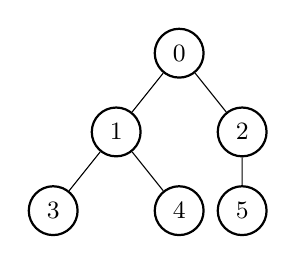
\begin{tikzpicture}[level distance=10mm, sibling distance=16mm]
  \node[gv] {0}
    child {node[gv] {1} child {node[gv] {3}} child {node[gv] {4}}}
    child {node[gv] {2} child {node[gv] {5}}};
\end{tikzpicture}
\end{center}
\end{example}

\topic{八、复杂度与 O 记号}

算法的\term{时间复杂度}是它在输入规模为 $n$（图算法中是 $n$ 与 $m$）时执行的基本步骤数（一次比较、一次赋值、一次加法……）的上界。我们只关心增长的快慢，不关心常数倍。

\begin{definition}\label{def:data-structures:big-o}
设 $f,g$ 是正整数上的非负函数。若存在常数 $C>0$ 与 $n_0$，使 $n\geqslant n_0$ 时 $f(n)\leqslant Cg(n)$，则记 $f=O(g)$。若 $f=O(g)$ 且 $g=O(f)$，记 $f=\Theta(g)$。
\end{definition}

例如 $3n^2+5n+7=O(n^2)$：取 $C=15$，$n_0=1$，因为 $n\geqslant1$ 时 $3n^2+5n+7\leqslant3n^2+5n^2+7n^2$。

数步数的几条规则：
\begin{enumerate}
\item 一串操作依次执行，步数相加；循环执行 $k$ 次、每次 $O(t)$ 步，共 $O(kt)$ 步。
\item 两重循环 \texttt{for i in range(n): for j in range(n):} 共 $n^2$ 次。
\item \emph{对每个顶点扫一遍它的邻接表}：外层 $n$ 次，内层第 $v$ 次是 $d(v)$ 次，共 $\sum_v(1+d(v))=n+2m$ 次，是 $O(n+m)$，而不是 $O(n\cdot\Delta)$ 或 $O(n^2)$。这是后面几乎所有“线性时间”结论的来源。
\item 每次把问题规模减半（$n\to n/2\to n/4\to\cdots$），减到 $1$ 需要 $\log_2n$ 次。
\end{enumerate}

\begin{center}
\begin{tabular}{rrrr}
\toprule
$n$ & $n\log_2n$ & $n^2$ & $2^n$ \\
\midrule
$10$ & $33$ & $100$ & $1024$ \\
$10^3$ & $\approx10^4$ & $10^6$ & $\approx10^{301}$ \\
$10^6$ & $\approx2\times10^7$ & $10^{12}$ & 不可想象 \\
\bottomrule
\end{tabular}
\end{center}

计算机每秒大约做 $10^8$ 到 $10^9$ 次基本操作。$n=10^6$ 时，$O(n\log n)$ 的算法瞬间完成，$O(n^2)$ 的要算几十分钟到几小时，指数时间的算法永远算不完。所以同一个问题，$O(m+n\log n)$ 与 $O(n^2)$ 的区别在大图上是实质的，这就是第~\ref{lec:mst-prim} 讲要引入斐波那契堆的原因。

\topic{小结}

\begin{center}
\begin{tabular}{llll}
\toprule
结构 & 取第 $i$ 个 & 在已知位置插入、删除 & 用途 \\
\midrule
列表 & $O(1)$ & 末尾 $O(1)$，其他 $O(n)$ & 邻接矩阵、各种标记数组 \\
链表 & $O(i)$ & $O(1)$ & 邻接表、欧拉环游的拼接 \\
栈 & 只取栈顶 $O(1)$ & 只在栈顶 $O(1)$ & DFS \\
队列 & 只取队首 $O(1)$ & 队尾进、队首出 $O(1)$ & BFS \\
字典、集合 & 按键 $O(1)$ & 按键 $O(1)$ & 边权、判断成员 \\
双亲数组 & 双亲 $O(1)$ & 改双亲 $O(1)$ & DFS/BFS 树、并查集 \\
\bottomrule
\end{tabular}
\end{center}

\homework{数据结构的练习}[数据结构]

\exercisepart{练习}

\begin{exercises}{A}{数据结构}
\item\label{ex:data-structures:A1} 在例子~\ref{ex:data-structures:linked} 的链表（\texttt{data=[5,3,7,9]}，\texttt{nxt=[-1,3,1,0]}，\texttt{head=2}）上，写一个函数 \texttt{delete\_after(lst,p)} 删去结点 \texttt{p} 后面的那个结点，并写出删去 $3$ 后面的 $9$ 之后 \texttt{nxt} 的值。
\begin{solution}
只需让 \texttt{p} 跳过它的下一个结点，指向下一个的下一个：
\begin{lstlisting}[language=Python]
def delete_after(lst, p):
    q = lst["nxt"][p]            # 要删的结点
    if q != NULL:
        lst["nxt"][p] = lst["nxt"][q]
\end{lstlisting}
$3$ 在结点 $1$，\texttt{q=nxt[1]=3}，\texttt{nxt[1]=nxt[3]=0}，于是 \texttt{nxt=[-1,0,1,0]}。从头走 $2\to1\to0$，链表是 $7\to3\to5$。结点 $3$ 还留在列表里，但已经没有指针指向它，走不到了。
\end{solution}

\item\label{ex:data-structures:A2} 写一个函数 \texttt{reverse(lst)}，把链表的顺序倒过来，只改 \texttt{nxt} 与 \texttt{head}，并说明它是 $O(n)$ 的。
\begin{solution}
从头往后走，把每个结点的 \texttt{nxt} 改指它的前一个结点：
\begin{lstlisting}[language=Python]
def reverse(lst):
    prev, p = NULL, lst["head"]
    while p != NULL:
        q = lst["nxt"][p]       # 先记住下一个，否则改完就找不到了
        lst["nxt"][p] = prev
        prev, p = p, q
    lst["head"] = prev
\end{lstlisting}
在 $7\to3\to5$（结点 $2,1,0$）上：开始 \texttt{prev=-1}，\texttt{p=2}；第一轮 \texttt{q=1}，\texttt{nxt[2]=-1}，\texttt{prev=2}，\texttt{p=1}；第二轮 \texttt{q=0}，\texttt{nxt[1]=2}，\texttt{prev=1}，\texttt{p=0}；第三轮 \texttt{q=-1}，\texttt{nxt[0]=1}，\texttt{prev=0}，\texttt{p=-1}，结束，\texttt{head=0}。得到 $5\to3\to7$。每个结点处理一次，每次 $O(1)$，共 $O(n)$。
\end{solution}

\item\label{ex:data-structures:A3} 用两个栈实现一个队列：进队时放进栈 \texttt{IN}；出队时若栈 \texttt{OUT} 为空，就把 \texttt{IN} 的元素逐个出栈、进栈到 \texttt{OUT}，然后从 \texttt{OUT} 出栈。说明这样取出的顺序确实是先进先出，并说明 $k$ 次操作总共只用 $O(k)$ 步。
\begin{solution}
把 \texttt{IN} 整个倒进 \texttt{OUT} 时，\texttt{IN} 中最早进来的元素在最底下，倒过去之后在 \texttt{OUT} 的最顶上，所以 \texttt{OUT} 从顶到底恰是进队的先后顺序；只有 \texttt{OUT} 空了才再倒，所以 \texttt{OUT} 中的元素总比 \texttt{IN} 中的早进来。每个元素一生中至多进 \texttt{IN} 一次、出 \texttt{IN} 一次、进 \texttt{OUT} 一次、出 \texttt{OUT} 一次，$k$ 次操作涉及至多 $k$ 个元素，总步数 $O(k)$，尽管某一次出队可能要倒很多个元素。这种“单次可能很慢、总数却很少”的分析叫\term{摊还分析}，第~\ref{lec:mst-prim} 讲分析斐波那契堆用的就是它。
\end{solution}

\item\label{ex:data-structures:A4} 求下面三段程序的复杂度（\texttt{adj} 是 $n$ 个顶点、$m$ 条边的图的邻接表）。
\begin{lstlisting}[language=Python,style=frag]
# (a)
for u in range(n):
    for v in range(n):
        if v in adj[u]: c += 1
# (b)
for u in range(n):
    for v in adj[u]:
        c += 1
# (c)
k = n
while k > 1:
    k = k // 2
\end{lstlisting}
\begin{solution}
(a) 两重循环 $n^2$ 次，每次 \texttt{v in adj[u]} 要在列表 \texttt{adj[u]} 中从头找，$O(d(u))$ 步。总共 $\sum_u n\cdot O(1+d(u))=O(n^2+nm)$。若把 \texttt{adj[u]} 换成集合，每次查找 $O(1)$，总共 $O(n^2)$。(b) 规则 3，$O(n+m)$；循环结束时 $c=2m$（无向图每条边在两个端点的表里各出现一次）。(c) 每次 $k$ 减半，约 $\log_2n$ 次，$O(\log n)$。
\end{solution}
\end{exercises}

% !TEX root = ../graph-theory.tex
% =====================================================================
%  组合优化 · 图的存储
% =====================================================================
\lecture{图的存储：邻接矩阵，邻接表（列表版、链表版、顺序数组版），逆邻接表，三元组（边列表），十字链表，邻接多重表，关联矩阵，六种结构的比较}
\label{lec:graph-storage}

同一个图可以有很多种存法。存法决定了两件事：占多少内存，以及几种基本操作（判断 $u,v$ 是否相邻；列出 $v$ 的全部邻点；加一条边；删一条边）各要多少步。一个算法要反复做哪种操作，就该选让这种操作快的存法。这一讲把讲义 2.2 节的六种结构在同几个小图上全部写出来，最后列表比较。

\topic{本讲的例子}

\begin{center}
\begin{tikzpicture}[scale=0.95]
  \begin{scope}
    \node[gv] (0) at (0,1.5) {0}; \node[gv] (1) at (-1.5,0) {1}; \node[gv] (2) at (0,0) {2};
    \node[gv] (3) at (1.5,0) {3}; \node[gv] (4) at (0,-1.5) {4};
    \foreach \a/\b in {0/1,0/2,0/3,1/2,1/4,2/3,2/4,3/4} \draw[ge] (\a) -- (\b);
    \node at (0,-2.3) {$G$：无向图};
  \end{scope}
  \begin{scope}[xshift=4cm,yshift=0.6cm]
    \node[gv] (0) at (0,0) {0}; \node[gv] (1) at (2,0) {1}; \node[gv] (2) at (1,-1.7) {2}; \node[gv] (3) at (3,-1.7) {3};
    \draw[arc] (0) to[bend left=15] (1); \draw[arc] (1) to[bend left=15] (0);
    \draw[arc] (0) -- (2); \draw[arc] (1) to[bend left=15] (2); \draw[arc] (2) to[bend left=15] (1);
    \draw[arc] (1) -- (3); \draw[arc] (3) -- (2);
    \node at (1.5,-2.9) {$D$：有向图};
  \end{scope}
  \begin{scope}[xshift=10cm]
    \node[gv] (0) at (-1.8,0) {0}; \node[gv] (1) at (-0.4,1.3) {1}; \node[gv] (2) at (-0.4,-1.3) {2};
    \node[gv] (3) at (1.5,1.3) {3}; \node[gv] (4) at (1.5,-1.3) {4};
    \foreach \a/\b/\w in {0/1/1,0/2/2,1/2/2,1/3/4,2/4/4,3/4/2} \draw[ge] (\a) -- node[wt] {\w} (\b);
    \draw[ge] (1) -- node[wt,pos=0.3] {3} (4); \draw[ge] (2) -- node[wt,pos=0.3] {4} (3);
    \node at (0,-2.3) {$N$：带权无向图};
  \end{scope}
\end{tikzpicture}
\end{center}

\begin{itemize}
\item $G$（讲义图 1.1）：$5$ 个顶点、$8$ 条边，\texttt{G\_edges=[(0,1),(0,2),(0,3),(1,2),(1,4),(2,3),(2,4),(3,4)]}。
\item $D$（讲义图 1.2）：$4$ 个顶点、$7$ 条弧，\texttt{D\_arcs=[(0,1),(0,2),(1,0),(1,2),(1,3),(2,1),(3,2)]}，$(u,v)$ 表示弧 $u\to v$。
\item $N$（讲义图 1.3）：$5$ 个顶点、$8$ 条带权边，\texttt{N\_edges=[(0,1,1),(0,2,2),(1,2,2),(1,3,4),(1,4,3),(2,3,4),(2,4,4),(3,4,2)]}，$(u,v,c)$ 表示边 $uv$ 的权为 $c$。
\end{itemize}

我们假设图一开始是以“边的列表”给出的（这也是读入数据时最常见的形式），然后把它转成各种结构。

\begin{lstlisting}[language=Python]
INF = float('inf')
NULL = -1
G_edges = [(0, 1), (0, 2), (0, 3), (1, 2), (1, 4), (2, 3), (2, 4), (3, 4)]
D_arcs = [(0, 1), (0, 2), (1, 0), (1, 2), (1, 3), (2, 1), (3, 2)]
N_edges = [(0, 1, 1), (0, 2, 2), (1, 2, 2), (1, 3, 4), (1, 4, 3),
           (2, 3, 4), (2, 4, 4), (3, 4, 2)]
\end{lstlisting}

\topic{一、邻接矩阵}

$n\times n$ 的表 $A$，$A[u][v]=1$ 当且仅当 $uv$ 是边（有向图中：$u\to v$ 是弧）。带权时 $A[u][v]$ 存权，没有边的位置存 $0$ 或 $\infty$，取哪个看问题：求最短路、最小树时存 $\infty$（“不能走”），求最大权时存 $0$。

\begin{lstlisting}[language=Python]
def adjacency_matrix(n, edges, directed=False):
    A = [[0] * n for _ in range(n)]
    for u, v in edges:
        A[u][v] = 1
        if not directed:          # 无向边要填两个对称的位置
            A[v][u] = 1
    return A

def weighted_matrix(n, edges, none=INF):
    W = [[none] * n for _ in range(n)]
    for u, v, c in edges:
        W[u][v] = W[v][u] = c
    return W
\end{lstlisting}

对三个例子：
\[
A(G)=\begin{pmatrix}0&1&1&1&0\\1&0&1&0&1\\1&1&0&1&1\\1&0&1&0&1\\0&1&1&1&0\end{pmatrix},\quad
A(D)=\begin{pmatrix}0&1&1&0\\1&0&1&1\\0&1&0&0\\0&0&1&0\end{pmatrix},
\]
\[
W(N)=\begin{pmatrix}\infty&1&2&\infty&\infty\\1&\infty&2&4&3\\2&2&\infty&4&4\\\infty&4&4&\infty&2\\\infty&3&4&2&\infty\end{pmatrix}.
\]
无向图的矩阵对称，第 $v$ 行中 $1$ 的个数是 $d(v)$；有向图的第 $v$ 行之和是出度，第 $v$ 列之和是入度。

\emph{代价。}判断 $u,v$ 是否相邻：看 \texttt{A[u][v]}，$O(1)$。加边、删边：改一格，$O(1)$。列出 $v$ 的邻点：要扫描整个第 $v$ 行，$O(n)$，不论 $v$ 有几个邻点。内存 $n^2$ 格。边很少的图（比如 $m\approx3n$）大部分格子是 $0$，既浪费内存，也让“扫一遍所有邻点”的算法变成 $O(n^2)$。

\topic{二、邻接表}

给每个顶点一张表，列出它的邻点。最直接的 Python 写法是“列表的列表”：

\begin{lstlisting}[language=Python]
def adjacency_list(n, edges, directed=False):
    adj = [[] for _ in range(n)]
    for u, v in edges:
        adj[u].append(v)
        if not directed:
            adj[v].append(u)
    return adj
\end{lstlisting}

\texttt{adjacency\_list(5,G\_edges)} 得到 \texttt{[[1,2,3],[0,2,4],[0,1,3,4],[0,2,4],[1,2,3]]}；\texttt{adjacency\_list(4,D\_arcs,True)} 得到 \texttt{[[1,2],[0,2,3],[1],[2]]}。带权时表里存 \texttt{(邻点,权)}。

\emph{代价。}列出 $v$ 的邻点：$O(d(v))$，这是邻接表最大的优点。对所有顶点各列一遍，共 $O(n+m)$（第~\ref{lec:data-structures} 讲复杂度规则 3）。判断 $u,v$ 是否相邻：要在 \texttt{adj[u]} 里找，$O(d(u))$。内存 $n+2m$（无向）或 $n+m$（有向）。

\topic{二之一、讲义的写法：点表加边表（链表）}

讲义把邻接表描述为两部分：\emph{点表}是长为 $n$ 的数组，第 $v$ 格存 $v$ 的边表的\emph{头指针}；\emph{边表}是每个顶点一条单链表，每个结点存一个邻点（\texttt{data}）、可能还有权，以及下一个结点（\texttt{next}）。按第~\ref{lec:data-structures} 讲的办法，用数组模拟：\texttt{head[v]} 是点表，\texttt{data}、\texttt{nxt} 存所有结点。

\begin{lstlisting}[language=Python]
def linked_adjacency(n, arcs):
    """有向图的链表式邻接表：点表 head，边表结点的 data 与 nxt。"""
    head = [NULL] * n
    data, nxt = [], []
    for u, v in arcs:
        k = len(data)            # 新结点的编号
        data.append(v)
        nxt.append(head[u])      # 插在 u 的边表最前面
        head[u] = k
    return head, data, nxt

def neighbours_linked(head, data, nxt, u):
    out, p = [], head[u]
    while p != NULL:             # 讲义写作 while p != NULL: ... p = p.next
        out.append(data[p])
        p = nxt[p]
    return out
\end{lstlisting}

对 $D$ 逐条插入弧，每条弧占一个结点，结点编号就是弧在 \texttt{D\_arcs} 中的位置：

\begin{center}
\begin{tabular}{cccccc}
\toprule
第几条弧 & 弧 & 结点 $k$ & \texttt{data[k]} & \texttt{nxt[k]}（$u$ 原来的头） & 之后的 \texttt{head} \\
\midrule
1 & $0\to1$ & 0 & 1 & $-1$ & \texttt{[0,-1,-1,-1]} \\
2 & $0\to2$ & 1 & 2 & 0 & \texttt{[1,-1,-1,-1]} \\
3 & $1\to0$ & 2 & 0 & $-1$ & \texttt{[1,2,-1,-1]} \\
4 & $1\to2$ & 3 & 2 & 2 & \texttt{[1,3,-1,-1]} \\
5 & $1\to3$ & 4 & 3 & 3 & \texttt{[1,4,-1,-1]} \\
6 & $2\to1$ & 5 & 1 & $-1$ & \texttt{[1,4,5,-1]} \\
7 & $3\to2$ & 6 & 2 & $-1$ & \texttt{[1,4,5,6]} \\
\bottomrule
\end{tabular}
\end{center}

最后 \texttt{head=[1,4,5,6]}，\texttt{data=[1,2,0,2,3,1,2]}，\texttt{nxt=[-1,0,-1,2,3,-1,-1]}。列出顶点 $1$ 的出邻点：\texttt{p=head[1]=4}，\texttt{data[4]=3}；\texttt{p=nxt[4]=3}，\texttt{data[3]=2}；\texttt{p=nxt[3]=2}，\texttt{data[2]=0}；\texttt{p=nxt[2]=-1}，停。得到 $3,2,0$。顺序与插入顺序相反，因为每次都插在最前面；对图算法来说邻点的顺序无关紧要。

\begin{center}
\begin{tikzpicture}
  \foreach \v in {0,...,3} { \node[cell] (h\v) at (0,-\v*0.8) {\v}; }
  \node[idx] at (0,0.55) {点表};
  % vertex 0: nodes 1 -> 0
  \node[cell] (a1) at (1.8,0) {2}; \node[cell] (b1) at (2.55,0) {};
  \node[cell] (a0) at (3.9,0) {1}; \node[cell] (b0) at (4.65,0) {$\wedge$};
  \draw[ptr] (h0) -- (a1); \draw[ptr] (b1.center) -- (a0);
  % vertex 1: 4 -> 3 -> 2
  \node[cell] (a4) at (1.8,-0.8) {3}; \node[cell] (b4) at (2.55,-0.8) {};
  \node[cell] (a3) at (3.9,-0.8) {2}; \node[cell] (b3) at (4.65,-0.8) {};
  \node[cell] (a2) at (6.0,-0.8) {0}; \node[cell] (b2) at (6.75,-0.8) {$\wedge$};
  \draw[ptr] (h1) -- (a4); \draw[ptr] (b4.center) -- (a3); \draw[ptr] (b3.center) -- (a2);
  % vertex 2: 5
  \node[cell] (a5) at (1.8,-1.6) {1}; \node[cell] (b5) at (2.55,-1.6) {$\wedge$};
  \draw[ptr] (h2) -- (a5);
  % vertex 3: 6
  \node[cell] (a6) at (1.8,-2.4) {2}; \node[cell] (b6) at (2.55,-2.4) {$\wedge$};
  \draw[ptr] (h3) -- (a6);
  \node[idx] at (2.17,0.55) {data \ next};
\end{tikzpicture}
\end{center}

链表版的好处是加边只需 $O(1)$ 地插入一个结点；删去一条已知前驱结点的边也是 $O(1)$。Python 的列表也能在末尾 $O(1)$ 地加边，所以本书的程序一般直接用 \texttt{adj[u].append(v)}；需要“逐个往后取下一个邻点、并记住取到了哪里”的算法（DFS 的非递归写法、欧拉环游），本书用一个下标 \texttt{cur[u]} 记住 \texttt{adj[u]} 中下一个要看的位置，它的作用与讲义中“把 \texttt{adj[u]} 指针移到 \texttt{adj[u].next}”完全相同。

\topic{二之二、讲义的顺序数组版（压缩行存储）}

讲义还给出一种只用两个数组的邻接表：\texttt{Edge} 把 $0$ 号顶点的邻点、$1$ 号顶点的邻点、……依次连续地排在一起；\texttt{Vertex[v]} 记 $v$ 的邻点从 \texttt{Edge} 的哪一格开始，\texttt{Vertex[n]} 是 \texttt{Edge} 的总长。于是 $v$ 的邻点是 \texttt{Edge[Vertex[v]:Vertex[v+1]]}。这种结构在数值计算里叫 CSR（compressed sparse row）。

\begin{lstlisting}[language=Python]
def csr(n, edges):
    """无向图的顺序数组邻接表 (Vertex, Edge)。"""
    deg = [0] * n
    for u, v in edges:                # 第一遍：数度数
        deg[u] += 1
        deg[v] += 1
    Vertex = [0] * (n + 1)
    for v in range(n):                # 前缀和：v 的邻点从哪一格开始
        Vertex[v + 1] = Vertex[v] + deg[v]
    Edge = [0] * Vertex[n]
    pos = Vertex[:n]                  # pos[v]：v 的下一个邻点该填在哪一格
    for u, v in edges:                # 第二遍：把邻点填进去
        Edge[pos[u]] = v
        pos[u] += 1
        Edge[pos[v]] = u
        pos[v] += 1
    return Vertex, Edge
\end{lstlisting}

在 $G$ 上一步一步做：
\begin{enumerate}
\item 度数 \texttt{deg=[3,3,4,3,3]}。
\item 前缀和：\texttt{Vertex[0]=0}，\texttt{Vertex[1]=0+3=3}，\texttt{Vertex[2]=3+3=6}，\texttt{Vertex[3]=6+4=10}，\texttt{Vertex[4]=10+3=13}，\texttt{Vertex[5]=13+3=16}。所以 \texttt{Vertex=[0,3,6,10,13,16]}：顶点 $0$ 占第 $0$–$2$ 格，顶点 $1$ 占第 $3$–$5$ 格，顶点 $2$ 占第 $6$–$9$ 格，顶点 $3$ 占第 $10$–$12$ 格，顶点 $4$ 占第 $13$–$15$ 格。
\item 填数。\texttt{pos=[0,3,6,10,13]}。边 $(0,1)$：\texttt{Edge[0]=1}，\texttt{Edge[3]=0}，\texttt{pos=[1,4,6,10,13]}。边 $(0,2)$：\texttt{Edge[1]=2}，\texttt{Edge[6]=0}。边 $(0,3)$：\texttt{Edge[2]=3}，\texttt{Edge[10]=0}。边 $(1,2)$：\texttt{Edge[4]=2}，\texttt{Edge[7]=1}。边 $(1,4)$：\texttt{Edge[5]=4}，\texttt{Edge[13]=1}。边 $(2,3)$：\texttt{Edge[8]=3}，\texttt{Edge[11]=2}。边 $(2,4)$：\texttt{Edge[9]=4}，\texttt{Edge[14]=2}。边 $(3,4)$：\texttt{Edge[12]=4}，\texttt{Edge[15]=3}。
\end{enumerate}
结果 \texttt{Edge=[1,2,3,0,2,4,0,1,3,4,0,2,4,1,2,3]}，与讲义的数组（讲义从 $1$ 编号，每个数大 $1$）一致。顶点 $2$ 的邻点是 \texttt{Edge[6:10]=[0,1,3,4]}。

\begin{center}
\begin{tikzpicture}
  \foreach \v [count=\i from 0] in {0,3,6,10,13,16} \node[cell] (V\i) at (\i*0.8,0) {\v};
  \node[font=\small] at (-1.1,0) {\texttt{Vertex}};
  \foreach \i in {0,...,5} \node[idx] at (\i*0.8,0.5) {\i};
  \foreach \v [count=\i from 0] in {1,2,3,0,2,4,0,1,3,4,0,2,4,1,2,3} \node[cell] (E\i) at (\i*0.62-0.5,-1.6) {\v};
  \foreach \i in {6,7,8,9} \node[cellh] at (\i*0.62-0.5,-1.6) {};
  \foreach \v [count=\i from 6] in {0,1,3,4} \node[font=\small\ttfamily] at (\i*0.62-0.5,-1.6) {\v};
  \node[font=\small] at (-1.6,-1.6) {\texttt{Edge}};
  \foreach \i in {0,...,15} \node[idx] at (\i*0.62-0.5,-2.1) {\i};
  \draw[ptr] (V2.south) -- (E6.north); \draw[ptr] (V3.south) -- (E10.north);
\end{tikzpicture}
\end{center}

\emph{代价。}内存 $n+1+2m$，没有指针，取邻点和列表版一样快。但加边、删边要挪动大段数组，所以只适合图建好之后不再改变的场合。

\topic{二之三、逆邻接表}

有向图的邻接表只存出邻点。有些算法要“反着走”（强连通分支算法的第二步要找“能到达 $w$ 的点”），这时再存一份\emph{逆邻接表}，即把所有弧反向之后的邻接表，它列出每个顶点的入邻点。

\begin{lstlisting}[language=Python]
def reverse_adjacency(n, arcs):
    radj = [[] for _ in range(n)]
    for u, v in arcs:
        radj[v].append(u)        # 弧 u->v 记在 v 的表里
    return radj
\end{lstlisting}

$D$ 的逆邻接表是 \texttt{[[1],[0,2],[0,1,3],[1]]}：例如顶点 $2$ 的入邻点是 $0,1,3$。

\topic{三、三元组（边列表）}

最朴素的存法：一个列表，每个元素是一条边 $(u,v,c)$，再记下 $n$ 与 $m$。讲义称每个元素为一个“三元组”，三个分量叫行号、列号与权，因为它们正是邻接矩阵中一个非零元的位置与数值。不带权时就是边列表，例如 \texttt{G\_edges}。

\emph{代价。}内存 $3m$。列出某个顶点的邻点要扫描全部 $m$ 条边。它的用处是可以\emph{按权排序}：Kruskal 算法第一步就是把边按权从小到大排好（第~\ref{lec:mst-kruskal} 讲）。

\begin{lstlisting}[language=Python,style=frag]
sorted(N_edges, key=lambda e: e[2])   # 按第 3 个分量（权）排序
# [(0,1,1), (0,2,2), (1,2,2), (3,4,2), (1,4,3), (1,3,4), (2,3,4), (2,4,4)]
\end{lstlisting}

\topic{四、十字链表（有向图）}

想同时快速地列出出邻点和入邻点，可以把邻接表与逆邻接表合在一起：每条弧只存\emph{一个}结点，但这个结点同时挂在两条链表上，一条是它的尾的出弧链表（矩阵的“行”），一条是它的头的入弧链表（矩阵的“列”），像一个十字。

每条弧 $k$ 存五项：尾 \texttt{tail[k]}、头 \texttt{head[k]}、权 \texttt{w[k]}、同一行的下一条弧 \texttt{tnext[k]}（讲义的 \texttt{linnext}）、同一列的下一条弧 \texttt{hnext[k]}（讲义的 \texttt{colnext}）。每个顶点存两个头指针：\texttt{firstout[v]}（讲义的 \texttt{firstout}，第一条出弧）与 \texttt{firstin[v]}（第一条入弧）。

\begin{lstlisting}[language=Python]
def orthogonal_list(n, warcs):
    """warcs: [(u, v, c)]。返回十字链表的七个数组。"""
    firstout, firstin = [NULL] * n, [NULL] * n
    tail, head, w, tnext, hnext = [], [], [], [], []
    for u, v, c in warcs:
        k = len(tail)
        tail.append(u); head.append(v); w.append(c)
        tnext.append(firstout[u]); firstout[u] = k   # 挂到 u 的出弧链表最前面
        hnext.append(firstin[v]);  firstin[v] = k    # 挂到 v 的入弧链表最前面
    return firstout, firstin, tail, head, w, tnext, hnext

def out_arcs(L, u):
    firstout, firstin, tail, head, w, tnext, hnext = L
    out, k = [], firstout[u]
    while k != NULL:
        out.append((head[k], w[k]))
        k = tnext[k]
    return out

def in_arcs(L, v):
    firstout, firstin, tail, head, w, tnext, hnext = L
    out, k = [], firstin[v]
    while k != NULL:
        out.append((tail[k], w[k]))
        k = hnext[k]
    return out
\end{lstlisting}

例子（讲义图 1.4）的邻接矩阵是
\[
\begin{pmatrix}0&8&7&0\\0&0&0&0\\6&0&0&8\\5&6&9&0\end{pmatrix},
\]
即七条带权的弧：

\begin{lstlisting}[language=Python]
O_arcs = [(0, 1, 8), (0, 2, 7), (2, 0, 6), (2, 3, 8), (3, 0, 5), (3, 1, 6), (3, 2, 9)]
\end{lstlisting}

按顺序插入七条弧，得到的数组：

\begin{center}
\begin{tabular}{cccccc}
\toprule
弧 $k$ & \texttt{tail} & \texttt{head} & \texttt{w} & \texttt{tnext}（同尾的下一条） & \texttt{hnext}（同头的下一条） \\
\midrule
0 & 0 & 1 & 8 & $-1$ & $-1$ \\
1 & 0 & 2 & 7 & 0 & $-1$ \\
2 & 2 & 0 & 6 & $-1$ & $-1$ \\
3 & 2 & 3 & 8 & 2 & $-1$ \\
4 & 3 & 0 & 5 & $-1$ & 2 \\
5 & 3 & 1 & 6 & 4 & 0 \\
6 & 3 & 2 & 9 & 5 & 1 \\
\bottomrule
\end{tabular}
\qquad
\begin{tabular}{ccc}
\toprule
顶点 & \texttt{firstout} & \texttt{firstin} \\
\midrule
0 & 1 & 4 \\
1 & $-1$ & 5 \\
2 & 3 & 6 \\
3 & 6 & 3 \\
\bottomrule
\end{tabular}
\end{center}

例如 \texttt{hnext[4]=2}：插入弧 $4$（$3\to0$）时，顶点 $0$ 的入弧链表原来以弧 $2$（$2\to0$）开头，弧 $4$ 插到它前面。列出顶点 $3$ 的出弧：\texttt{k=firstout[3]=6}（$3\to2$，权 $9$），\texttt{k=tnext[6]=5}（$3\to1$，权 $6$），\texttt{k=tnext[5]=4}（$3\to0$，权 $5$），\texttt{k=tnext[4]=-1}，停。列出顶点 $0$ 的入弧：\texttt{k=firstin[0]=4}（来自 $3$），\texttt{k=hnext[4]=2}（来自 $2$），\texttt{k=hnext[2]=-1}，停。

\emph{代价。}出弧、入弧都能按 $O(\text{个数})$ 列出，内存 $2n+5m$。它是“邻接矩阵的稀疏存储”：只存非零元，并把同一行、同一列的非零元各串成链。

\topic{五、邻接多重表（无向图）}

无向图的邻接表中，每条边 $uv$ 出现两次（在 $u$ 的表里一次，在 $v$ 的表里一次）。求欧拉环游时要标记“这条边已经走过”，若边存了两份，就要同时找到并标记两份，很麻烦。邻接多重表让每条边只存一个结点，这个结点同时挂在两个端点的链表上：边 $k$ 存端点 \texttt{I[k]}、\texttt{J[k]}、权 \texttt{W[k]}，以及“在 \texttt{I[k]} 的链表上的下一条边” \texttt{inext[k]}、“在 \texttt{J[k]} 的链表上的下一条边” \texttt{jnext[k]}；顶点 $v$ 存 \texttt{first[v]}。

\begin{lstlisting}[language=Python]
def multilist(n, wedges):
    first = [NULL] * n
    I, J, W, inext, jnext = [], [], [], [], []
    for u, v, c in wedges:
        k = len(I)
        I.append(u); J.append(v); W.append(c)
        inext.append(first[u]); first[u] = k     # 挂到 u 的链表最前面
        jnext.append(first[v]); first[v] = k     # 也挂到 v 的链表最前面
    return first, I, J, W, inext, jnext

def edges_at(M, v):
    """v 关联的全部边的编号。"""
    first, I, J, W, inext, jnext = M
    out, e = [], first[v]
    while e != NULL:
        out.append(e)
        e = inext[e] if I[e] == v else jnext[e]  # v 是这条边的哪一端，就走哪一个 next
    return out
\end{lstlisting}

对 $N$：

\begin{center}
\begin{tabular}{ccccccc}
\toprule
边 $k$ & \texttt{I} & \texttt{J} & \texttt{W} & \texttt{inext} & \texttt{jnext} \\
\midrule
0 & 0 & 1 & 1 & $-1$ & $-1$ \\
1 & 0 & 2 & 2 & 0 & $-1$ \\
2 & 1 & 2 & 2 & 0 & 1 \\
3 & 1 & 3 & 4 & 2 & $-1$ \\
4 & 1 & 4 & 3 & 3 & $-1$ \\
5 & 2 & 3 & 4 & 2 & 3 \\
6 & 2 & 4 & 4 & 5 & 4 \\
7 & 3 & 4 & 2 & 5 & 6 \\
\bottomrule
\end{tabular}
\qquad \texttt{first=[1,4,6,7,7]}
\end{center}

列出顶点 $2$ 关联的边：\texttt{e=first[2]=6}，\texttt{I[6]=2}，所以下一条是 \texttt{inext[6]=5}；\texttt{I[5]=2}，下一条 \texttt{inext[5]=2}；边 $2$ 是 $(1,2)$，$2$ 是 \texttt{J} 端，下一条 \texttt{jnext[2]=1}；边 $1$ 是 $(0,2)$，$2$ 是 \texttt{J} 端，下一条 \texttt{jnext[1]=-1}，停。得到边 $6,5,2,1$，即 $24,23,12,02$。

\topic{六、关联矩阵}

$n\times m$ 的矩阵 $B$，行对应顶点，列对应边。无向图中 $B[v][k]=1$ 当且仅当 $v$ 是边 $k$ 的端点；有向图中 $B[v][k]=1$ 若 $v$ 是弧 $k$ 的尾，$-1$ 若是头，否则 $0$。每列恰有两个非零元。

\begin{lstlisting}[language=Python]
def incidence_matrix(n, edges, directed=False):
    B = [[0] * len(edges) for _ in range(n)]
    for k, (u, v) in enumerate(edges):   # enumerate 同时给出编号 k 与边 (u, v)
        B[u][k] = 1
        B[v][k] = -1 if directed else 1
    return B
\end{lstlisting}

$G$ 的关联矩阵（列按 \texttt{G\_edges} 的顺序：$01,02,03,12,14,23,24,34$）：
\[
B(G)=\begin{pmatrix}
1&1&1&0&0&0&0&0\\
1&0&0&1&1&0&0&0\\
0&1&0&1&0&1&1&0\\
0&0&1&0&0&1&0&1\\
0&0&0&0&1&0&1&1
\end{pmatrix}.
\]
关联矩阵有 $nm$ 格，几乎全是 $0$，不用来写程序。它的用处在理论上：有向图的关联矩阵是\emph{全单模}的（每个方子式都是 $0$ 或 $\pm1$），这是网络流、最短路等问题的线性规划有整数最优解的原因，以后会用到。

\topic{七、比较}

\begin{center}
\small
\begin{tabular}{lccccc}
\toprule
结构 & 内存 & $u,v$ 是否相邻 & 列出 $N^+(v)$ & 列出 $N^-(v)$ & 加边 \\
\midrule
邻接矩阵 & $n^2$ & $O(1)$ & $O(n)$ & $O(n)$ & $O(1)$ \\
邻接表（列表、链表） & $n+m$ & $O(d^+(u))$ & $O(d^+(v))$ & $O(m)$ & $O(1)$ \\
邻接表 $+$ 逆邻接表 & $n+2m$ & $O(d^+(u))$ & $O(d^+(v))$ & $O(d^-(v))$ & $O(1)$ \\
顺序数组（CSR） & $n+m$ & $O(d^+(u))$ & $O(d^+(v))$ & $O(m)$ & $O(n+m)$ \\
三元组（边列表） & $3m$ & $O(m)$ & $O(m)$ & $O(m)$ & $O(1)$ \\
十字链表 & $2n+5m$ & $O(d^+(u))$ & $O(d^+(v))$ & $O(d^-(v))$ & $O(1)$ \\
邻接多重表（无向） & $n+5m$ & $O(d(u))$ & $O(d(v))$ & — & $O(1)$ \\
关联矩阵 & $nm$ & $O(m)$ & $O(m)$ & $O(m)$ & — \\
\bottomrule
\end{tabular}
\end{center}

（无向图把 $d^+$、$d^-$ 都读作 $d$，邻接表的内存是 $n+2m$。）选择的原则：
\begin{itemize}
\item 算法的主要工作是“对每个顶点扫一遍它的邻点”（遍历、强连通分支、拓扑排序、Prim）：用邻接表，得到 $O(n+m)$ 的时间。
\item 要大量回答“$u,v$ 是否相邻”，或图很稠密（$m$ 接近 $n^2$）：用邻接矩阵。
\item 要按权排序所有边：用三元组。
\item 有向图要双向走：邻接表加逆邻接表，或十字链表。
\item 无向图要给边打标记：邻接多重表，或者给每条边一个编号、在邻接表里存编号（第~\ref{lec:euler-tours} 讲就这样做）。
\end{itemize}

\homework{图的存储的练习}[图的存储]

\exercisepart{练习}

\begin{exercises}{A}{图的存储}
\item\label{ex:graph-storage:A1} 写出把邻接矩阵转成邻接表、以及把邻接表转成邻接矩阵的函数，并说明各自的复杂度。
\begin{solution}
\begin{lstlisting}[language=Python]
def matrix_to_list(A):
    n = len(A)
    return [[v for v in range(n) if A[u][v]] for u in range(n)]

def list_to_matrix(adj):
    n = len(adj)
    A = [[0] * n for _ in range(n)]
    for u in range(n):
        for v in adj[u]:
            A[u][v] = 1
    return A
\end{lstlisting}
第一个要看矩阵的每一格，$O(n^2)$。第二个造全零矩阵要 $O(n^2)$，填数只要 $O(n+m)$，合计 $O(n^2)$。所以矩阵与表之间的转换都是 $O(n^2)$，转换本身就可能比后面要跑的线性算法慢。
\end{solution}

\item\label{ex:graph-storage:A2} 有向图 $D$ 以邻接表给出。写一个 $O(n+m)$ 的函数求它的逆邻接表，只用 \texttt{adj}，不用弧的列表。
\begin{solution}
\begin{lstlisting}[language=Python]
def reverse_of(adj):
    n = len(adj)
    radj = [[] for _ in range(n)]
    for u in range(n):
        for v in adj[u]:          # 弧 u->v
            radj[v].append(u)
    return radj
\end{lstlisting}
两重循环共执行 $\sum_u(1+d^+(u))=n+m$ 次。对 $D$ 的邻接表 \texttt{[[1,2],[0,2,3],[1],[2]]} 得到 \texttt{[[1],[0,2],[0,1,3],[1]]}。
\end{solution}

\item\label{ex:graph-storage:A3} 用 \texttt{csr} 得到的 $(\texttt{Vertex},\texttt{Edge})$，写一个函数在 $O(\log d(u))$ 时间内判断 $u,v$ 是否相邻（提示：先把每个顶点的邻点排好序）。
\begin{solution}
先对每段 \texttt{Edge[Vertex[u]:Vertex[u+1]]} 排序（总共 $O(m\log n)$，只做一次）。查询时在这一段里二分查找：
\begin{lstlisting}[language=Python]
def sort_csr(Vertex, Edge):
    for u in range(len(Vertex) - 1):
        Edge[Vertex[u]:Vertex[u + 1]] = sorted(Edge[Vertex[u]:Vertex[u + 1]])

def adjacent_csr(Vertex, Edge, u, v):
    lo, hi = Vertex[u], Vertex[u + 1]      # 在 Edge[lo:hi] 中找 v
    while lo < hi:
        mid = (lo + hi) // 2
        if Edge[mid] < v:
            lo = mid + 1
        else:
            hi = mid
    return lo < Vertex[u + 1] and Edge[lo] == v
\end{lstlisting}
每轮把区间 $[lo,hi)$ 减半，$O(\log d(u))$ 轮。循环结束时 $lo$ 是第一个 $\geqslant v$ 的位置。
\end{solution}

\item\label{ex:graph-storage:A4} 证明：有向图的关联矩阵 $B$ 的每一列之和为 $0$，所以 $B$ 的秩至多为 $n-1$；并说明当底图连通时秩恰为 $n-1$。
\begin{solution}
每列恰有一个 $1$（尾）和一个 $-1$（头），列和为 $0$，即全 $1$ 行向量 $\mathbf 1^\top$ 满足 $\mathbf1^\top B=0$，所以 $B$ 的行向量线性相关，秩 $\leqslant n-1$。设底图连通，$y^\top B=0$，则对每条弧 $u\to v$ 有 $y_u-y_v=0$；沿底图中的路传递，所有 $y_v$ 相等，所以左零空间是一维的，秩为 $n-1$。
\end{solution}
\end{exercises}

% !TEX root = ../graph-theory.tex
% =====================================================================
%  组合优化 · 图的遍历
% =====================================================================
\lecture{图的遍历：通用的扫描算法及其正确性，深度优先搜索（栈），广度优先搜索（队列），邻接矩阵与邻接表下的实现与复杂度，连通分支，二部图的判定与奇圈的找出}
\label{lec:traversal}

遍历是从一个顶点 $s$ 出发，沿着边把能到达的顶点都访问一遍。几乎所有图算法都以遍历为骨架：求连通分支、判断二部图、求强连通分支、拓扑排序、找欧拉环游、求 st-编号，都是在遍历的过程中顺便记录一些信息。所以这一讲把遍历讲透：先讲一个通用的算法并证明它对，然后看“从哪里继续”的两种选法（栈与队列）分别得到什么，最后分析它在两种存储结构下要花多少时间。

\topic{一、通用的扫描算法}

算法维护三样东西（讲义算法 2.1）：
\begin{itemize}
\item $R$：已经到达的顶点；
\item $Q$：已经到达、但可能还有边没检查过的顶点（“待处理”）；
\item $T$：搜索树的边，每个新顶点 $w$ 进入 $R$ 时，记下是从哪个顶点 $v$ 走过来的。
\end{itemize}

\begin{enumerate}
\item 开始：$R=Q=\{s\}$，$T=\varnothing$。
\item 若 $Q=\varnothing$，停止。否则从 $Q$ 中\emph{选}一个顶点 $v$。
\item 若 $v$ 有不在 $R$ 中的邻点 $w$：把 $w$ 放进 $R$ 和 $Q$，把边 $vw$ 放进 $T$。否则把 $v$ 从 $Q$ 中删去。回到第 2 步。
\end{enumerate}

\begin{theorem}\label{thm:traversal:scan}
无论第 2 步怎样选 $v$，算法都会停止；停止时 $R$ 恰是从 $s$ 可到达的顶点集，$(R,T)$ 是一棵树（有向图中是以 $s$ 为根的分支）。
\end{theorem}
\begin{proof}
\emph{停止。}第 3 步每执行一次，或者 $R$ 增加一个顶点（至多 $n-1$ 次），或者 $Q$ 减少一个顶点；每个顶点只进 $Q$ 一次（进 $Q$ 时同时进 $R$，而进 $R$ 的顶点不再进），所以也只出 $Q$ 一次。第 3 步至多执行 $2n$ 次。

\emph{$(R,T)$ 是树。}每加入一个新顶点 $w$，恰好同时加入一条边 $vw$，$v$ 已在 $R$ 中。所以始终有 $\abs T=\abs R-1$，且 $(R,T)$ 连通；由树的等价刻画（讲义第 1 章定理 1.8），它是树。有向图中每个非 $s$ 的顶点恰有一条进入它的树弧，是分支。

\emph{$R$ 是可达集。}$R$ 中的顶点显然可达。设 $x$ 可达但 $x\notin R$。取一条 $(s,x)$-路，它从 $R$ 出发，最终离开 $R$，所以有一条边 $vw$，$v\in R$，$w\notin R$。$v$ 进过 $Q$，而 $v$ 离开 $Q$ 的条件是 $v$ 没有不在 $R$ 中的邻点；但 $w$ 一直不在 $R$ 中，矛盾。
\end{proof}

第 2 步“选哪个 $v$”留给我们决定。两种选法：
\begin{itemize}
\item 总选\emph{最后}进入 $Q$ 的顶点：$Q$ 是栈，得到\term{深度优先搜索}（DFS）。它一有新顶点就从新顶点继续往前走，走不动了才退回来。
\item 总选\emph{最先}进入 $Q$ 的顶点：$Q$ 是队列，得到\term{广度优先搜索}（BFS）。它先把 $s$ 的邻点都找到，再找邻点的邻点，一层一层地往外推。
\end{itemize}

两种算法都用一个双亲数组 \texttt{tree} 同时记录 $R$ 与 $T$：\texttt{tree[v]}$=-2$ 表示 $v\notin R$，$-1$ 表示 $v=s$ 是根，否则 \texttt{tree[v]} 是 $v$ 在搜索树中的双亲（即边 $(\texttt{tree[v]},v)\in T$）。

\topic{二、深度优先搜索}

“$v$ 有没有不在 $R$ 中的邻点”不能每次都从 \texttt{adj[v]} 的开头重新找，否则同一条边会被反复检查。所以给每个顶点一个下标 \texttt{cur[v]}，表示 \texttt{adj[v]} 中前 \texttt{cur[v]} 个邻点已经看过了，下次从第 \texttt{cur[v]} 个接着看。讲义中邻接表版的 DFS 把 \texttt{visited[i]} 设为边表的头指针、每看一个邻点就令 \texttt{visited[i]=visited[i].next}，是同一个意思。

\begin{lstlisting}[language=Python]
def dfs(adj, s):
    """从 s 出发的深度优先搜索，返回双亲数组 tree。"""
    n = len(adj)
    tree = [-2] * n          # -2：还没到达
    cur = [0] * n            # cur[v]：adj[v] 中下一个要看的位置
    tree[s] = -1             # s 是根
    stack = [s]
    while stack:
        u = stack[-1]                    # 看栈顶，不取走
        if cur[u] < len(adj[u]):         # u 还有没看过的邻点
            v = adj[u][cur[u]]
            cur[u] += 1
            if tree[v] == -2:            # v 是新顶点
                tree[v] = u
                stack.append(v)          # 从 v 继续往前走
        else:                            # u 的邻点都看过了
            stack.pop()                  # 退回到 u 的上一个顶点
    return tree
\end{lstlisting}

\begin{example}\label{ex:traversal:dfs}
在上一讲的图 $G$ 上从 $s=0$ 做 DFS，\texttt{adj=[[1,2,3],[0,2,4],[0,1,3,4],[0,2,4],[1,2,3]]}。下表每一行是 \texttt{while} 循环的一轮：

\begin{center}
\small
\begin{tabular}{rllll}
\toprule
轮 & 栈顶 $u$ & 这一轮看的邻点 & 动作 & 之后的栈 \\
\midrule
0 & & & 初始化，\texttt{tree=[-1,-2,-2,-2,-2]} & \texttt{[0]} \\
1 & 0 & \texttt{adj[0][0]=1} & 新顶点，\texttt{tree[1]=0}，进栈 & \texttt{[0,1]} \\
2 & 1 & \texttt{adj[1][0]=0} & 已到达，跳过 & \texttt{[0,1]} \\
3 & 1 & \texttt{adj[1][1]=2} & 新顶点，\texttt{tree[2]=1}，进栈 & \texttt{[0,1,2]} \\
4 & 2 & \texttt{adj[2][0]=0} & 已到达 & \texttt{[0,1,2]} \\
5 & 2 & \texttt{adj[2][1]=1} & 已到达 & \texttt{[0,1,2]} \\
6 & 2 & \texttt{adj[2][2]=3} & 新顶点，\texttt{tree[3]=2}，进栈 & \texttt{[0,1,2,3]} \\
7 & 3 & \texttt{adj[3][0]=0} & 已到达 & \texttt{[0,1,2,3]} \\
8 & 3 & \texttt{adj[3][1]=2} & 已到达 & \texttt{[0,1,2,3]} \\
9 & 3 & \texttt{adj[3][2]=4} & 新顶点，\texttt{tree[4]=3}，进栈 & \texttt{[0,1,2,3,4]} \\
10 & 4 & \texttt{adj[4][0]=1} & 已到达 & \texttt{[0,1,2,3,4]} \\
11 & 4 & \texttt{adj[4][1]=2} & 已到达 & \texttt{[0,1,2,3,4]} \\
12 & 4 & \texttt{adj[4][2]=3} & 已到达 & \texttt{[0,1,2,3,4]} \\
13 & 4 & （\texttt{cur[4]=3}，看完了） & 出栈 & \texttt{[0,1,2,3]} \\
14 & 3 & （\texttt{cur[3]=3}，看完了） & 出栈 & \texttt{[0,1,2]} \\
15 & 2 & \texttt{adj[2][3]=4} & 已到达 & \texttt{[0,1,2]} \\
16 & 2 & （看完了） & 出栈 & \texttt{[0,1]} \\
17 & 1 & \texttt{adj[1][2]=4} & 已到达 & \texttt{[0,1]} \\
18 & 1 & （看完了） & 出栈 & \texttt{[0]} \\
19 & 0 & \texttt{adj[0][1]=2} & 已到达 & \texttt{[0]} \\
20 & 0 & \texttt{adj[0][2]=3} & 已到达 & \texttt{[0]} \\
21 & 0 & （看完了） & 出栈 & \texttt{[]} \\
\bottomrule
\end{tabular}
\end{center}

结果 \texttt{tree=[-1,0,1,2,3]}：DFS 树是路 $0\,1\,2\,3\,4$。顶点出栈的顺序是 $4,3,2,1,0$，下一讲求强连通分支要用到这个顺序。每个邻接表中的位置恰好被看了一次（$16=2m$ 轮“看邻点”），每个顶点恰好出栈一次（$5=n$ 轮“出栈”），共 $2m+n=21$ 轮。
\end{example}

\begin{center}
\begin{tikzpicture}[scale=0.95]
  \begin{scope}
    \node[gv] (0) at (0,1.5) {0}; \node[gv] (1) at (-1.5,0) {1}; \node[gv] (2) at (0,0) {2};
    \node[gv] (3) at (1.5,0) {3}; \node[gv] (4) at (0,-1.5) {4};
    \foreach \a/\b in {0/2,0/3,1/4,2/4} \draw[ge,black!35] (\a) -- (\b);
    \foreach \a/\b in {0/1,1/2,2/3,3/4} \draw[geh] (\a) -- (\b);
    \node at (0,-2.3) {DFS 树（粗线）};
  \end{scope}
  \begin{scope}[xshift=5cm]
    \node[gv] (0) at (0,1.5) {0}; \node[gv] (1) at (-1.5,0) {1}; \node[gv] (2) at (0,0) {2};
    \node[gv] (3) at (1.5,0) {3}; \node[gv] (4) at (0,-1.5) {4};
    \foreach \a/\b in {1/2,2/3,2/4,3/4} \draw[ge,black!35] (\a) -- (\b);
    \foreach \a/\b in {0/1,0/2,0/3,1/4} \draw[geh] (\a) -- (\b);
    \node at (0,-2.3) {BFS 树（粗线）};
  \end{scope}
\end{tikzpicture}
\end{center}

\topic{三、广度优先搜索}

BFS 中，被选中的顶点是队首。因为队首要一直等到它的所有邻点都处理完才离开，我们可以把“选队首、看一个邻点”的许多轮合并成一轮：取出队首 $u$，一次看完它的所有邻点。这就是讲义算法 2.5 的写法。

\begin{lstlisting}[language=Python]
from collections import deque

def bfs(adj, s):
    """从 s 出发的广度优先搜索，返回双亲数组 tree 与距离 dist。"""
    n = len(adj)
    tree = [-2] * n
    dist = [None] * n
    tree[s], dist[s] = -1, 0
    queue = deque([s])
    while queue:
        u = queue.popleft()               # 取出最早进队的顶点
        for v in adj[u]:                  # 一次看完 u 的所有邻点
            if tree[v] == -2:
                tree[v] = u
                dist[v] = dist[u] + 1
                queue.append(v)
    return tree, dist
\end{lstlisting}

\begin{example}\label{ex:traversal:bfs}
同一个图，从 $s=0$ 做 BFS：

\begin{center}
\small
\begin{tabular}{rlll}
\toprule
轮 & 出队 $u$ & 看 \texttt{adj[u]} 的结果 & 之后的队列 \\
\midrule
0 & & 初始化，\texttt{tree=[-1,-2,-2,-2,-2]} & \texttt{[0]} \\
1 & 0 & $1$ 新（\texttt{tree[1]=0}），$2$ 新（\texttt{tree[2]=0}），$3$ 新（\texttt{tree[3]=0}） & \texttt{[1,2,3]} \\
2 & 1 & $0$ 已到达，$2$ 已到达，$4$ 新（\texttt{tree[4]=1}） & \texttt{[2,3,4]} \\
3 & 2 & $0,1,3,4$ 都已到达 & \texttt{[3,4]} \\
4 & 3 & $0,2,4$ 都已到达 & \texttt{[4]} \\
5 & 4 & $1,2,3$ 都已到达 & \texttt{[]} \\
\bottomrule
\end{tabular}
\end{center}

结果 \texttt{tree=[-1,0,0,0,1]}，\texttt{dist=[0,1,1,1,2]}。与 DFS 树（一条长为 $4$ 的路）不同，BFS 树中每个顶点的深度就是它到 $s$ 的距离（第一部分第~\ref{lec:distance-layers} 讲命题~\ref{prop:distance-layers:bfs}）。
\end{example}

BFS 中顶点按到 $s$ 的距离从小到大出队：队列里任何时候只有距离为 $t$ 与 $t+1$ 的顶点，并且前者都在后者前面。这就是 BFS 能求最短路（每条边长度为 $1$ 时）的原因。

\topic{四、复杂度}

\begin{theorem}\label{thm:traversal:time}
用邻接表存图时，DFS 与 BFS 都在 $O(n+m)$ 时间内完成；用邻接矩阵存图时都是 $O(n^2)$。
\end{theorem}
\begin{proof}
邻接表：每个顶点进栈（队）、出栈（队）各一次，$O(n)$。DFS 中每个位置 \texttt{adj[u][cur[u]]} 被看一次，\texttt{cur[u]} 只增不减；BFS 中每个 \texttt{adj[u]} 在 $u$ 出队时被完整扫描一次。所以看邻点的总次数是 $\sum_ud(u)=2m$（有向图为 $m$）。合计 $O(n+m)$。

邻接矩阵：列出 $u$ 的邻点要扫描整行，$n$ 格。每个顶点的行被扫描一次（DFS 中分几次扫完，但每格只看一次），共 $n^2$ 格。
\end{proof}

矩阵版 DFS（讲义算法 2.2）与表版的结构完全相同，只是把“邻点表中的位置”换成“矩阵这一行的列号”：\texttt{visited[i]}$=k$ 表示第 $i$ 行的前 $k$ 列已经看过。

\begin{lstlisting}[language=Python]
def dfs_matrix(A, s):
    n = len(A)
    tree = [-2] * n
    col = [0] * n                    # 讲义的 visited：第 i 行下次从第 col[i] 列看起
    tree[s] = -1
    stack = [s]
    while stack:
        i = stack[-1]
        while col[i] < n and not (A[i][col[i]] == 1 and tree[col[i]] == -2):
            col[i] += 1              # 跳过不是边、或已到达的列
        if col[i] < n:               # 找到新顶点 j = col[i]
            j = col[i]
            col[i] += 1
            tree[j] = i
            stack.append(j)
        else:
            stack.pop()
    return tree
\end{lstlisting}

在 $G$ 的邻接矩阵上：栈顶 $0$，从第 $0$ 列找起，第 $1$ 列是新顶点，\texttt{col[0]=2}，栈 \texttt{[0,1]}；栈顶 $1$，第 $0$ 列已到达，第 $1$ 列不是边，第 $2$ 列是新顶点，\texttt{col[1]=3}，栈 \texttt{[0,1,2]}；栈顶 $2$，第 $0,1$ 列已到达，第 $2$ 列不是边，第 $3$ 列新，\texttt{col[2]=4}；栈顶 $3$，第 $4$ 列新，\texttt{col[3]=5}；栈顶 $4$，第 $0$ 到 $4$ 列都不行，出栈；之后 $3,2,1,0$ 各自从记下的列号接着找，都找不到，依次出栈。\texttt{tree=[-1,0,1,2,3]}，与表版结果相同（因为两者都按顶点编号从小到大看邻点）。

\topic{五、应用：连通分支}

对每个还没到达的顶点各做一次遍历，每次到达的顶点构成一个连通分支。

\begin{lstlisting}[language=Python]
def components(adj):
    """comp[v] = v 所在连通分支的编号 0, 1, 2, ..."""
    n = len(adj)
    comp = [-1] * n
    c = 0
    for s in range(n):
        if comp[s] == -1:                 # s 还没被任何一次遍历到达
            comp[s] = c
            queue = deque([s])
            while queue:
                u = queue.popleft()
                for v in adj[u]:
                    if comp[v] == -1:
                        comp[v] = c
                        queue.append(v)
            c += 1
    return comp
\end{lstlisting}

外层循环 $n$ 次，所有遍历合起来每个顶点出队一次、每个邻接表扫一次，仍是 $O(n+m)$。

\topic{六、应用：二部图的判定（讲义定理 2.12）}

由第一部分第~\ref{lec:distance-layers} 讲定理~\ref{thm:distance-layers:bipartite} 的证明：在每个连通分支中从某个顶点做 BFS，按 $\texttt{dist}$ 的奇偶分成两部分；若没有边连接同一部分的两点，就是二部划分；若有这样的边 $xy$，由 BFS 的性质 $\texttt{dist}[x]=\texttt{dist}[y]$（相邻顶点的距离至多差 $1$，奇偶相同只能相等），沿双亲从 $x$、$y$ 同时往上走，第一次走到同一个顶点 $z$ 时，两段路加上 $xy$ 就是一个奇圈。

\begin{lstlisting}[language=Python]
def bipartite_or_odd_cycle(adj):
    """返回 ('bipartite', side) 或 ('odd cycle', 圈上顶点的列表)。"""
    n = len(adj)
    tree, dist = [-2] * n, [None] * n
    for s in range(n):                       # 每个分支做一次 BFS
        if dist[s] is None:
            tree[s], dist[s] = -1, 0
            queue = deque([s])
            while queue:
                u = queue.popleft()
                for v in adj[u]:
                    if dist[v] is None:
                        tree[v], dist[v] = u, dist[u] + 1
                        queue.append(v)
    for x in range(n):
        for y in adj[x]:
            if dist[x] == dist[y]:           # 同一层的边
                left, right = [x], [y]
                while left[-1] != right[-1]: # 同时往上走，直到相遇
                    left.append(tree[left[-1]])
                    right.append(tree[right[-1]])
                # left = x ... z，right = y ... z；圈 = x ... z ... y
                return 'odd cycle', left + right[-2::-1]
    return 'bipartite', [d % 2 for d in dist]
\end{lstlisting}

两段路同时往上走时总在同一层，所以会在同一时刻到达公共的祖先 $z$。圈长 $2(\texttt{dist}[x]-\texttt{dist}[z])+1$ 是奇数，两段路除 $z$ 外不交（在 $z$ 之前它们一直处在同一层的不同顶点上），所以确实是圈。

\begin{example}
\texttt{H\_edges=[(0,1),(0,2),(1,3),(2,4),(3,4),(3,5),(4,5),(5,6)]}，从 $0$ 做 BFS：\texttt{dist=[0,1,1,2,2,3,4]}，\texttt{tree=[-1,0,0,1,2,3,5]}。扫描边时，$x=3$ 的邻点依次是 $1,4,5$，$\texttt{dist}[3]=\texttt{dist}[4]=2$。往上走：\texttt{left}$=[3]$，\texttt{right}$=[4]$；$3\neq4$，各走一步：\texttt{left}$=[3,1]$，\texttt{right}$=[4,2]$；$1\neq2$，再走一步：\texttt{left}$=[3,1,0]$，\texttt{right}$=[4,2,0]$；相遇于 $z=0$。\texttt{right[-2::-1]} 是 \texttt{right} 去掉最后一个元素再倒过来，即 $[2,4]$。返回奇圈 $[3,1,0,2,4]$，即 $3\,1\,0\,2\,4\,3$，长为 $5$。

去掉边 $(3,4)$ 后，没有同层的边（$3$ 与 $5$、$4$ 与 $5$ 分别在第 $2$、$3$ 层），返回二部划分 \texttt{[0,1,1,0,0,1,0]}：$\{0,3,4,6\}$ 与 $\{1,2,5\}$。
\end{example}

\begin{center}
\begin{tikzpicture}[scale=0.95]
  \node[gv] (0) at (0,0) {0}; \node[gv] (1) at (1.4,0.9) {1}; \node[gv] (2) at (1.4,-0.9) {2};
  \node[gv] (3) at (2.8,0.9) {3}; \node[gv] (4) at (2.8,-0.9) {4}; \node[gv] (5) at (4.2,0) {5}; \node[gv] (6) at (5.6,0) {6};
  \foreach \a/\b in {3/5,4/5,5/6} \draw[ge] (\a) -- (\b);
  \foreach \a/\b in {0/1,0/2,1/3,2/4,3/4} \draw[geh] (\a) -- (\b);
  \foreach \x/\d in {0/0,1.4/1,2.8/2,4.2/3,5.6/4} \node[idx] at (\x,-1.7) {dist=\d};
\end{tikzpicture}
\end{center}

\topic{小结}

\begin{itemize}
\item 通用扫描算法对任何选法都正确（定理~\ref{thm:traversal:scan}）；选法只影响树的形状。
\item 栈给出 DFS：一路走到底再回退；队列给出 BFS：按距离一层一层地扩展，BFS 树给出最短路。
\item 邻接表下两者都是 $O(n+m)$；关键是每个邻点只看一次（DFS 用 \texttt{cur} 记住看到哪里）。
\end{itemize}

\homework{遍历的练习}[遍历]

\exercisepart{练习}

\begin{exercises}{A}{遍历}
\item\label{ex:traversal:A1} 在 \texttt{H\_edges} 的图上从顶点 $6$ 做 DFS 与 BFS（邻接表按 \texttt{adjacency\_list} 的方式建立），写出 \texttt{tree} 与顶点出栈的顺序。
\begin{solution}
邻接表 \texttt{adj=[[1,2],[0,3],[0,4],[1,4,5],[2,3,5],[3,4,6],[5]]}。

DFS：栈 \texttt{[6]}；$6$ 看 $5$，新，栈 \texttt{[6,5]}；$5$ 看 $3$，新，栈 \texttt{[6,5,3]}；$3$ 看 $1$，新，栈 \texttt{[6,5,3,1]}；$1$ 看 $0$，新，栈 \texttt{[6,5,3,1,0]}；$0$ 看 $1$（已到达）、$2$，新，栈 \texttt{[6,5,3,1,0,2]}；$2$ 看 $0$（已到达）、$4$，新，栈 \texttt{[\dots,2,4]}；$4$ 看 $2,3,5$ 都已到达，出栈 $4$；$2$ 看完，出栈；$0$ 看完，出栈；$1$ 看 $3$（已到达），出栈；$3$ 看 $4,5$ 都已到达，出栈；$5$ 看 $4,6$ 都已到达，出栈；$6$ 看完，出栈。\texttt{tree=[1,3,0,5,2,6,-1]}，出栈顺序 $4,2,0,1,3,5,6$。

BFS：出队 $6$，进 $5$；出队 $5$，进 $3,4$；出队 $3$，进 $1$；出队 $4$，进 $2$；出队 $1$，进 $0$；出队 $2$、$0$，无新顶点。\texttt{tree=[1,3,4,5,5,6,-1]}，\texttt{dist=[4,3,3,2,2,1,0]}。
\end{solution}

\item\label{ex:traversal:A2} 证明 BFS 中的断言：任何时刻队列里的顶点，\texttt{dist} 值从队首到队尾不减，且队首与队尾的 \texttt{dist} 至多差 $1$。
\begin{solution}
对操作次数归纳。初始时队列只有 $s$。设某时刻队列为 $v_1,\dots,v_r$，$\texttt{dist}[v_1]\leqslant\dots\leqslant\texttt{dist}[v_r]\leqslant\texttt{dist}[v_1]+1$。出队 $v_1$ 后，剩下的仍满足不减，且 $\texttt{dist}[v_r]\leqslant\texttt{dist}[v_1]+1\leqslant\texttt{dist}[v_2]+1$。接着进队的顶点 $v$ 的 $\texttt{dist}$ 都是 $\texttt{dist}[v_1]+1$，它不小于队中任何元素（$\leqslant\texttt{dist}[v_1]+1$），并且不超过新队首 $v_2$ 的 $\texttt{dist}+1$（$\texttt{dist}[v_2]\geqslant\texttt{dist}[v_1]$）。所以性质保持。
\end{solution}

\item\label{ex:traversal:A3} 写出递归版的 DFS，并说明它与非递归版访问顶点的顺序相同。为什么在顶点很多时 Python 的递归版会出错？
\begin{solution}
\begin{lstlisting}[language=Python]
def dfs_recursive(adj, s, tree=None, u=None):
    if tree is None:
        tree = [-2] * len(adj)
        tree[s], u = -1, s
    for v in adj[u]:
        if tree[v] == -2:
            tree[v] = u
            dfs_recursive(adj, s, tree, v)
    return tree
\end{lstlisting}
非递归版中“栈顶 $u$ 看下一个邻点、遇到新顶点就进栈”，正是递归版中“$u$ 的 \texttt{for} 循环看下一个邻点、遇到新顶点就递归调用”；递归返回相当于出栈，返回后 $u$ 的 \texttt{for} 循环从上次停下的位置继续，相当于 \texttt{cur[u]}。Python 的函数调用也用一个栈（调用栈）保存“每一层停在哪里”，默认最多约 $1000$ 层；一条路形状的图上 DFS 递归深度为 $n$，$n$ 超过 $1000$ 就会报错 \texttt{RecursionError}。所以本书用显式的栈。
\end{solution}

\item\label{ex:traversal:A4} 修改 BFS，在 $O(n+m)$ 时间内求出从 $s$ 到 $t$ 的一条最短路（顶点序列）；若不可达返回 \texttt{None}。
\begin{solution}
做一次 \texttt{bfs}，再从 $t$ 沿 \texttt{tree} 往上走到 $s$：
\begin{lstlisting}[language=Python]
def shortest_path(adj, s, t):
    tree, dist = bfs(adj, s)
    if tree[t] == -2:
        return None
    path = [t]
    while path[-1] != s:
        path.append(tree[path[-1]])
    return path[::-1]                  # 倒过来，从 s 到 t
\end{lstlisting}
往上走的步数是 $\texttt{dist}[t]\leqslant n$。由 BFS 树的性质，得到的路长为 $\texttt{dist}[t]=d(s,t)$。
\end{solution}
\end{exercises}

% !TEX root = ../graph-theory.tex
% =====================================================================
%  组合优化 · 强连通分支与拓扑排序
% =====================================================================
\lecture{有向图的强连通分支与拓扑排序：DFS 的出栈顺序，白路引理，两次搜索的强连通分支算法及其完整证明，有向无环图的四个等价刻画，入度为零的拓扑排序算法，DFS 给出拓扑排序}
\label{lec:digraph-orders}

有向图中 $u,v$ 强连通是指 $u$ 能到 $v$、$v$ 也能到 $u$；这是一个等价关系，等价类叫\term{强连通分支}。把每个强连通分支收缩成一个点，得到的有向图没有有向圈（第一部分第~\ref{lec:orderings} 讲习题~\exref{ex:orderings:A5}），所以可以把它的顶点排成一列，使所有弧都向前，这叫\term{拓扑排序}。这一讲的两个算法都只做一两次遍历，是线性时间的。它们的正确性都依赖于 DFS 的出栈顺序的一个性质，我们先把这个性质讲清楚。

\topic{一、DFS 的出栈顺序}

对整个有向图做 DFS：按 $0,1,\dots,n-1$ 的顺序，遇到还没访问的顶点就从它开始一次 DFS（上一讲的 \texttt{dfs}，只是 \texttt{visited} 在各次之间共用）。记录每个顶点\emph{出栈}的先后，得到一个排列 \texttt{order}。讲义说“按照出栈的顺序对顶点从小到大标号”，就是 $\psi(v)=v$ 在 \texttt{order} 中的位置。

\begin{lstlisting}[language=Python]
def finishing_order(adj):
    """对整个有向图做 DFS，返回顶点出栈的先后顺序。"""
    n = len(adj)
    visited = [False] * n
    cur = [0] * n
    order = []
    for s in range(n):
        if visited[s]:
            continue
        visited[s] = True
        stack = [s]
        while stack:
            u = stack[-1]
            if cur[u] < len(adj[u]):
                v = adj[u][cur[u]]
                cur[u] += 1
                if not visited[v]:
                    visited[v] = True
                    stack.append(v)
            else:
                stack.pop()
                order.append(u)          # u 的出邻点都处理完了
    return order
\end{lstlisting}

\begin{lemma}[白路引理]\label{lem:digraph-orders:white-path}
设 $x$ 进栈时，有一条从 $x$ 到 $y$ 的有向路，路上的顶点（除 $x$ 外）都还没被访问。则 $y$ 在 $x$ 出栈之前进栈，并在 $x$ 之前出栈。反过来，在 $x$ 进栈之后、出栈之前进栈的顶点，都是从 $x$ 可到达的。
\end{lemma}
\begin{proof}
设路为 $x=p_0,p_1,\dots,p_k=y$。若有某个 $p_i$ 在 $x$ 出栈之前没有进栈，取最小的这样的 $i\geqslant1$。$p_{i-1}$ 在 $x$ 进栈后（或就是 $x$）、$x$ 出栈前进栈，所以它在栈中位于 $x$ 之上（或就是 $x$），在 $x$ 出栈时或之前出栈。而 $p_{i-1}$ 出栈的条件是它的出邻点都已被访问，其中包括 $p_i$；访问就是进栈。所以 $p_i$ 在 $x$ 出栈前进栈，矛盾。于是每个 $p_i$ 都在 $x$ 进栈后、出栈前进栈，位于 $x$ 之上，先于 $x$ 出栈。

后一句：在 $x$ 之上进栈的顶点，是当时栈顶的出邻点；对进栈的先后归纳，当时的栈顶要么是 $x$，要么是之前在 $x$ 之上进栈的顶点，都从 $x$ 可到达。
\end{proof}

\begin{lemma}\label{lem:digraph-orders:finish}
设 $C,C'$ 是不同的强连通分支，有从 $C$ 到 $C'$ 的弧。则 $C$ 中最晚出栈的顶点比 $C'$ 中所有顶点都晚出栈：$\max_{x\in C}\psi(x)>\max_{y\in C'}\psi(y)$。
\end{lemma}
\begin{proof}
设 $x$ 是 $C\cup C'$ 中第一个被访问（进栈）的顶点。
\begin{itemize}
\item 若 $x\in C$：$x$ 进栈时 $C\cup C'$ 的顶点都未被访问。$C$ 强连通，有从 $C$ 到 $C'$ 的弧，$C'$ 强连通，所以从 $x$ 到 $C\cup C'$ 中任何一个顶点都有一条全在 $C\cup C'$ 中的路，由白路引理，它们都比 $x$ 先出栈。于是 $\psi(x)>\psi(y)$ 对一切 $y\in C'$ 成立。
\item 若 $x\in C'$：同理 $C'$ 的其余顶点都比 $x$ 先出栈，$\psi(x)=\max_{C'}\psi$。$C'$ 到不了 $C$（否则 $C,C'$ 是同一个强连通分支），由白路引理的后一句，$x$ 在栈中期间 $C$ 的顶点都不会进栈；而 $x$ 进栈时它们还没被访问，所以它们都在 $x$ 出栈之后才进栈、出栈。于是 $C$ 中每个顶点都比 $x$ 晚出栈。\qedhere
\end{itemize}
\end{proof}

\topic{二、强连通分支算法（讲义算法 2.6）}

\begin{enumerate}
\item 对整个有向图做 DFS，得到出栈顺序 \texttt{order}。
\item 按出栈的\emph{逆序}（最晚出栈的先）处理顶点 $w$：若 $w$ 还不属于任何分支，就在\emph{逆图}（所有弧反向）上从 $w$ 出发做一次 BFS，只走到还没有分支的顶点；走到的顶点组成一个新的强连通分支。
\end{enumerate}

逆图上从 $w$ 能走到的顶点，就是原图中能走到 $w$ 的顶点。所以第 2 步说的正是讲义的“$w$ 和能到达它且还未进入其他强连通分支的所有点构成一个新的强连通分支”。

\begin{lstlisting}[language=Python]
def strongly_connected_components(adj):
    """comp[v] = v 所在强连通分支的编号（按找到的先后 0, 1, 2, ...）。"""
    n = len(adj)
    radj = [[] for _ in range(n)]            # 逆邻接表
    for u in range(n):
        for v in adj[u]:
            radj[v].append(u)
    order = finishing_order(adj)             # 第 1 步
    comp = [-1] * n
    k = 0
    for w in reversed(order):                # 第 2 步：最晚出栈的先处理
        if comp[w] != -1:
            continue
        comp[w] = k
        queue = deque([w])
        while queue:
            x = queue.popleft()
            for u in radj[x]:                # 弧 u -> x，即 u 能走到 x
                if comp[u] == -1:
                    comp[u] = k
                    queue.append(u)
        k += 1
    return comp
\end{lstlisting}

\begin{theorem}\label{thm:digraph-orders:scc}
（讲义定理 2.5）上面的算法在 $O(n+m)$ 时间内正确地求出所有强连通分支。
\end{theorem}
\begin{proof}
时间：一次 DFS、建逆邻接表、所有 BFS 合起来一次遍历逆图，各 $O(n+m)$。

正确性。对第 2 步中开始新分支的次数归纳，证明：每次从 $w$ 开始的 BFS 恰好标出 $w$ 所在的强连通分支 $C$。设之前的各次都正确，那么此时没有分支的顶点恰是若干个完整的强连通分支的并，$w$ 是其中出栈最晚的顶点（比 $w$ 晚出栈的顶点都已处理），所以 $C$ 的全体顶点都还没有分支。
\begin{itemize}
\item BFS 会走到 $C$ 的每个顶点：$C$ 中的顶点都能走到 $w$，而且路可以取在 $C$ 内，路上的顶点都没有分支。
\item BFS 不会走到 $C$ 以外的顶点：设它走到了某个没有分支的顶点 $u\notin C$，$u$ 属于强连通分支 $C'$，$C'$ 也全无分支。$u$ 能走到 $w$，所以在收缩后的图中有从 $C'$ 到 $C$ 的有向路 $C'=C_0\to C_1\to\dots\to C_r=C$。由引理~\ref{lem:digraph-orders:finish}，$\max_{C_0}\psi>\max_{C_1}\psi>\dots>\max_{C}\psi=\psi(w)$，所以 $C'$ 中有顶点比 $w$ 晚出栈。这个顶点还没有分支，却比 $w$ 晚出栈，与 $w$ 的选取矛盾。\qedhere
\end{itemize}
\end{proof}

\begin{remark}[讲义的证明]
讲义只证明了“标号相同的顶点属于同一个强连通分支”（并且那里“$u,v$ 和 $w$ 在第一次遍历时一定属于同一个树形图”这一步没有说明理由，它正是白路引理），没有证明反方向：同一个强连通分支的顶点标号相同，以及 BFS 不会越过分支的边界。上面第二个要点就是反方向，它是证明中真正用到出栈顺序的地方。
\end{remark}

\begin{example}\label{ex:digraph-orders:scc}
有向图 $D_1$ 的 $8$ 个顶点、$11$ 条弧：
\texttt{S\_arcs=[(5,6),(6,7),(7,5),(7,2),(2,3),(3,4),(4,2),(3,0),(0,1),(1,0),(6,1)]}。
邻接表 \texttt{adj=[[1],[0],[3],[4,0],[2],[6],[7,1],[5,2]]}，逆邻接表 \texttt{radj=[[3,1],[0,6],[7,4],[2],[3],[7],[5],[6]]}。
\begin{center}
\begin{tikzpicture}[scale=0.95]
  \node[gv] (5) at (0,0.9) {5}; \node[gv] (6) at (1.6,0.9) {6}; \node[gv] (7) at (0.8,-0.5) {7};
  \node[gv] (2) at (3.4,-0.5) {2}; \node[gv] (3) at (5.0,-0.5) {3}; \node[gv] (4) at (4.2,-1.9) {4};
  \node[gv] (0) at (6.6,0.9) {0}; \node[gv] (1) at (4.4,0.9) {1};
  \draw[arc] (5) -- (6); \draw[arc] (6) -- (7); \draw[arc] (7) -- (5); \draw[arc] (7) -- (2);
  \draw[arc] (2) -- (3); \draw[arc] (3) -- (4); \draw[arc] (4) -- (2); \draw[arc] (3) -- (0);
  \draw[arc] (0) to[bend left=15] (1); \draw[arc] (1) to[bend left=15] (0); \draw[arc] (6) -- (1);
  \draw[dashed, black!40, rounded corners] (-0.5,1.4) rectangle (2.1,-1.0);
  \draw[dashed, black!40, rounded corners] (2.9,0.0) rectangle (5.5,-2.4);
  \draw[dashed, black!40, rounded corners] (3.9,1.4) rectangle (7.1,0.4);
\end{tikzpicture}
\end{center}

\emph{第 1 步。}从 $0$ 开始 DFS：栈 \texttt{[0]}；$0$ 看 $1$，新，栈 \texttt{[0,1]}；$1$ 看 $0$，已访问；$1$ 看完，出栈，\texttt{order=[1]}；$0$ 看完，出栈，\texttt{order=[1,0]}。顶点 $1$ 已访问，跳过。从 $2$ 开始：栈 \texttt{[2]}；$2$ 看 $3$，新，栈 \texttt{[2,3]}；$3$ 看 $4$，新，栈 \texttt{[2,3,4]}；$4$ 看 $2$，已访问；$4$ 出栈，\texttt{order=[1,0,4]}；$3$ 看 $0$，已访问；$3$ 出栈；$2$ 出栈，\texttt{order=[1,0,4,3,2]}。$3,4$ 已访问。从 $5$ 开始：栈 \texttt{[5]}；$5$ 看 $6$，新；$6$ 看 $7$，新，栈 \texttt{[5,6,7]}；$7$ 看 $5$、$2$，都已访问，出栈；$6$ 看 $1$，已访问，出栈；$5$ 出栈。最后
\[
\texttt{order}=[1,0,4,3,2,7,6,5].
\]

\emph{第 2 步。}逆序是 $5,6,7,2,3,4,0,1$。
\begin{center}
\small
\begin{tabular}{lp{8.4cm}p{2.6cm}}
\toprule
$w$ & 逆图上的 BFS & 新分支 \\
\midrule
$5$ & 出队 $5$：\texttt{radj[5]=[7]}，$7$ 进队；出队 $7$：\texttt{radj[7]=[6]}，$6$ 进队；出队 $6$：\texttt{radj[6]=[5]}，已有分支 & $\{5,7,6\}$，编号 $0$ \\
$6,7$ & 已有分支，跳过 & \\
$2$ & 出队 $2$：\texttt{radj[2]=[7,4]}，$7$ 已有分支，$4$ 进队；出队 $4$：$3$ 进队；出队 $3$：\texttt{radj[3]=[2]}，已有 & $\{2,4,3\}$，编号 $1$ \\
$3,4$ & 跳过 & \\
$0$ & 出队 $0$：\texttt{radj[0]=[3,1]}，$3$ 已有分支，$1$ 进队；出队 $1$：\texttt{radj[1]=[0,6]}，都已有 & $\{0,1\}$，编号 $2$ \\
$1$ & 跳过 & \\
\bottomrule
\end{tabular}
\end{center}
\texttt{comp=[2,2,1,1,1,0,0,0]}。注意从 $w=2$ 出发的 BFS 在逆图上看到了 $7$（因为 $7\to2$），但 $7$ 已经属于分支 $0$，没有被算进来；如果第 2 步不按逆序处理，比如先从 $0$ 开始，逆图上从 $0$ 能走到所有顶点，就会把整个图当成一个分支。逆序保证了每次开始的 $w$ 所在的分支在收缩图中是“源头”（没有未处理的分支能走到它）。
\end{example}

\topic{三、有向无环图与拓扑排序}

\begin{theorem}\label{thm:digraph-orders:dag}
（讲义定理 2.6）对有向图 $G$，下面四个叙述等价：
(1) $G$ 没有有向圈；(2) $G$ 有拓扑排序；(3) $G$ 的每条弧都属于某个有向割 $\partial^+(X)$（即 $\partial^-(X)=\varnothing$ 而 $\partial^+(X)\neq\varnothing$）；(4) $G$ 的每个强连通分支都只有一个顶点。
\end{theorem}
\begin{proof}
(1)$\Rightarrow$(2)：没有有向圈时有入度为 $0$ 的顶点（否则 $\delta^-\geqslant1$，由第一部分第~\ref{lec:longest-paths} 讲\wegref{we:longest-paths:digraph-cycle} 用于反向图，有有向圈）。把它排在第一个，删去后剩下的图仍无有向圈，对顶点数归纳。

(2)$\Rightarrow$(3)：设 $v_1,\dots,v_n$ 是拓扑排序，弧 $v_iv_j$（$i<j$）。令 $X=\{v_1,\dots,v_i\}$。所有弧都向前，所以没有弧从 $X$ 外进入 $X$，$\partial^-(X)=\varnothing$；$v_iv_j\in\partial^+(X)$。

(3)$\Rightarrow$(4)：设强连通分支 $H$ 至少有两个顶点。取 $u\neq v\in H$ 与一条 $(u,v)$-路，它的第一条弧 $uu'$ 满足 $u'$ 能到 $v$，$v$ 能到 $u$，所以 $u'\in H$；于是弧 $uu'$ 在一个有向圈上（$uu'$ 加上 $u'$ 到 $u$ 的路）。若 $uu'\in\partial^+(X)$，这个圈从 $X$ 出去，必须再回到 $X$，所以有一条圈上的弧在 $\partial^-(X)$ 中，$\partial^-(X)\neq\varnothing$。所以 $uu'$ 不属于任何有向割，与 (3) 矛盾。

(4)$\Rightarrow$(1)：有向圈上的顶点两两强连通，而简单有向图中有向圈至少有两个顶点，它们在同一个强连通分支中，与 (4) 矛盾。
\end{proof}

\begin{remark}[讲义的错误]
讲义说“以下三个叙述等价”，实际列了四个。(3)$\Rightarrow$(4) 写的是“如果一个强连通分支超过 $2$ 个点”，(4)$\Rightarrow$(1) 写的是“包含任何有向圈的强连通分支至少包含 $3$ 个点”，都应改为“至少 $2$ 个点”：长为 $2$ 的有向圈 $u\to v\to u$ 只有两个顶点。按讲义的写法，只有两个顶点的强连通分支就被漏掉了。
\end{remark}

由 (1)$\Rightarrow$(2) 的证明得到算法（讲义算法 2.7）：反复取出一个入度为 $0$ 的顶点，排在后面，删去它的出弧（只需把它的出邻点的入度减 $1$）。入度变成 $0$ 的顶点放进一个栈（讲义注明，用队列也可以），等待取出。

\begin{lstlisting}[language=Python]
def topological_sort(adj):
    """返回拓扑排序（顶点列表）；若有有向圈，返回 None。"""
    n = len(adj)
    indeg = [0] * n
    for u in range(n):
        for v in adj[u]:
            indeg[v] += 1
    stack = [v for v in range(n) if indeg[v] == 0]
    out = []
    while stack:
        u = stack.pop()
        out.append(u)
        for v in adj[u]:              # “删去”弧 u -> v
            indeg[v] -= 1
            if indeg[v] == 0:
                stack.append(v)
    return out if len(out) == n else None
\end{lstlisting}

\begin{theorem}\label{thm:digraph-orders:kahn}
（讲义定理 2.7）\texttt{topological\_sort} 在 $O(n+m)$ 时间内返回一个拓扑排序；$G$ 有有向圈时返回 \texttt{None}。
\end{theorem}
\begin{proof}
\emph{不变量}：任何时刻，\texttt{indeg[v]} 等于 $v$ 来自尚未输出的顶点的入弧数；栈中恰是尚未输出、\texttt{indeg} 为 $0$ 的顶点。开始时成立；输出 $u$ 时把 $u$ 的出邻点的 \texttt{indeg} 减 $1$，恰好保持第一条；减到 $0$ 的进栈，保持第二条。

\emph{输出的是拓扑排序}：输出 $u$ 时 \texttt{indeg[u]}$=0$，即 $u$ 的入弧都来自已输出的顶点，所以每条弧的尾在头之前输出。

\emph{无圈时输出全部顶点}：若算法停止时还有未输出的顶点，它们导出的子图中每个顶点的 \texttt{indeg}（即在这个子图中的入度）都 $\geqslant1$（否则在栈中，算法不会停），由\wegref{we:longest-paths:digraph-cycle} 它有有向圈。反之有有向圈时，圈上第一个被输出的顶点在输出时还有来自圈上前一个顶点的入弧，不可能，所以圈上的顶点都不会输出，返回 \texttt{None}。

时间：数入度 $O(n+m)$；每个顶点进栈出栈一次，每条弧在它的尾输出时被处理一次，$O(n+m)$。
\end{proof}

\begin{example}\label{ex:digraph-orders:kahn}
\texttt{T\_arcs=[(0,1),(0,2),(1,3),(2,3),(3,4),(2,5),(5,4)]}，\texttt{adj=[[1,2],[3],[3,5],[4],[],[4]]}，开始时 \texttt{indeg=[0,1,1,2,2,1]}，栈 \texttt{[0]}。
\begin{center}
\small
\begin{tabular}{llll}
\toprule
出栈 & 处理出弧 & 之后的栈 & 之后的 \texttt{indeg} \\
\midrule
$0$ & $1$：$1\to0$，进栈；$2$：$1\to0$，进栈 & \texttt{[1,2]} & \texttt{[0,0,0,2,2,1]} \\
$2$ & $3$：$2\to1$；$5$：$1\to0$，进栈 & \texttt{[1,5]} & \texttt{[0,0,0,1,2,0]} \\
$5$ & $4$：$2\to1$ & \texttt{[1]} & \texttt{[0,0,0,1,1,0]} \\
$1$ & $3$：$1\to0$，进栈 & \texttt{[3]} & \texttt{[0,0,0,0,1,0]} \\
$3$ & $4$：$1\to0$，进栈 & \texttt{[4]} & \texttt{[0,0,0,0,0,0]} \\
$4$ & 无 & \texttt{[]} & \\
\bottomrule
\end{tabular}
\end{center}
输出 $0,2,5,1,3,4$。逐条检查：$0\to1,0\to2,1\to3,2\to3,3\to4,2\to5,5\to4$ 都是从前往后。
\end{example}

\topic{四、DFS 给出拓扑排序}

\begin{theorem}\label{thm:digraph-orders:dfs-topo}
（讲义定理 2.8）若 $G$ 没有有向圈，则出栈顺序的逆序是拓扑排序；因此强连通分支算法中 \texttt{comp} 的编号顺序也是拓扑排序。
\end{theorem}
\begin{proof}
无圈时每个强连通分支是单点。对弧 $u\to v$，由引理~\ref{lem:digraph-orders:finish}（$C=\{u\}$，$C'=\{v\}$），$\psi(u)>\psi(v)$：$u$ 比 $v$ 晚出栈，在逆序中排在 $v$ 前面。强连通分支算法按出栈的逆序依次开出新分支，每个分支是一个顶点，所以 \texttt{comp[v]} 就是 $v$ 在逆序中的位置。
\end{proof}

讲义的证明说“最后出栈的点 $u$ 必没有入弧，否则 $u$ 一定要比 $v$ 先出栈”，这是引理~\ref{lem:digraph-orders:finish} 在 $u$ 为最后出栈的顶点时的特例；“依次类推”要用到的正是引理对一般的弧都成立。在\egref[上面的例子]{ex:digraph-orders:kahn}上，\texttt{finishing\_order} 给出 $4,3,1,5,2,0$，逆序 $0,2,5,1,3,4$，碰巧与入度算法的输出相同。

\topic{小结}

\begin{itemize}
\item DFS 的出栈顺序有一个关键性质：若有从分支 $C$ 到分支 $C'$ 的弧，$C$ 中最晚出栈的顶点晚于 $C'$ 的全部顶点（引理~\ref{lem:digraph-orders:finish}）。它来自白路引理。
\item 强连通分支：按出栈逆序，在逆图上遍历。逆序保证每次从一个“源头分支”开始，遍历不会越界。
\item 拓扑排序：反复删去入度为 $0$ 的顶点；或者取 DFS 出栈顺序的逆序。两者都是 $O(n+m)$，前者顺带判断有没有有向圈。
\end{itemize}

\homework{强连通分支与拓扑排序的练习}[强连通分支与拓扑排序]

\exercisepart{练习}

\begin{exercises}{A}{强连通分支与拓扑排序}
\item\label{ex:digraph-orders:A1} 有人想省去逆图：第 2 步改为按出栈的\emph{正序}处理顶点，并在\emph{原图}上做 BFS。举例说明这样做是错的，并指出错在哪里。
\begin{solution}
取三条弧 $0\to1$，$1\to0$，$0\to2$，\texttt{adj=[[1,2],[0],[]]}。DFS：栈 \texttt{[0]}；$0$ 看 $1$，新，栈 \texttt{[0,1]}；$1$ 看 $0$，已访问，$1$ 出栈；$0$ 看 $2$，新，栈 \texttt{[0,2]}；$2$ 出栈；$0$ 出栈。\texttt{order=[1,2,0]}。正序先处理 $1$，在原图上从 $1$ 出发走到 $0$，再走到 $2$，于是把 $\{0,1,2\}$ 当成一个分支；而真正的分支是 $\{0,1\}$ 与 $\{2\}$。

错在：最早出栈的顶点（这里是 $1$）不一定在收缩图的“汇”（走不出去的分支）中。引理~\ref{lem:digraph-orders:finish} 只比较各分支中\emph{最晚}出栈的顶点，所以只能保证按逆序处理时每次从“源”分支的最晚顶点开始；它对最早出栈的顶点什么也没说。
\end{solution}

\item\label{ex:digraph-orders:A2} 写出强连通分支收缩后的有向图（每个分支一个点）的邻接表，要求 $O(n+m)$ 时间，并对\egref[例子]{ex:digraph-orders:scc}写出结果。
\begin{solution}
\begin{lstlisting}[language=Python]
def condensation(adj):
    comp = strongly_connected_components(adj)
    k = max(comp) + 1 if comp else 0
    cadj = [set() for _ in range(k)]
    for u in range(len(adj)):
        for v in adj[u]:
            if comp[u] != comp[v]:
                cadj[comp[u]].add(comp[v])     # 集合自动去掉重复的弧
    return comp, [sorted(s) for s in cadj]
\end{lstlisting}
例子中分支 $0=\{5,6,7\}$、$1=\{2,3,4\}$、$2=\{0,1\}$，跨分支的弧是 $7\to2$（$0\to1$）、$3\to0$（$1\to2$）、$6\to1$（$0\to2$），收缩图为 \texttt{[[1,2],[2],[]]}。分支编号 $0,1,2$ 恰是收缩图的一个拓扑排序：这是定理~\ref{thm:digraph-orders:dfs-topo} 的推广（引理~\ref{lem:digraph-orders:finish} 说明按出栈逆序开出的分支编号，沿收缩图的弧递增）。
\end{solution}

\item\label{ex:digraph-orders:A3} 修改 \texttt{topological\_sort}，在有有向圈时返回一个有向圈（顶点序列），仍为 $O(n+m)$。
\begin{solution}
算法停止时，未输出的顶点导出的子图中每个顶点都有来自未输出顶点的入弧。从任一未输出的顶点出发，不断沿“一条来自未输出顶点的入弧”往回走，必然在 $n$ 步内重复某个顶点，重复部分就是有向圈（方向与行走方向相反）。
\begin{lstlisting}[language=Python]
def find_cycle_if_any(adj):
    n = len(adj)
    order = topological_sort(adj)
    if order is not None:
        return None
    radj = [[] for _ in range(n)]
    for u in range(n):
        for v in adj[u]:
            radj[v].append(u)
    # 重新跑一遍，记下哪些顶点被输出了
    indeg = [len(radj[v]) for v in range(n)]
    stack = [v for v in range(n) if indeg[v] == 0]
    done = [False] * n
    while stack:
        u = stack.pop(); done[u] = True
        for v in adj[u]:
            indeg[v] -= 1
            if indeg[v] == 0:
                stack.append(v)
    x = next(v for v in range(n) if not done[v])
    seen, walk = {}, []
    while x not in seen:                     # 沿入弧往回走
        seen[x] = len(walk); walk.append(x)
        x = next(u for u in radj[x] if not done[u])
    cyc = walk[seen[x]:]                     # 往回走的顺序
    return cyc[::-1]                         # 倒过来就是沿弧的方向
\end{lstlisting}
每一步往回走要在 \texttt{radj[x]} 中找一个未输出的入邻点，最坏 $O(d^-(x))$，每个顶点至多走到一次，总共 $O(n+m)$。
\end{solution}
\end{exercises}

% !TEX root = ../graph-theory.tex
% =====================================================================
%  组合优化 · 欧拉环游
% =====================================================================
\lecture{欧拉环游：无向图与有向图的判定定理，Fleury 算法为什么慢，Hierholzer 的拼接思想，用链表拼接的线性算法，栈的写法，无向图中给边打标记}
\label{lec:euler-tours}

连通图（有向图要求强连通）的\term{欧拉环游}是经过每条边恰好一次的闭迹。这一讲先证明存在的充要条件，然后讲怎样在 $O(n+m)$ 时间内把它找出来。找的想法很朴素：从一个顶点出发随便走，走不动时一定回到了起点；如果还有边没走，就从环游上某个还有剩余边的顶点出发再走一圈，把这一圈“插”进原来的环游。困难只在实现：插入要快，就得用链表。

\topic{一、判定定理}

\begin{theorem}\label{thm:euler-tours:undirected}
（讲义定理 2.9）连通无向图 $G$ 有欧拉环游，当且仅当每个顶点的度都是偶数。
\end{theorem}
\begin{proof}
必要性：沿欧拉环游走一遍，每次经过顶点 $v$（进入一次、离开一次）用掉 $v$ 的两条边；起点处把最后的进入与最初的离开配成一对。每条边恰好用一次，所以 $d(v)$ 是偶数。

充分性：设所有度为偶数。取 $G$ 中最长的迹（边不重复的途径）$W=v_0e_0v_1\dots e_{l-1}v_l$。
\begin{itemize}
\item \emph{$W$ 是闭的。}$W$ 不能再延长，所以 $v_l$ 关联的边都在 $W$ 上。若 $v_l\neq v_0$，$W$ 每次经过 $v_l$ 用两条边，最后到达 $v_l$ 又用一条，$v_l$ 在 $W$ 上用掉奇数条边；而 $d(v_l)$ 是偶数，所以还有一条边没用，可以延长，矛盾。
\item \emph{$W$ 用到了所有边。}否则，由于 $G$ 连通，有一条不在 $W$ 上的边 $e=uv_i$ 关联 $W$ 上的某个顶点 $v_i$。从 $u$ 出发，走 $e$ 到 $v_i$，再沿闭迹 $W$ 从 $v_i$ 绕一圈回到 $v_i$：$u\,e\,v_i\,e_i\,v_{i+1}\dots v_l(=v_0)\,e_0\,v_1\dots e_{i-1}\,v_i$，这是比 $W$ 长的迹，矛盾。\qedhere
\end{itemize}
\end{proof}

\begin{remark}[讲义的笔误]
讲义的证明开头写“度条件显然是充分的”，后面证明的其实是必要性（“如果一个顶点在欧拉环游中出现 $k$ 次，则它的度一定是 $2k$”），应为“度条件显然是必要的”。
\end{remark}

\begin{theorem}\label{thm:euler-tours:directed}
（讲义定理 2.10）强连通有向图 $G$ 有欧拉环游，当且仅当每个顶点 $v$ 满足 $d^+(v)=d^-(v)$。
\end{theorem}
\begin{proof}
必要性：每次经过 $v$ 用一条入弧和一条出弧。充分性：与无向的情形相同，取最长的有向迹 $W$。若终点 $v_l\neq v_0$，$W$ 在 $v_l$ 处用掉的入弧比出弧多一条，而 $d^+(v_l)=d^-(v_l)$，所以还有出弧没用，可以延长；所以 $W$ 是闭的。若有弧不在 $W$ 上，由强连通（底图连通就够了），有一条不在 $W$ 上的弧关联 $W$ 上的某个顶点 $v_i$。在 $v_i$ 处，$W$ 用掉的入弧与出弧一样多（闭迹），而 $d^+(v_i)=d^-(v_i)$，所以 $v_i$ 还有一条没用的\emph{出}弧 $v_iu$（若那条弧是入弧，则出弧也有剩余）。从 $v_i$ 出发绕 $W$ 一圈回到 $v_i$，再走 $v_iu$，得到更长的迹，矛盾。
\end{proof}

\begin{remark}
讲义定理 2.10 的条件印成了 $d^+(v)=d^+(v)$，应为 $d^+(v)=d^-(v)$；讲义省略了证明。
\end{remark}

\topic{二、为什么不用 Fleury 算法}

讲义提到的“一笔画算法”（Fleury 算法）：从任意顶点出发，每一步优先走\emph{不是割边}的边（在剩下的图中），走过就删掉。它是对的，但每一步都要判断一条边是不是割边，这本身要做一次遍历，$O(n+m)$；共 $m$ 步，总共 $O(m(n+m))$。下面的算法不需要判断割边。

\topic{三、Hierholzer 的拼接思想}

\begin{lemma}\label{lem:euler-tours:stuck}
设每个顶点的出度等于入度（无向图：每个度为偶数）。从顶点 $w$ 出发沿着\emph{还没用过}的弧一直走，走不动时一定停在 $w$。即使之前已经有一些闭迹的弧被用掉，只要用掉的部分在每个顶点处入弧与出弧一样多，结论仍然成立。
\end{lemma}
\begin{proof}
在每个顶点处，“剩余”的出弧数等于剩余的入弧数。行走中每次经过 $x\neq w$，进入用掉 $x$ 的一条剩余入弧，离开用掉一条剩余出弧；到达 $x$ 时，$x$ 已用的剩余入弧比剩余出弧多一条，所以 $x$ 一定还有剩余的出弧，可以继续走。只有在 $w$ 处，出发时多用了一条出弧，到达时恰好补平，才可能走不动。
\end{proof}

于是算法是：
\begin{enumerate}
\item 从起点 $s$ 出发走，直到走不动，得到闭迹 $W$（由引理，回到了 $s$）。
\item 沿 $W$ 依次检查每个位置上的顶点 $w$：若 $w$ 还有没用过的弧，就从 $w$ 出发走，得到闭迹 $W'$（由引理，回到 $w$），把 $W'$ 插在 $W$ 中 $w$ 的这个位置后面。继续检查（包括新插入的部分）。
\item 检查完所有位置时，若 $G$ 强连通（无向图：连通），所有弧都已用过；否则不是欧拉图。
\end{enumerate}

最后一句的理由：若还有弧没用过，取一条剩余弧的尾 $x$；由（弱）连通性，有一条从环游上的某个顶点到 $x$ 的路，路上第一条剩余的弧的尾在环游上——它在某个位置被检查时应当已经出发走过，矛盾。

\topic{四、用链表拼接（讲义算法 2.8.1，改正后）}

“把 $W'$ 插在 $w$ 的某个位置后面”若用列表实现，要挪动后面所有元素。用链表则是 $O(1)$。按讲义的做法，用两个数组模拟链表：\texttt{node[i]} 是环游第 $i$ 个结点上的顶点，\texttt{nxt[i]} 是下一个结点的编号。结点按\emph{创建}的先后编号 $0,1,2,\dots$，环游中的顺序由 \texttt{nxt} 决定。

\begin{lstlisting}[language=Python]
def euler_tour_linked(adj, s):
    """有向图的欧拉环游（链表拼接）。adj 是邻接表；不是欧拉图时返回 None。"""
    n = len(adj)
    m = sum(len(a) for a in adj)
    cur = [0] * n                 # cur[x]：adj[x] 中下一条没用过的弧
    node, nxt = [s], [-1]         # 只有一个结点的环游：s
    k = 0                         # 最后创建的结点编号
    i = 0
    while i <= k:                 # 按创建顺序检查每个结点
        w = node[i]
        if cur[w] < len(adj[w]):  # w 还有没用过的弧：从 w 走一圈
            after = nxt[i]        # 记住 w 后面原来是谁
            nxt[i] = k + 1        # w 后面接新走出来的这一段
            x = w
            while cur[x] < len(adj[x]):
                y = adj[x][cur[x]]
                cur[x] += 1       # 用掉弧 x -> y
                k += 1
                node.append(y)
                nxt.append(k + 1) # 先假设后面还有
                x = y
            nxt[k] = after        # 这一段的最后一个结点接回原来的后继
            if x != w:            # 没有回到 w：某处出度不等于入度
                return None
        i += 1
    if k != m:                    # 有弧没走到：图不（弱）连通
        return None
    tour, p = [], 0
    while p != -1:                # 从结点 0 沿 nxt 读出环游
        tour.append(node[p])
        p = nxt[p]
    return tour
\end{lstlisting}

\begin{remark}[讲义算法 2.8.1 的问题]
讲义的循环写的是 \texttt{for i = 0 to m-1: if adj[i] = NULL: continue}，其中 \texttt{i} 是\emph{结点编号}，却被当成顶点编号去查 \texttt{adj[i]}；应当先取 \texttt{w=Euler[i].node}，再判断 \texttt{adj[w]}。另外循环要检查到最后创建的结点为止（上面的 \texttt{while i <= k}），因为新插入的结点也可能还有剩余的弧。上面是改正后的版本。
\end{remark}

\begin{example}\label{ex:euler-tours:linked}
讲义的例子：\texttt{adj=[[1],[2,3],[0,1],[4],[2]]}，$n=5$，$m=7$。每个顶点出度等于入度（出度 $1,2,2,1,1$；入度：$0$ 来自 $2$，$1$ 来自 $0,2$，$2$ 来自 $1,4$，$3$ 来自 $1$，$4$ 来自 $3$）。为了看到拼接，从 $s=0$ 出发（讲义从 $1$ 出发，那时一圈就走完了，没有拼接）。
\begin{center}
\begin{tikzpicture}[scale=0.95]
  \node[gv] (0) at (0,0) {0}; \node[gv] (1) at (1.8,1) {1}; \node[gv] (2) at (1.8,-1) {2};
  \node[gv] (3) at (3.6,1) {3}; \node[gv] (4) at (3.6,-1) {4};
  \draw[arc] (0) -- (1); \draw[arc] (1) to[bend left=15] (2); \draw[arc] (2) to[bend left=15] (1);
  \draw[arc] (2) -- (0); \draw[arc] (1) -- (3); \draw[arc] (3) -- (4); \draw[arc] (4) -- (2);
\end{tikzpicture}
\end{center}

\emph{初始。}\texttt{node=[0]}，\texttt{nxt=[-1]}，$k=0$，\texttt{cur=[0,0,0,0,0]}。

\emph{$i=0$，$w=0$。}\texttt{cur[0]=0<1}，从 $0$ 出发走。\texttt{after=nxt[0]=-1}，\texttt{nxt[0]=1}。
\begin{center}
\small
\begin{tabular}{lllll}
\toprule
当前 $x$ & 用掉的弧 & 新结点 $k$ & \texttt{node} & \texttt{nxt} \\
\midrule
$0$ & $0\to1$（\texttt{cur[0]=1}） & $1$ & \texttt{[0,1]} & \texttt{[1,2]} \\
$1$ & $1\to2$（\texttt{cur[1]=1}） & $2$ & \texttt{[0,1,2]} & \texttt{[1,2,3]} \\
$2$ & $2\to0$（\texttt{cur[2]=1}） & $3$ & \texttt{[0,1,2,0]} & \texttt{[1,2,3,4]} \\
$0$ & 走不动（\texttt{cur[0]=1=len(adj[0])}） & & & \\
\bottomrule
\end{tabular}
\end{center}
\texttt{nxt[3]=after=-1}，\texttt{nxt=[1,2,3,-1]}。回到了 $w=0$。现在环游是 $0\to1\to2\to0$。

\emph{$i=1$，$w=\texttt{node[1]}=1$。}\texttt{cur[1]=1<2}，还有弧 $1\to3$。\texttt{after=nxt[1]=2}（$1$ 后面原来是结点 $2$），\texttt{nxt[1]=4}。
\begin{center}
\small
\begin{tabular}{lllll}
\toprule
当前 $x$ & 用掉的弧 & 新结点 $k$ & \texttt{node} & \texttt{nxt} \\
\midrule
$1$ & $1\to3$ & $4$ & \texttt{[0,1,2,0,3]} & \texttt{[1,4,3,-1,5]} \\
$3$ & $3\to4$ & $5$ & \texttt{[\dots,3,4]} & \texttt{[1,4,3,-1,5,6]} \\
$4$ & $4\to2$ & $6$ & \texttt{[\dots,3,4,2]} & \texttt{[1,4,3,-1,5,6,7]} \\
$2$ & $2\to1$（\texttt{cur[2]=2}） & $7$ & \texttt{[0,1,2,0,3,4,2,1]} & \texttt{[1,4,3,-1,5,6,7,8]} \\
$1$ & 走不动 & & & \\
\bottomrule
\end{tabular}
\end{center}
\texttt{nxt[7]=after=2}，\texttt{nxt=[1,4,3,-1,5,6,7,2]}。新的一段 $1\to3\to4\to2\to1$ 插在结点 $1$ 与结点 $2$ 之间。

\emph{$i=2,\dots,7$。}结点 $2,3,\dots,7$ 上的顶点 $2,0,3,4,2,1$ 都没有剩余的弧，跳过。$i=8>k=7$，结束。$k=7=m$。

\emph{读出。}从结点 $0$ 沿 \texttt{nxt}：$0\,(0)\to1\,(1)\to4\,(3)\to5\,(4)\to6\,(2)\to7\,(1)\to2\,(2)\to3\,(0)$，括号里是 \texttt{node}。环游为
\[
0\to1\to3\to4\to2\to1\to2\to0 .
\]
七条弧各用一次。
\end{example}

\begin{theorem}\label{thm:euler-tours:time}
（讲义定理 2.11）对每个顶点出度等于入度的强连通有向图，\texttt{euler\_tour\_linked} 在 $O(n+m)$ 时间内返回欧拉环游。
\end{theorem}
\begin{proof}
正确性就是第三节的三步：每次走出的一段是闭迹（引理~\ref{lem:euler-tours:stuck}），插入闭迹后仍是闭迹，并且每个顶点处已用的入弧、出弧仍然一样多；最后一句保证所有弧都被用到。时间：每条弧被 \texttt{cur} 跳过恰好一次，创建一个结点；外层 \texttt{while} 检查 $m+1$ 个结点，每次 $O(1)$（加上可能的一次行走，已计入弧的次数）；读出 $O(m)$。合计 $O(n+m)$。
\end{proof}

讲义定理 2.11 的证明中引用的“当④被执行时”指的是另一种写法的步骤编号，与算法 2.8 对不上；上面的证明不依赖于那种写法。

\topic{五、栈的写法}

同样的思想还有一种更短的写法，也是最常见的写法：用一个栈记录“当前走到哪里”。栈顶有剩余的弧就沿它走一步并进栈；没有就出栈，并把它记到结果的\emph{前面}。

\begin{lstlisting}[language=Python]
def euler_tour_stack(adj, s):
    """有向图的欧拉环游（栈的写法）。假定图是欧拉图。"""
    n = len(adj)
    cur = [0] * n
    stack, circuit = [s], []
    while stack:
        v = stack[-1]
        if cur[v] < len(adj[v]):        # 还有没用过的弧：往前走
            w = adj[v][cur[v]]
            cur[v] += 1
            stack.append(w)
        else:                           # 走不动：退回，并把 v 记下
            stack.pop()
            circuit.append(v)
    return circuit[::-1]                # 记下的顺序倒过来就是环游
\end{lstlisting}

\begin{example}
同一个图，从 $0$ 出发：
\begin{center}
\small
\begin{tabular}{lll}
\toprule
栈顶 & 动作 & 之后的栈；已记下的 \texttt{circuit} \\
\midrule
$0$ & 走 $0\to1$ & \texttt{[0,1]}；\texttt{[]} \\
$1$ & 走 $1\to2$ & \texttt{[0,1,2]} \\
$2$ & 走 $2\to0$ & \texttt{[0,1,2,0]} \\
$0$ & 走不动，出栈 & \texttt{[0,1,2]}；\texttt{[0]} \\
$2$ & 走 $2\to1$ & \texttt{[0,1,2,1]} \\
$1$ & 走 $1\to3$ & \texttt{[0,1,2,1,3]} \\
$3$ & 走 $3\to4$ & \texttt{[0,1,2,1,3,4]} \\
$4$ & 走 $4\to2$ & \texttt{[0,1,2,1,3,4,2]} \\
$2$ & 走不动，出栈 & \texttt{[0,1,2,1,3,4]}；\texttt{[0,2]} \\
$4,3,1,2,1,0$ & 依次走不动，出栈 & \texttt{[]}；\texttt{[0,2,4,3,1,2,1,0]} \\
\bottomrule
\end{tabular}
\end{center}
倒过来：$0\to1\to2\to1\to3\to4\to2\to0$。与链表版的结果不同，但也是欧拉环游（欧拉环游一般不唯一）。

为什么倒过来就对：栈中自底向上始终是一条从 $s$ 出发的迹；一个顶点出栈时它已没有剩余的弧，所以它在最后的环游中“之后”的部分已经全部确定，它前面的部分要等栈中它下面的顶点决定。第 $4$ 行 $0$ 出栈，相当于链表版中第一圈 $0\to1\to2\to0$ 走完；接着栈顶 $2$ 还有弧，从 $2$ 再走一圈 $2\to1\to3\to4\to2$，这一圈就插在 $2$ 这个位置上。
\end{example}

\topic{六、无向图：给边打标记}

无向图中，边 $uv$ 同时出现在 \texttt{adj[u]} 和 \texttt{adj[v]} 中。从 $u$ 走过 $uv$ 之后，$v$ 那一边也必须知道这条边已经用过，否则会走回头。讲义用邻接多重表（每条边只存一个结点，加一个 \texttt{flag} 域，讲义算法 2.8.2）来解决。更简单的做法是给每条边一个编号 $k$，邻接表里存 \texttt{(邻点,k)}，再用一个数组 \texttt{used[k]} 标记；两个端点的表里存的是同一个编号，标记一次两边都知道。这与多重表的 \texttt{flag} 作用完全相同。

\begin{lstlisting}[language=Python]
def euler_tour_undirected(n, edges, s):
    """无向图的欧拉环游。edges = [(u, v), ...]；假定是连通的欧拉图。"""
    adj = [[] for _ in range(n)]
    for k, (u, v) in enumerate(edges):
        adj[u].append((v, k))
        adj[v].append((u, k))
    used = [False] * len(edges)
    cur = [0] * n
    stack, circuit = [s], []
    while stack:
        v = stack[-1]
        while cur[v] < len(adj[v]) and used[adj[v][cur[v]][1]]:
            cur[v] += 1                 # 跳过已经从另一端走过的边
        if cur[v] < len(adj[v]):
            w, k = adj[v][cur[v]]
            cur[v] += 1
            used[k] = True
            stack.append(w)
        else:
            stack.pop()
            circuit.append(v)
    return circuit[::-1]
\end{lstlisting}

每条边在两个端点处各被 \texttt{cur} 跳过一次，仍是 $O(n+m)$。

\begin{example}
“蝴蝶结”：\texttt{B\_edges=[(0,1),(1,2),(2,0),(2,3),(3,4),(4,2)]}，邻接表 \texttt{adj=[[(1,0),(2,2)],[(0,0),(2,1)],[(1,1),(0,2),(3,3),(4,5)],[(2,3),(4,4)],[(3,4),(2,5)]]}。从 $0$ 出发：走边 $0$ 到 $1$，走边 $1$ 到 $2$，走边 $2$ 到 $0$；$0$ 的表中 \texttt{(1,0)}、\texttt{(2,2)} 都已用过，出栈；栈顶 $2$：表中 \texttt{(1,1)}、\texttt{(0,2)} 已用过（被跳过），走边 $3$ 到 $3$，走边 $4$ 到 $4$，走边 $5$ 到 $2$；之后 $2,4,3,2,1,0$ 依次出栈。得到环游 $0\,1\,2\,3\,4\,2\,0$。
\end{example}

\topic{小结}

\begin{itemize}
\item 欧拉图的条件是局部的（度数），因为“走不动时一定回到起点”（引理~\ref{lem:euler-tours:stuck}）。
\item 线性算法的关键：用链表 $O(1)$ 地把新走出的闭迹插进旧的环游；或者等价地，用栈，出栈的顺序倒过来就是环游。
\item 无向图给每条边一个编号，在两个端点共用一个“已用”标记。
\end{itemize}

\homework{欧拉环游的练习}[欧拉环游]

\exercisepart{练习}

\begin{exercises}{A}{欧拉环游}
\item\label{ex:euler-tours:A1} 证明：连通无向图有一条经过每条边恰好一次的（不必闭合的）迹，当且仅当奇度顶点的个数为 $0$ 或 $2$；为 $2$ 时迹的两端就是这两个奇度顶点。写出求这条迹的程序。
\begin{solution}
必要性：迹的内部顶点每次经过用掉两条边，只有两端可能用掉奇数条。充分性：若有两个奇度顶点 $a,b$，加一条新边 $ab$（允许与已有的边平行），所有度数变为偶数，由定理~\ref{thm:euler-tours:undirected} 有欧拉环游；在环游中把新边断开，剩下的是从 $a$ 到 $b$（或从 $b$ 到 $a$）的迹。

程序中要知道新边在环游的哪个位置，所以让栈里同时记住“沿哪条边走到这个顶点”：
\begin{lstlisting}[language=Python]
def euler_tour_with_edges(n, edges, s):
    """返回 (顶点序列, 边编号序列)：第 i 条边连接第 i 与第 i+1 个顶点。"""
    adj = [[] for _ in range(n)]
    for k, (u, v) in enumerate(edges):
        adj[u].append((v, k)); adj[v].append((u, k))
    used, cur = [False] * len(edges), [0] * n
    stack, verts, eids = [(s, -1)], [], []     # (顶点, 走到它所用的边)
    while stack:
        v, k_in = stack[-1]
        while cur[v] < len(adj[v]) and used[adj[v][cur[v]][1]]:
            cur[v] += 1
        if cur[v] < len(adj[v]):
            w, k = adj[v][cur[v]]
            cur[v] += 1; used[k] = True
            stack.append((w, k))
        else:
            stack.pop()
            verts.append(v)
            if k_in != -1:
                eids.append(k_in)
    return verts[::-1], eids[::-1]

def euler_trail_undirected(n, edges):
    deg = [0] * n
    for u, v in edges:
        deg[u] += 1; deg[v] += 1
    odd = [v for v in range(n) if deg[v] % 2 == 1]
    if not odd:
        return euler_tour_with_edges(n, edges, edges[0][0])[0]
    a, b = odd
    t, e = euler_tour_with_edges(n, edges + [(a, b)], a)
    i = e.index(len(edges))          # 新边是第 i 步：t[i] -- t[i+1]
    return t[i + 1:] + t[1:i + 1]    # 从新边之后走到新边之前
\end{lstlisting}
最后一行：环游 $t_0t_1\dots t_M$（$t_M=t_0$）中第 $i$ 步是新边，断开后从 $t_{i+1}$ 出发走到 $t_M=t_0$，再接着走 $t_1,\dots,t_i$，这正是去掉新边后的迹。
\end{solution}

\item\label{ex:euler-tours:A2} （de Bruijn 序列）设 $k\geqslant1$。以所有长为 $k-1$ 的 $0$-$1$ 串为顶点，对每个长为 $k$ 的串 $a_1\dots a_k$ 连一条弧 $a_1\dots a_{k-1}\to a_2\dots a_k$。证明这个有向图有欧拉环游，并由此得到一个长为 $2^k$ 的环形 $0$-$1$ 序列，使所有 $2^k$ 个长为 $k$ 的串都恰好作为连续子串出现一次。
\begin{solution}
每个顶点 $x=a_1\dots a_{k-1}$ 有两条出弧（末尾加 $0$ 或 $1$）、两条入弧（开头加 $0$ 或 $1$），出度等于入度。强连通：从 $x$ 出发，依次在末尾加上 $y$ 的各位，$k-1$ 步走到任意 $y$。由定理~\ref{thm:euler-tours:directed} 有欧拉环游，共 $2^k$ 条弧。把环游中每条弧 $a_1\dots a_k$ 的最后一位依次写下，得到环形序列；相邻的 $k$ 位恰是一条弧的标签，每条弧用一次，所以每个长为 $k$ 的串恰出现一次。
\begin{lstlisting}[language=Python]
def de_bruijn(k):
    if k == 1:
        return [0, 1]
    n = 2 ** (k - 1)                         # 顶点：k-1 位二进制数 0..n-1
    adj = [[(2 * x) % n, (2 * x + 1) % n] for x in range(n)]  # 末尾加 0 或 1
    tour = euler_tour_stack(adj, 0)          # 2^k + 1 个顶点
    return [v % 2 for v in tour[1:]]         # 每一步到达的顶点的最后一位
\end{lstlisting}
\texttt{de\_bruijn(3)} 给出 \texttt{[0,1,0,1,1,1,0,0]}。环形地读（读到末尾再接回开头），从第 $1,2,\dots,8$ 位开始的长为 $3$ 的子串依次是 $010,101,011,111,110,100,000,001$，$8$ 个串各出现一次。
\end{solution}

\item\label{ex:euler-tours:A3} 证明：每个连通图（不必是欧拉图）都有一条闭途径，它经过每条边恰好两次。
\begin{solution}
把每条边换成两条平行边，得到的多重图中每个度数都是偶数（原来的两倍），并且连通，由定理~\ref{thm:euler-tours:undirected}（对多重图证明完全相同）有欧拉环游，它在原图中就是经过每条边恰好两次的闭途径。也可以直接看出：从任一顶点做 DFS，每条树边进去一次、出来一次，每条非树边来回各一次。
\end{solution}
\end{exercises}

% !TEX root = ../graph-theory.tex
% =====================================================================
%  组合优化 · st-编号
% =====================================================================
\lecture{st-编号：定义与前缀、后缀的连通性，DFS 树的树边与返回边，dfn 与 low 值，求 low 值的算法，“老点、新点”的 st-编号算法及其完整证明，割点}
\label{lec:st-numbering}

设 $G$ 是 $2$-连通图，$st$ 是一条边。$G$ 的 \term{st-编号}是把顶点编为 $1,\dots,n$，使 $s$ 编为 $1$、$t$ 编为 $n$，并且其余每个顶点都有一个编号比它小的邻点和一个编号比它大的邻点。直观上，它把图“拉直”成从 $s$ 到 $t$ 的一列，每个顶点往前、往后都连得出去。平面性检验等算法要用到它。这一讲的算法建立在一次 DFS 的基础上，先讲 DFS 树的几个性质和 low 值，再讲算法和它的证明。

\begin{theorem}\label{thm:st-numbering:prefix}
（讲义定理 2.13）若 $v_1,\dots,v_n$ 是 st-编号（$v_i$ 编号为 $i$），则对每个 $1\leqslant i<n$，$G[\{v_1,\dots,v_i\}]$ 与 $G[\{v_{i+1},\dots,v_n\}]$ 都连通。
\end{theorem}
\begin{proof}
对 $j\leqslant i$，从 $v_j$ 出发，不断走到一个编号更小的邻点（$j\geqslant2$ 时存在），编号严格下降，最终到达 $v_1$，整条路都在前 $i$ 个顶点中。所以前缀中每个顶点都与 $v_1$ 连通。后缀同理，走编号更大的邻点到达 $v_n$。
\end{proof}

\topic{一、DFS 树：树边与返回边}

本讲的 DFS 从边 $ts$ 开始：$t$ 是根，$s$ 是 $t$ 的孩子。记 \texttt{dfn[v]} 为 $v$ 被访问（进栈）的次序，$\texttt{dfn}[t]=0$，$\texttt{dfn}[s]=1$，\texttt{parent[v]} 为 $v$ 在 DFS 树 $T$ 中的双亲，$T_v$ 为以 $v$ 为根的子树。$T$ 中的边叫\term{树边}，$G$ 中其余的边叫\term{返回边}。

\begin{proposition}\label{prop:st-numbering:dfs-tree}
（讲义 2.8 节的性质 (a)--(d)，改正后）设 $G$ 是 $2$-连通图。
\begin{enumerate}
\item[(a)] $t$ 在 $T$ 中只有一个孩子 $s$。
\item[(b)] 若 $u$ 是 $v$ 的祖先，则 $\texttt{dfn}[u]<\texttt{dfn}[v]$；$T_v$ 的顶点的 \texttt{dfn} 是连续的一段，从 $\texttt{dfn}[v]$ 开始。
\item[(c)] 每条返回边连接一个顶点与它的一个祖先。特别地，$u$ 的两个孩子 $v,w$ 的子树 $T_v,T_w$ 之间没有边。
\item[(d)] 若 $u\neq t,s$，$v$ 是 $u$ 的孩子，则有一条返回边从 $T_v$ 连到 $u$ 的某个真祖先。若 $v$ 是 $s$ 的孩子，则有返回边从 $T_v$ 连到 $t$。
\end{enumerate}
\end{proposition}
\begin{proof}
无向图的 DFS 可以看成把每条边换成两条反向的弧之后的有向 DFS，所以上一讲的白路引理在这里同样成立。

(a)：$t$ 进入 $s$ 时，除 $t$ 外的顶点都没有被访问。$G-t$ 连通（$t$ 不是割点），所以从 $s$ 到其余每个顶点都有一条不经过 $t$ 的路，路上的顶点都还没被访问。由白路引理，它们都在 $s$ 出栈之前被访问，都在 $T_s$ 中；$t$ 没有别的孩子。

(b)：祖先先被访问。$v$ 进栈后、出栈前进栈的顶点恰是 $T_v$ 的顶点（白路引理的后一句），它们的 \texttt{dfn} 连续地接在 $\texttt{dfn}[v]$ 之后。

(c)：设 $xy$ 是返回边，不妨设 $x$ 先被访问。$x$ 进栈时 $y$ 还没被访问，边 $xy$ 本身就是一条“白路”，由白路引理 $y$ 在 $x$ 出栈前被访问，所以 $y\in T_x$，$x$ 是 $y$ 的祖先。$T_v$ 与 $T_w$ 的顶点互不为祖先，所以它们之间没有边（树边也不可能）。

(d)：$u\neq t$，所以 $u$ 不是割点，$G-u$ 连通，$T_v$ 中有一条边伸到 $T_v\cup\{u\}$ 之外。由 (c)，$T_v$ 中的顶点只与它的祖先和后代相邻；它的后代都在 $T_v$ 中，它在 $T_v$ 之外的祖先是 $u$ 与 $u$ 的真祖先。所以这条边连到 $u$ 的一个真祖先；它不是树边（$T_v$ 与外面之间的树边只有 $vu$），是返回边。$u=s$ 时，$s$ 的真祖先只有 $t$。
\end{proof}

\begin{remark}[讲义的笔误]
讲义性质 (b) 写的是“若 $u$ 是 $v$ 的祖先，则 $\texttt{dfn}(u)>\texttt{dfn}(v)$”，不等号反了。(c) 中“$E(V(T_v),E(T_w))=\varnothing$”应为 $E(V(T_v),V(T_w))=\varnothing$。
\end{remark}

\topic{二、low 值}

\begin{definition}\label{def:st-numbering:low}
$v$ 的 \term{low 值}：$\texttt{low}[v]=\min\{\texttt{dfn}[w]: w$ 与 $T_v$ 中某个顶点相邻$\}$，其中“相邻”包括树边 $v\,\texttt{parent}[v]$。\texttt{lowfrom[v]} 记录这个最小值是从哪里得到的：或者是 $v$ 的一个孩子 $c$（$\texttt{low}[v]=\texttt{low}[c]$），或者是 $v$ 的一个邻点 $w$（$\texttt{low}[v]=\texttt{dfn}[w]$）。
\end{definition}

由 (c)，与 $T_v$ 相邻的顶点不是 $T_v$ 中的后代就是 $v$ 的祖先，所以 $\texttt{low}[v]$ 就是“从 $T_v$ 出发用一条边能到达的最高的祖先”的 \texttt{dfn}。由 (d)：$v$ 的双亲 $u\neq s,t$ 时 $\texttt{low}[v]<\texttt{dfn}[u]$；$v=s$ 或 $v$ 是 $s$ 的孩子时 $\texttt{low}[v]=0$。

\begin{remark}
讲义的定义中只算返回边，而讲义的算法（以及下面的程序）把树边 $v\,\texttt{parent}[v]$ 也算了进去，于是总有 $\texttt{low}[v]\leqslant\texttt{dfn}[\texttt{parent}[v]]$。在 $2$-连通图中，由 (d)，树边 $v\,\texttt{parent}[v]$ 只在 $v=s$ 时才可能取到最小值，所以两种定义下 low 值相同（除 $v=s$ 外 \texttt{lowfrom} 也相同），对算法没有影响。
\end{remark}

low 值可以在 DFS 中顺便算出：$v$ 看到一个已访问的邻点 $w$ 时，用 $\texttt{dfn}[w]$ 更新 $\texttt{low}[v]$；$v$ 出栈时，$v$ 的整棵子树都处理完了，用 $\texttt{low}[v]$ 更新双亲的 low 值。（讲义算法 2.9。）

\begin{lstlisting}[language=Python]
def dfn_low(adj, s, t):
    """从边 t-s 开始的 DFS。返回 dfn, parent, low, lowfrom。"""
    n = len(adj)
    dfn, parent = [-1] * n, [-1] * n
    low, lowfrom = [n + 1] * n, [-1] * n
    cur = [0] * n
    dfn[t], dfn[s], parent[s], low[t] = 0, 1, t, 0
    num = 1
    stack = [t, s]
    while stack:
        u = stack[-1]
        if cur[u] == len(adj[u]):          # u 的邻点都看过了：出栈
            stack.pop()
            if u != t:
                v = parent[u]              # 把整棵 T_u 的 low 交给双亲
                if low[v] > low[u]:
                    low[v], lowfrom[v] = low[u], u
        else:
            v = adj[u][cur[u]]
            cur[u] += 1
            if dfn[v] == -1:               # 树边：v 是 u 的孩子
                stack.append(v)
                parent[v] = u
                num += 1
                dfn[v] = num
            elif dfn[v] < low[u]:          # 已访问的邻点：返回边（或通往双亲的树边）
                low[u], lowfrom[u] = dfn[v], v
    return dfn, parent, low, lowfrom
\end{lstlisting}

\begin{example}\label{ex:st-numbering:dfs}
\texttt{Z\_edges=[(0,1),(0,2),(1,2),(1,3),(2,4),(3,4),(3,5),(4,5),(5,0)]}，它是 $2$-连通的。取 $s=1$，$t=0$。邻接表 \texttt{adj=[[1,2,5],[0,2,3],[0,1,4],[1,4,5],[2,3,5],[3,4,0]]}。
\begin{center}
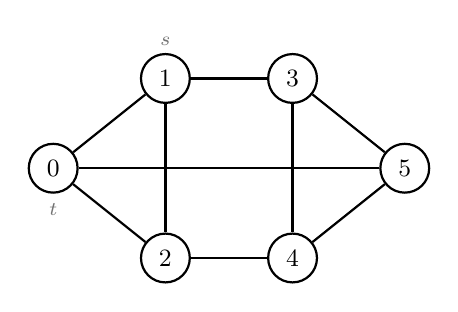
\begin{tikzpicture}[scale=0.95]
  \node[gv] (0) at (0,0) {0}; \node[gv] (1) at (1.5,1.2) {1}; \node[gv] (2) at (1.5,-1.2) {2};
  \node[gv] (3) at (3.2,1.2) {3}; \node[gv] (4) at (3.2,-1.2) {4}; \node[gv] (5) at (4.7,0) {5};
  \foreach \a/\b in {0/1,0/2,1/2,1/3,2/4,3/4,3/5,4/5,5/0} \draw[ge] (\a) -- (\b);
  \node[idx] at (0,-0.55) {$t$}; \node[idx] at (1.5,1.7) {$s$};
\end{tikzpicture}
\end{center}
DFS 的过程（栈从 \texttt{[0,1]} 开始）：
\begin{center}
\small
\begin{tabular}{lll}
\toprule
栈顶 & 看到的邻点 & 结果 \\
\midrule
$1$ & $0$（\texttt{dfn} $0$） & 已访问，$\texttt{low}[1]=0$，$\texttt{lowfrom}[1]=0$ \\
$1$ & $2$ & 新，$\texttt{dfn}[2]=2$，双亲 $1$，栈 \texttt{[0,1,2]} \\
$2$ & $0$ & 已访问，$\texttt{low}[2]=0$，$\texttt{lowfrom}[2]=0$ \\
$2$ & $1$ & 已访问（\texttt{dfn} $1\geqslant\texttt{low}[2]$，不更新） \\
$2$ & $4$ & 新，$\texttt{dfn}[4]=3$，双亲 $2$，栈 \texttt{[0,1,2,4]} \\
$4$ & $2$ & 已访问，$\texttt{low}[4]=2$，$\texttt{lowfrom}[4]=2$ \\
$4$ & $3$ & 新，$\texttt{dfn}[3]=4$，双亲 $4$，栈 \texttt{[0,1,2,4,3]} \\
$3$ & $1$ & 已访问，$\texttt{low}[3]=1$，$\texttt{lowfrom}[3]=1$ \\
$3$ & $4$ & 已访问，不更新 \\
$3$ & $5$ & 新，$\texttt{dfn}[5]=5$，双亲 $3$，栈 \texttt{[0,1,2,4,3,5]} \\
$5$ & $3$ & 已访问，$\texttt{low}[5]=4$，$\texttt{lowfrom}[5]=3$ \\
$5$ & $4$ & 已访问，$\texttt{low}[5]=3$，$\texttt{lowfrom}[5]=4$ \\
$5$ & $0$ & 已访问，$\texttt{low}[5]=0$，$\texttt{lowfrom}[5]=0$ \\
$5$ & （看完） & 出栈；$\texttt{low}[3]=0$，$\texttt{lowfrom}[3]=5$ \\
$3$ & （看完） & 出栈；$\texttt{low}[4]=0$，$\texttt{lowfrom}[4]=3$ \\
$4$ & $5$ & 已访问，不更新；然后看完，出栈（$\texttt{low}[2]=0$ 已经最小） \\
$2$ & （看完） & 出栈 \\
$1$ & $3$ & 已访问，不更新；看完，出栈 \\
$0$ & $1,2,5$ & 都已访问；出栈 \\
\bottomrule
\end{tabular}
\end{center}
结果：
\[
\begin{aligned}
&\texttt{dfn}=[0,1,2,4,3,5],&&\texttt{parent}=[-1,0,1,4,2,3],\\
&\texttt{low}=[0,0,0,0,0,0],&&\texttt{lowfrom}=[-1,0,0,5,3,0].
\end{aligned}
\]
DFS 树是路 $0-1-2-4-3-5$；返回边是 $02$、$13$、$45$、$50$。
\end{example}

\topic{三、st-编号算法}

算法维护一个栈，并把顶点分成\term{老点}（已经进过栈，\texttt{mark}$=1$）与\term{新点}。开始时只有 $s,t$ 是老点，栈为 \texttt{[t,s]}（$s$ 在顶上）。每一步：
\begin{enumerate}
\item 出栈一个顶点 $u$，给它下一个编号。
\item 对 $u$ 的每个是新点的孩子 $v$：从 $v$ 出发沿 \texttt{lowfrom} 往下走，把经过的新点依次标为老点，直到走到一个老点 $w$ 为止。得到路 $u,v,\dots,w$（中间都是刚标的老点）。把中间这些点进栈，使 $v$ 在最上面。
\item 对 $u$ 的每个是新点、并且 $\texttt{dfn}$ 比 $u$ 大的邻点 $v$（即从后代 $v$ 连到 $u$ 的返回边）：从 $v$ 出发沿 \texttt{parent} 往上走，同样标记、进栈，$v$ 在最上面。
\end{enumerate}

\begin{lstlisting}[language=Python]
def st_number(adj, s, t, dfn, parent, lowfrom):
    """2-连通图的 st-编号（讲义算法 2.10）。stn[v] 是 v 的编号 1..n。"""
    n = len(adj)
    stn = [-1] * n
    mark = [0] * n                 # 1 = 老点
    mark[s] = mark[t] = 1
    count = 1
    stack = [t, s]
    while stack:
        u = stack.pop()
        stn[u] = count             # 讲义此处误写为 stn[i]
        count += 1
        for v in adj[u]:           # 第 2 步：树边 u -> v
            if mark[v] == 0 and parent[v] == u:
                path, w = [], v
                while mark[w] == 0:
                    mark[w] = 1
                    path.append(w)
                    w = lowfrom[w]
                while path:
                    stack.append(path.pop())   # 最后一个先进栈，v 在最上面
        for v in adj[u]:           # 第 3 步：返回边 v -> u，v 是 u 的后代
            if mark[v] == 0 and dfn[v] > dfn[u]:
                path, w = [], v
                while mark[w] == 0:
                    mark[w] = 1
                    path.append(w)
                    w = parent[w]
                while path:
                    stack.append(path.pop())
    return stn

def st_numbering(adj, s, t):
    dfn, parent, low, lowfrom = dfn_low(adj, s, t)
    return st_number(adj, s, t, dfn, parent, lowfrom)
\end{lstlisting}

\begin{example}\label{ex:st-numbering:run}
接着\egref[上面的例子]{ex:st-numbering:dfs}。
\begin{center}
\small
\begin{tabular}{p{1.7cm}p{8.6cm}l}
\toprule
出栈，编号 & 第 2、3 步 & 之后的栈 \\
\midrule
$1$，编号 $1$ & 孩子 $2$ 是新点：标 $2$；$\texttt{lowfrom}[2]=0$ 是老点，停。路 $1,2,0$，$2$ 进栈。\newline
返回边：邻点 $3$ 新、$\texttt{dfn}[3]=4>1$：标 $3$；$\texttt{parent}[3]=4$ 新，标 $4$；$\texttt{parent}[4]=2$ 是老点，停。路 $1,3,4,2$，先进 $4$ 再进 $3$。 & \texttt{[0,2,4,3]} \\
$3$，编号 $2$ & 孩子 $5$ 新：标 $5$；$\texttt{lowfrom}[5]=0$ 老，停。路 $3,5,0$，$5$ 进栈。邻点 $1,4$ 都是老点。 & \texttt{[0,2,4,5]} \\
$5$，编号 $3$ & 邻点 $3,4,0$ 都是老点。 & \texttt{[0,2,4]} \\
$4$，编号 $4$ & 邻点都是老点。 & \texttt{[0,2]} \\
$2$，编号 $5$ & 邻点都是老点。 & \texttt{[0]} \\
$0$，编号 $6$ & & \texttt{[]} \\
\bottomrule
\end{tabular}
\end{center}
\texttt{stn=[6,1,5,2,4,3]}，即顺序 $1,3,5,4,2,0$。检查：$3$（编号 $2$）有邻点 $1$（$1$）与 $4$（$4$）；$5$（$3$）有 $3$（$2$）与 $0$（$6$）；$4$（$4$）有 $3$（$2$）与 $2$（$5$）；$2$（$5$）有 $1$（$1$）与 $0$（$6$）。每个中间顶点都有一小一大两个邻点。
\end{example}

\topic{四、为什么算法是对的}

\begin{theorem}\label{thm:st-numbering:correct}
（讲义定理 2.14）设 $G$ 是 $2$-连通图，$st\in E(G)$。则 \texttt{st\_numbering} 在 $O(n+m)$ 时间内给出 st-编号。特别地，每个 $2$-连通图对每条边 $st$ 都有 st-编号。
\end{theorem}

\begin{remark}[证明思路]
关键是两件事。第一，老点的集合始终“对祖先封闭”：一个点是老点，它的祖先都是老点。第二，每次进栈的一条路 $u_1u_2\dots u_k$（$u_1$ 刚出栈，$u_k$ 是原来的老点）中，$u_k$ 还在栈里，没有出栈；于是 $u_2,\dots,u_{k-1}$ 压在 $u_k$ 上面，编号依次落在 $u_1$ 与 $u_k$ 之间，并且依次递增。这样每个 $u_i$ 的两个路上邻点 $u_{i-1},u_{i+1}$ 一个编号小、一个编号大。
\end{remark}

\begin{proof}
\emph{(1) 老点集对祖先封闭。}开始时老点是 $t,s$，成立。第 2 步：$u$ 是老点，$v$ 是它的孩子。沿 \texttt{lowfrom} 走：若 $\texttt{lowfrom}[c]$ 是 $c$ 的孩子，就往下走一层；否则 $\texttt{lowfrom}[c]=w$ 是 $c$ 的一个邻点，$\texttt{dfn}[w]=\texttt{low}[c]=\texttt{low}[v]$（沿孩子走时 low 值不变）。由 (d)，$\texttt{low}[v]<\texttt{dfn}[u]$（$u\neq s$），或 $\texttt{low}[v]=0$（$u=s$），所以 $w$ 是 $u$ 的真祖先，由归纳假设是老点。路上从 $v$ 往下走过的点 $v=c_0,c_1,\dots,c_j$ 是一条树中往下的路；它们原来都是新点（若某个 $c_i$ 是老点，它的祖先 $v$ 也是老点，矛盾），所以路在 $c_j$ 之后才遇到老点 $w$。标完后，新的老点 $c_0,\dots,c_j$ 的祖先是 $u$ 的祖先（老点）与 $c_0,\dots,c_{i-1}$（刚标的），封闭性保持。第 3 步：从后代 $v$ 沿双亲往上走到第一个老点 $x$，把路上的点都标为老点；这些点的祖先是 $x$ 的祖先（老点）与路上的点，封闭性保持。

\emph{(2) 一个顶点出栈并处理完后，它的邻点全是老点。}$u$ 的邻点是它的双亲与祖先（由 (1) 是老点）、孩子（第 2 步之后都是老点）、以返回边相连的后代（第 3 步之后都是老点）。

\emph{(3) 每条进栈的路 $u_1,u_2,\dots,u_k$ 的终点 $u_k$ 不是 $u_1$，并且还在栈中。}第 2 步中 $u_k=w$ 是 $u$ 的真祖先，$\neq u_1$。第 3 步中，往上走时最晚在 $u$ 的孩子处遇到老点（第 2 步已经把 $u$ 的孩子都标成了老点），所以 $u_k\neq u_1$。$u_k$ 是老点，进过栈；若它已经出栈，由 (2) 它的邻点 $u_{k-1}$ 在那时已是老点，而 $u_{k-1}$ 直到这一步才被标记，矛盾。

\emph{(4) 编号。}进栈后，$u_2$ 在最上面，$u_{k-1}$ 在最下面，都在 $u_k$ 之上。栈是后进先出的，以后进栈的点都压在上面，所以 $u_2,u_3,\dots,u_{k-1},u_k$ 按这个顺序出栈，编号递增；$u_1$ 已经编号，比它们都小。于是对 $2\leqslant i\leqslant k-1$，$u_i$ 的邻点 $u_{i-1}$ 编号比它小，$u_{i+1}$ 编号比它大。

\emph{(5) 每个顶点恰好编号一次。}每个顶点至多被标记一次，标记时恰好进栈一次，出栈时编号。若最后还有新点，由 (1) 取一个双亲 $p$ 是老点的新点 $y$；$p$ 进过栈、出过栈，出栈时第 2 步会把孩子 $y$ 标为老点，矛盾。所以所有顶点都进栈、编号，编号是 $1,\dots,n$。$s$ 在栈顶，最先出栈，编号 $1$；$t$ 在栈底，最后出栈，编号 $n$。除 $s,t$ 外每个顶点都是作为某条路的中间点 $u_i$ 被标记的，由 (4) 它有一大一小两个邻点。

\emph{时间。}\texttt{dfn\_low} 是一次 DFS，$O(n+m)$。\texttt{st\_number} 中每个顶点出栈一次，出栈时扫描它的邻接表两遍；沿 \texttt{lowfrom} 或 \texttt{parent} 走的每一步都标记一个新点，总共 $n$ 步。合计 $O(n+m)$。
\end{proof}

讲义的证明给出了 (3)、(4) 的论证，但没有说明 (1) 为什么成立，也没有说明 (2)（“一旦点 $v$ 出栈后，$v$ 的邻点都会变成老点”）为什么成立，而这两点是 (3) 的依据。

\topic{五、low 值的另一个用处：割点}

st-编号要求 $2$-连通。反过来，low 值可以用来找出一个连通图的全部割点，从而判断它是否 $2$-连通。这里用只算返回边的 low 值（不算通往双亲的树边）。

\begin{proposition}\label{prop:st-numbering:cut}
在连通图的 DFS 树（根为 $r$）中：$r$ 是割点当且仅当它有至少两个孩子；$u\neq r$ 是割点当且仅当它有一个孩子 $c$，使 $T_c$ 中没有返回边连到 $u$ 的真祖先，即 $\texttt{low}'[c]\geqslant\texttt{dfn}[u]$，其中 $\texttt{low}'[c]=\min(\{\texttt{dfn}[c]\}\cup\{\texttt{dfn}[w]: T_c$ 中某点与 $w$ 由返回边相连$\})$。
\end{proposition}
\begin{proof}
由 (c)，不同孩子的子树之间没有边，$T_c$ 只通过树边 $cu$ 与返回边连到外面，返回边只连到祖先。$u\neq r$：若某个孩子 $c$ 的 $T_c$ 没有返回边连到 $u$ 的真祖先，删去 $u$ 后 $T_c$ 与 $r$ 不连通；反之，若每个孩子的子树都有返回边连到真祖先，删去 $u$ 后每个 $T_c$ 都连到 $r$ 所在的部分（含 $u$ 的全部真祖先，它们由树边相连），$G-u$ 连通。$r$：孩子的子树之间没有边，有两个孩子时删去 $r$ 不连通；只有一个孩子时 $T-r$ 仍是一棵树。
\end{proof}

\begin{lstlisting}[language=Python]
def cut_vertices(adj, r=0):
    """连通图的全部割点（从 r 出发的一次 DFS）。"""
    n = len(adj)
    dfn, parent, low = [-1] * n, [-1] * n, [0] * n
    children = [0] * n
    cur = [0] * n
    dfn[r] = low[r] = 0
    num, stack, cut = 0, [r], set()
    while stack:
        u = stack[-1]
        if cur[u] < len(adj[u]):
            v = adj[u][cur[u]]
            cur[u] += 1
            if dfn[v] == -1:
                num += 1
                dfn[v] = low[v] = num
                parent[v] = u
                children[u] += 1
                stack.append(v)
            elif v != parent[u]:                 # 返回边（不算通往双亲的树边）
                low[u] = min(low[u], dfn[v])
        else:
            stack.pop()
            p = parent[u]
            if p != -1:
                low[p] = min(low[p], low[u])
                if p != r and low[u] >= dfn[p]:
                    cut.add(p)
    if children[r] >= 2:
        cut.add(r)
    return cut
\end{lstlisting}

（这个程序假定图是简单图：若有重边，“$v\neq$ 双亲”会把与双亲之间的第二条边也排除掉。）

\topic{小结}

\begin{itemize}
\item DFS 树的返回边只连接祖先与后代，$2$-连通性等价于每棵子树都有返回边越过双亲（性质 (d)）。
\item low 值记录子树“最高能连到哪里”，\texttt{lowfrom} 记录这条连接怎么走。
\item st-编号算法每次从刚编号的点出发，沿 \texttt{lowfrom}（往下再跳上去）或 \texttt{parent}（往上）找一条通向老点的路，把路上的点压在那个老点上面。正确性靠两件事：老点集对祖先封闭；路的终点还在栈中。
\end{itemize}

\homework{st-编号的练习}[st-编号]

\exercisepart{练习}

\begin{exercises}{A}{DFS 树与 st-编号}
\item\label{ex:st-numbering:A1} 证明定理~\ref{thm:st-numbering:correct} 的逆命题：设 $n\geqslant3$，$st\in E(G)$。若 $G$ 有 st-编号，则 $G$ 是 $2$-连通的。
\begin{solution}
由定理~\ref{thm:st-numbering:prefix}，$G$ 连通（取 $i=n-1$，前缀与 $\{t\}$ 都连通，$t$ 有编号更小的邻点）。设 $x$ 是割点，$G-x$ 的一个分支 $B$。

若 $s,t\notin B$：取 $B$ 中编号最大的顶点 $b$，它有一个编号更大的邻点，不在 $B$ 中，只能是 $x$；取 $B$ 中编号最小的顶点 $b'$，它有编号更小的邻点，只能是 $x$。于是 $\text{编号}(x)>\text{编号}(b)\geqslant\text{编号}(b')>\text{编号}(x)$，矛盾。

若 $s$ 或 $t$ 在 $B$ 中：$st$ 是边，$x\notin\{s,t\}$ 时 $s,t$ 在 $G-x$ 的同一个分支中；取另一个不含 $s,t$ 的分支，回到上一种情形。$x=s$ 时，取 $G-s$ 中不含 $t$ 的分支 $B$，其中编号最小的顶点要有编号更小的邻点，只能是 $s$；编号最大的顶点要有编号更大的邻点，只能是 $s$，而 $s$ 的编号是 $1$，矛盾。$x=t$ 对称。
\end{solution}

\item\label{ex:st-numbering:A2} 在\egref[例子]{ex:st-numbering:dfs}的图上取 $s=0$，$t=1$，写出 \texttt{dfn}、\texttt{low}、\texttt{lowfrom} 与 st-编号。
\begin{solution}
从 $t=1$ 进入 $s=0$：栈 \texttt{[1,0]}。$0$ 看 $1$（老，\texttt{low[0]=0}，\texttt{lowfrom[0]=1}）、$2$（新，\texttt{dfn}$=2$）；$2$ 看 $0$（\texttt{dfn} $1$，\texttt{low[2]=1}）、$1$（\texttt{dfn} $0$，\texttt{low[2]=0}，\texttt{lowfrom[2]=1}）、$4$（新，$3$）；$4$ 看 $2$（\texttt{low[4]=2}）、$3$（新，$4$）；$3$ 看 $1$（\texttt{low[3]=0}，\texttt{lowfrom[3]=1}）、$4$、$5$（新，$5$）；$5$ 看 $3$（\texttt{low[5]=4}）、$4$（$3$）、$0$（$1$，\texttt{lowfrom[5]=0}）；$5$ 出栈，\texttt{low[3]} 已是 $0$；$3$ 出栈，\texttt{low[4]=0}，\texttt{lowfrom[4]=3}；$4$、$2$、$0$、$1$ 依次出栈。
\[
\begin{aligned}
&\texttt{dfn}=[1,0,2,4,3,5],&&\texttt{parent}=[1,-1,0,4,2,3],\\
&\texttt{low}=[0,0,0,0,0,1],&&\texttt{lowfrom}=[1,-1,1,1,3,0].
\end{aligned}
\]
st-编号：出栈 $0$（编号 $1$）；孩子 $2$ 新，标 $2$，$\texttt{lowfrom}[2]=1$ 老，进栈 $2$；返回边 $5$（$\texttt{dfn}\,5>1$），标 $5$，$\texttt{parent}[5]=3$ 新，标 $3$，$\texttt{parent}[3]=4$ 新，标 $4$，$\texttt{parent}[4]=2$ 老；进栈 $4,3,5$，栈 \texttt{[1,2,4,3,5]}。出栈 $5$（$2$）、$3$（$3$）、$4$（$4$）、$2$（$5$）、$1$（$6$），途中没有新点。\texttt{stn=[1,6,5,3,4,2]}，顺序 $0,5,3,4,2,1$。检查：$5$ 的邻点 $0$（$1$）、$3$（$3$）；$3$ 的邻点 $5$（$2$）、$4$（$4$）；$4$ 的邻点 $3$（$3$）、$2$（$5$）；$2$ 的邻点 $0$（$1$）、$1$（$6$）。
\end{solution}

\item\label{ex:st-numbering:A3} 用 \texttt{cut\_vertices} 找出图 \texttt{[(0,1),(1,2),(2,0),(2,3),(3,4),(4,5),(5,3)]}（两个三角形由一条边 $23$ 相连）的割点，写出 DFS 过程中的 \texttt{dfn} 与 \texttt{low}。
\begin{solution}
邻接表 \texttt{[[1,2],[0,2],[1,0,3],[2,4,5],[3,5],[4,3]]}，从 $0$ 出发：$0\to1\to2$（\texttt{dfn} $0,1,2$）；$2$ 看 $1$（双亲，跳过）、$0$（返回边，\texttt{low[2]=0}）、$3$（新，$3$）；$3\to4$（$4$）$\to5$（$5$）；$5$ 看 $4$（双亲）、$3$（返回边，\texttt{low[5]=3}）。出栈 $5$：\texttt{low[4]=min(4,3)=3}；$p=4\neq0$，$\texttt{low}[5]=3<\texttt{dfn}[4]=4$，$4$ 不是割点。出栈 $4$：\texttt{low[3]=3}；$\texttt{low}[4]=3\geqslant\texttt{dfn}[3]=3$，$3$ 是割点。出栈 $3$：$\texttt{low}[2]=0$；$\texttt{low}[3]=3\geqslant\texttt{dfn}[2]=2$，$2$ 是割点。出栈 $2$：\texttt{low[1]=0}；$0<1$，$1$ 不是割点。出栈 $1$：$p=0$ 是根，不判断。根 $0$ 只有一个孩子。割点为 $\{2,3\}$。最终 $\texttt{dfn}=[0,1,2,3,4,5]$，$\texttt{low}=[0,0,0,3,3,3]$。
\end{solution}
\end{exercises}

\end{document}
